\label{section:c}
In this chapter, we will discuss the experimental techniques that are used to fabricate twisted bilayer graphene devices. The device structure is as shown in fig. \ref{fig:stack}: (1) Top gate is Cr/Au deposition with 5 nm Chromium and 50 nm gold, (2) top hBN is thick hBN around 30 nm, (3) two monolayer graphenes twisted at an angle, (4) tunnel hBN is thin hBN around 2nm, (5) Gold pad with multiple lines is Cr/Au deposition with 5 nm Chromium and 10 nm gold, and (6) $Si-SiO_2$ is Si with an oxide layer on top, around 285 nm. The fabrication of the devices is a very important step as it determines whether we will observe certain features in our measurements. In this experiment, we wish to have a twist angle between the graphene to be close to magic angle, i.e., $1.1 ^o$. The thickness of tunnel hBN and the alignment of the flakes are also important in the making of these devices.

\begin{figure}[H]
	\centering
	\includegraphics[width=\linewidth]{figures/stack.jpg}
	\caption{The device structure that is required in twisted bilayer graphene tunneling experiment.}
	\label{fig:stack}
\end{figure}

\section{Exfoliation of graphene and hBN}

There are various ways of preparing graphene flakes. \cite{Bhuyan2016, Yi2015} The notable ones are Mechanical Exfoliation and Chemical Vapour Deposition (CVD). CVD can be used to grow large scale continuous graphene sheets in the order of centimetres. But this method doesn't produce graphene flakes that have good electron mobility like mechanical exfoliation. We use Mechanical Exfoliation in our experiments.

In this method, we exfoliate graphene flakes onto $Si-SiO_2$ substrate. We have $Si-SiO_2$ substrate cut into small pieces of approximately 1.5cm $\times$ 1.5cm. We then clean the wafers using sonication, in which the wafers are put in a beaker of acetone and sonicated in either normal or soft mode for 5mins. The wafers are then dipped in IPA and blow dried using $N_2$. These steps remove the organic adsorbates from the substrate surface. We worked with three variations of Mechanical Exfoliation:

\begin{itemize}
	\item Conventional Exfoliation:
	We place a chunk of natural graphite on a Scotch tape and subsequently cleave it to the fresh regions of the tape, uniformly distributing on the tape. This tape is called the Master Tape. The graphite crystals are then transferred from Master Tape onto a new tape by adhering the second tape to the first and slowly peeling it away. This process is repeated till thin translucent graphite crystals containing tape is made. This step ensures that we have flat regions of graphite on the tape surface. This tape is then stuck on the substrate, and we gently apply pressure using a plastic dropper. We peel off the tape slowly. When the tape is removed, van der Waals force between the substrate and the top layers of the graphite crystals will pull down flakes of graphite ranging from 0.34nm (monolayer graphene) to hundreds of nanometers. Fig. \ref{fig:exfo} shows the conventional exfoliation process.
	
	\begin{figure}[H]
		\centering
		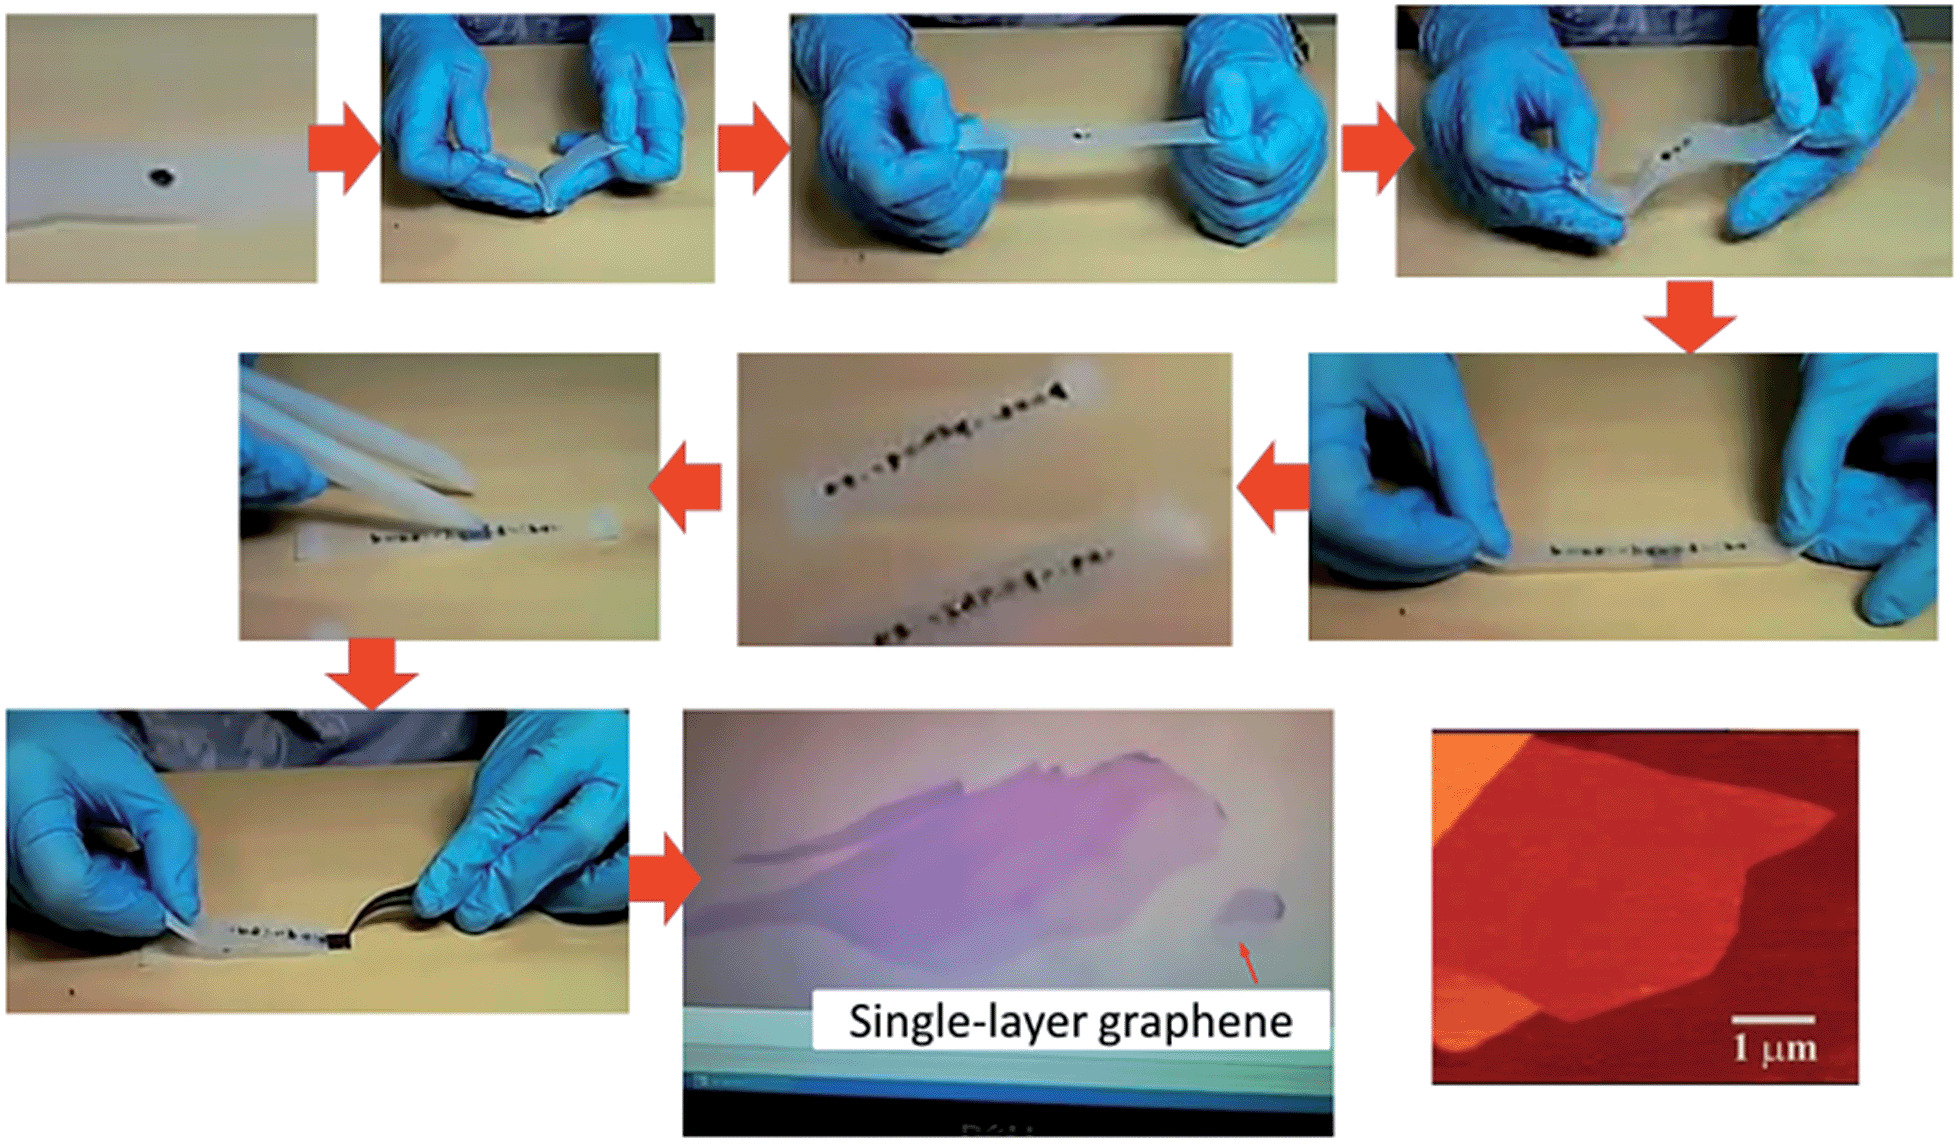
\includegraphics[width=\linewidth]{figures/exfo.jpg}
		\caption{Conventional exfoliation process. Figure adapted from \cite{Yi2015}}
		\label{fig:exfo}
	\end{figure}
	
	\item Hot Exfoliation:
	We follow the same steps as in conventional exfoliation, with one variation. We heat the substrate using a hot plate at $100 ^o C$ for 2-3 mins before sticking the tape onto it. This will improve the adhesion between graphite crystals and the substrate. Fig. \ref{fig:hot} shows the heater used at lab
	
	\begin{figure}[H]
		\centering
		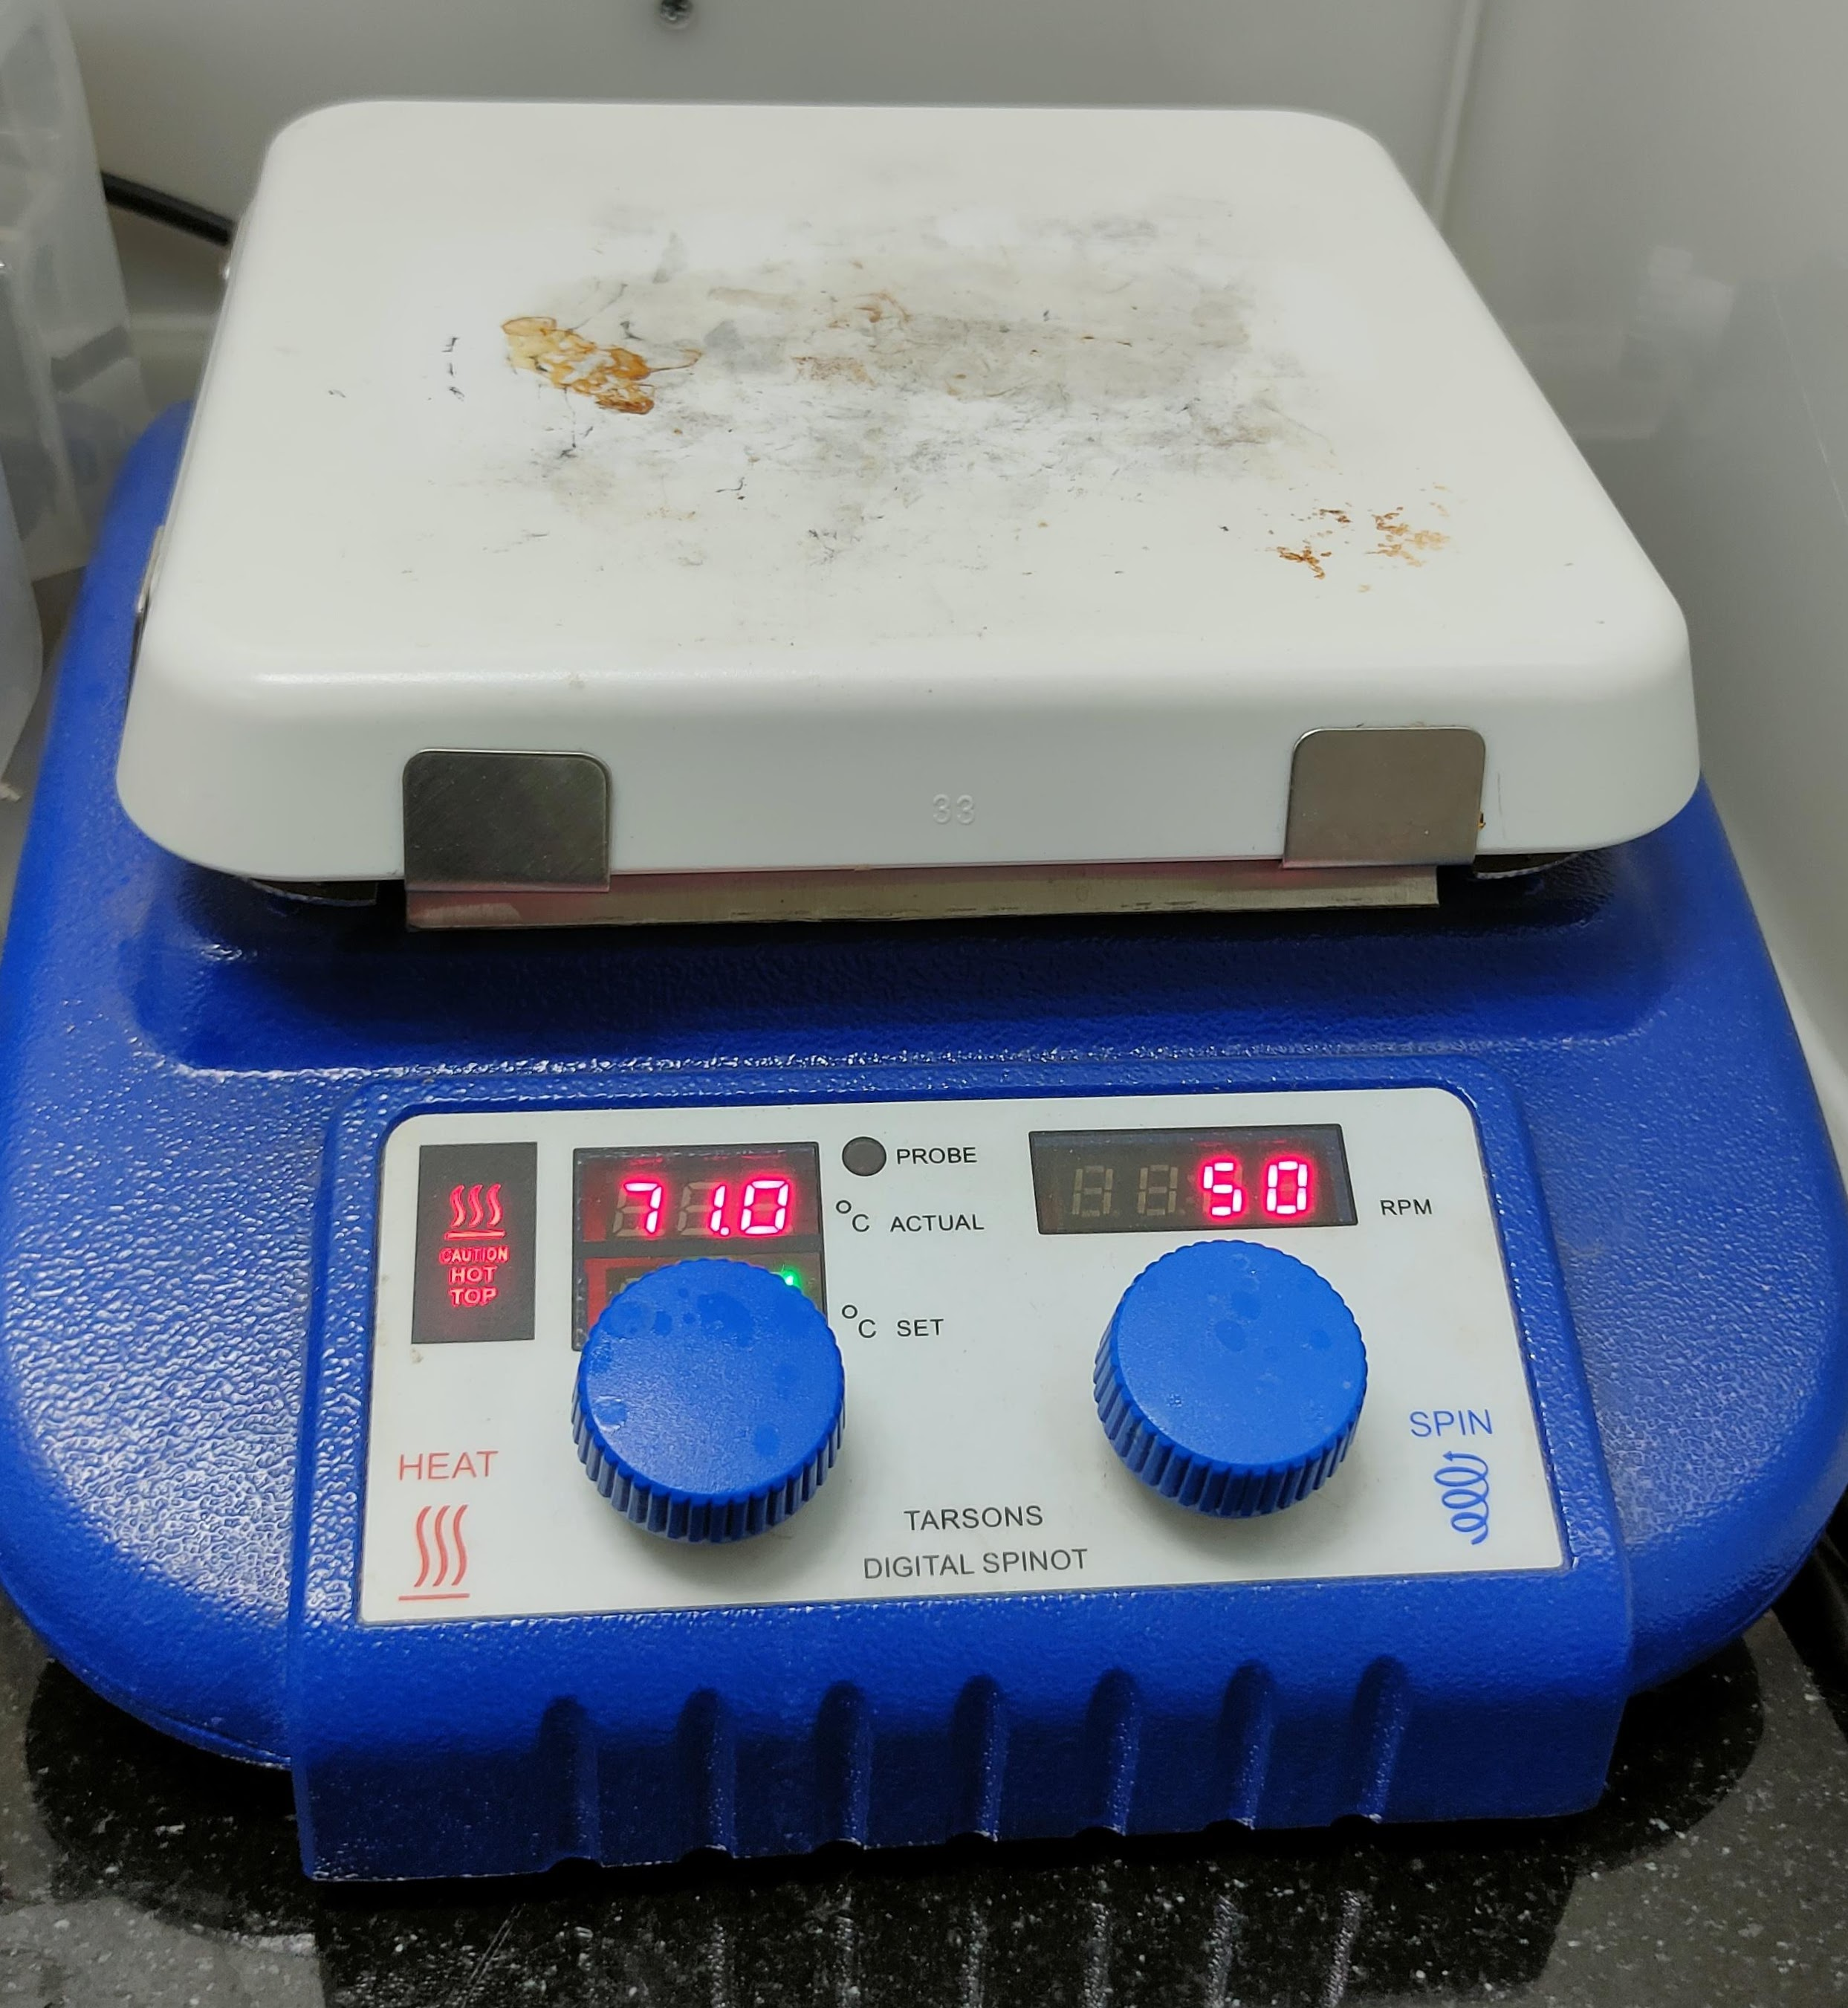
\includegraphics[width=0.4\linewidth]{figures/heat.jpg}
		\caption{Heater at lab that has a hot plate used during exfoliation.}
		\label{fig:hot}
	\end{figure}
	
	\item Oxygen Plasma Exfoliation:
	Here also we follow the same steps as in conventional exfoliation, with one variation. We clean the substrate using oxygen plasma cleaner before sticking the tape on it. The plasma cleaner setup at the lab consists of: (1) High power expanded plasma cleaner from Harrick Plasma (Model: PDC-002-HP, RF frequency: MHz range, Input power: 200W, Power applied to RF coil: 45 W), (2) Vacuum gauge, (3) Dry vacuum pump, and (4) Oxygen cylinder (see fig. \ref{fig:plcl}). This step helps remove adsorbates from the substrate's surface, hence improving the flake transfer, both in number and size, by increasing the adhesion of flakes to the substrate.
\end{itemize}

\begin{figure}[H]
	\centering
	\begin{subfigure}[t]{0.7\textwidth}
		\centering
		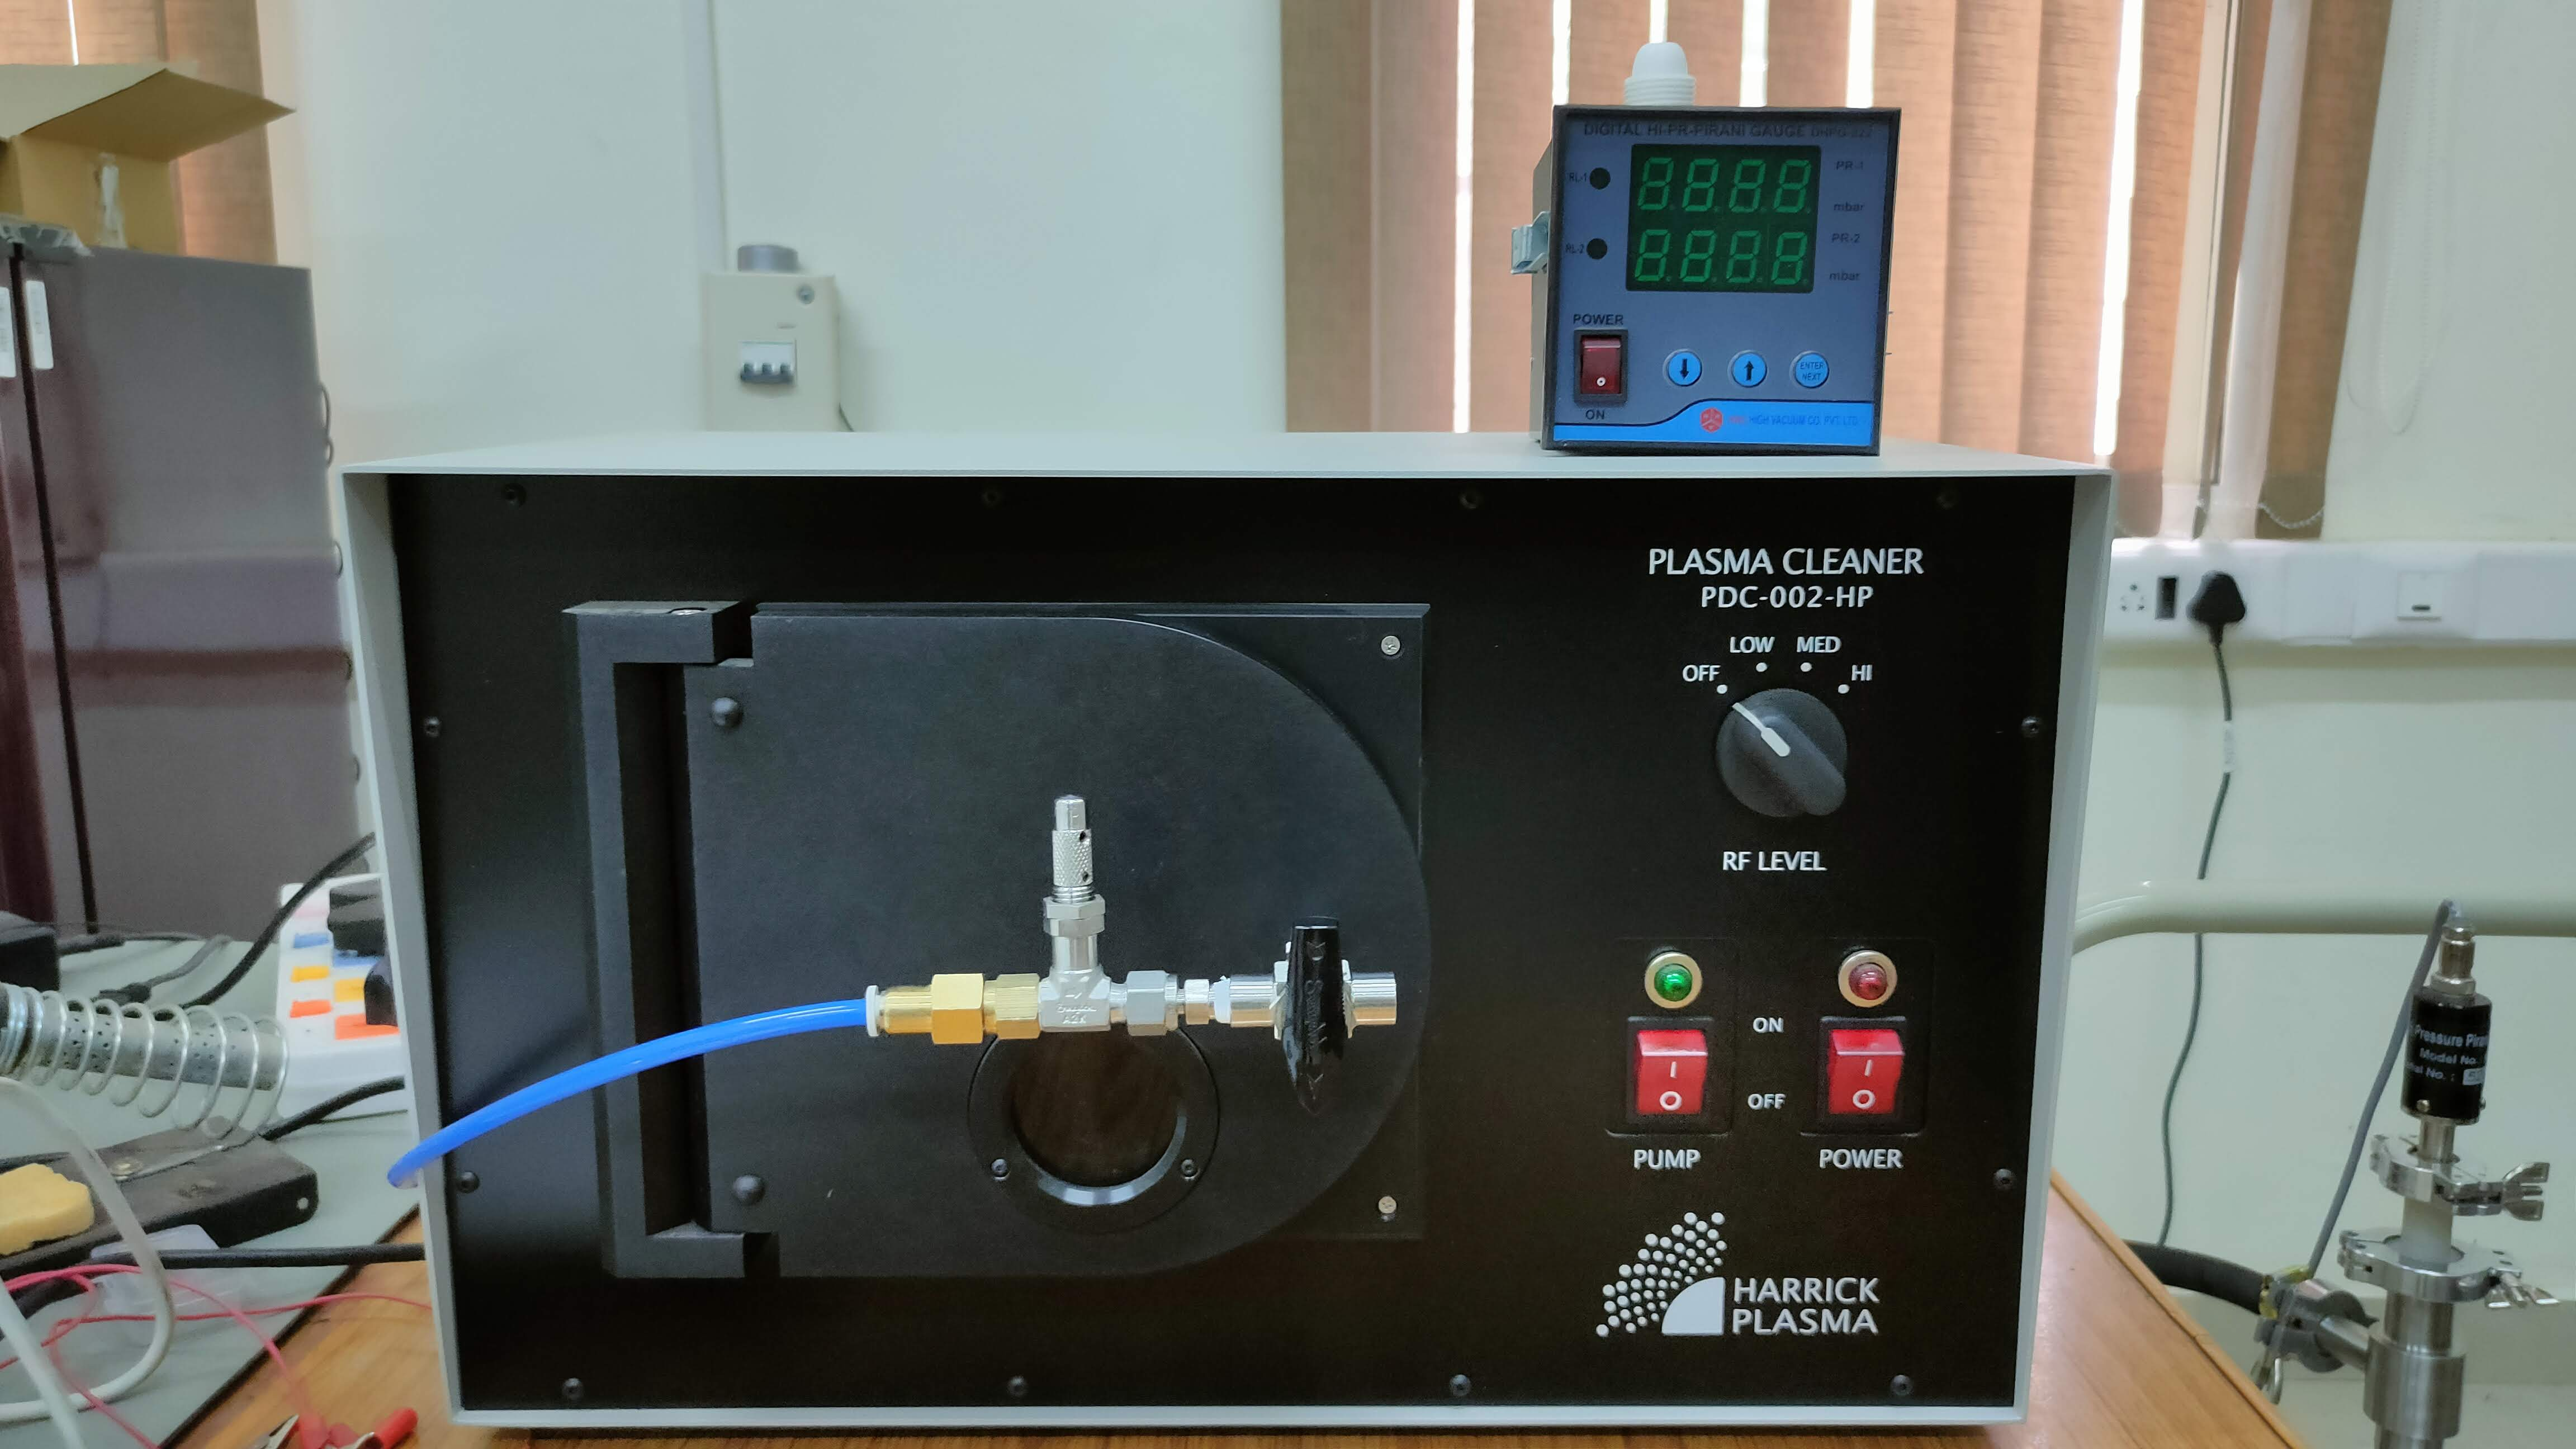
\includegraphics[width=\textwidth]{figures/plcl.jpg}
		\caption{Plasma cleaner and vacuum gauge}
	\end{subfigure}
	
	\begin{minipage}{.45\linewidth}
		\begin{subfigure}[b]{0.7\textwidth}
			\centering
			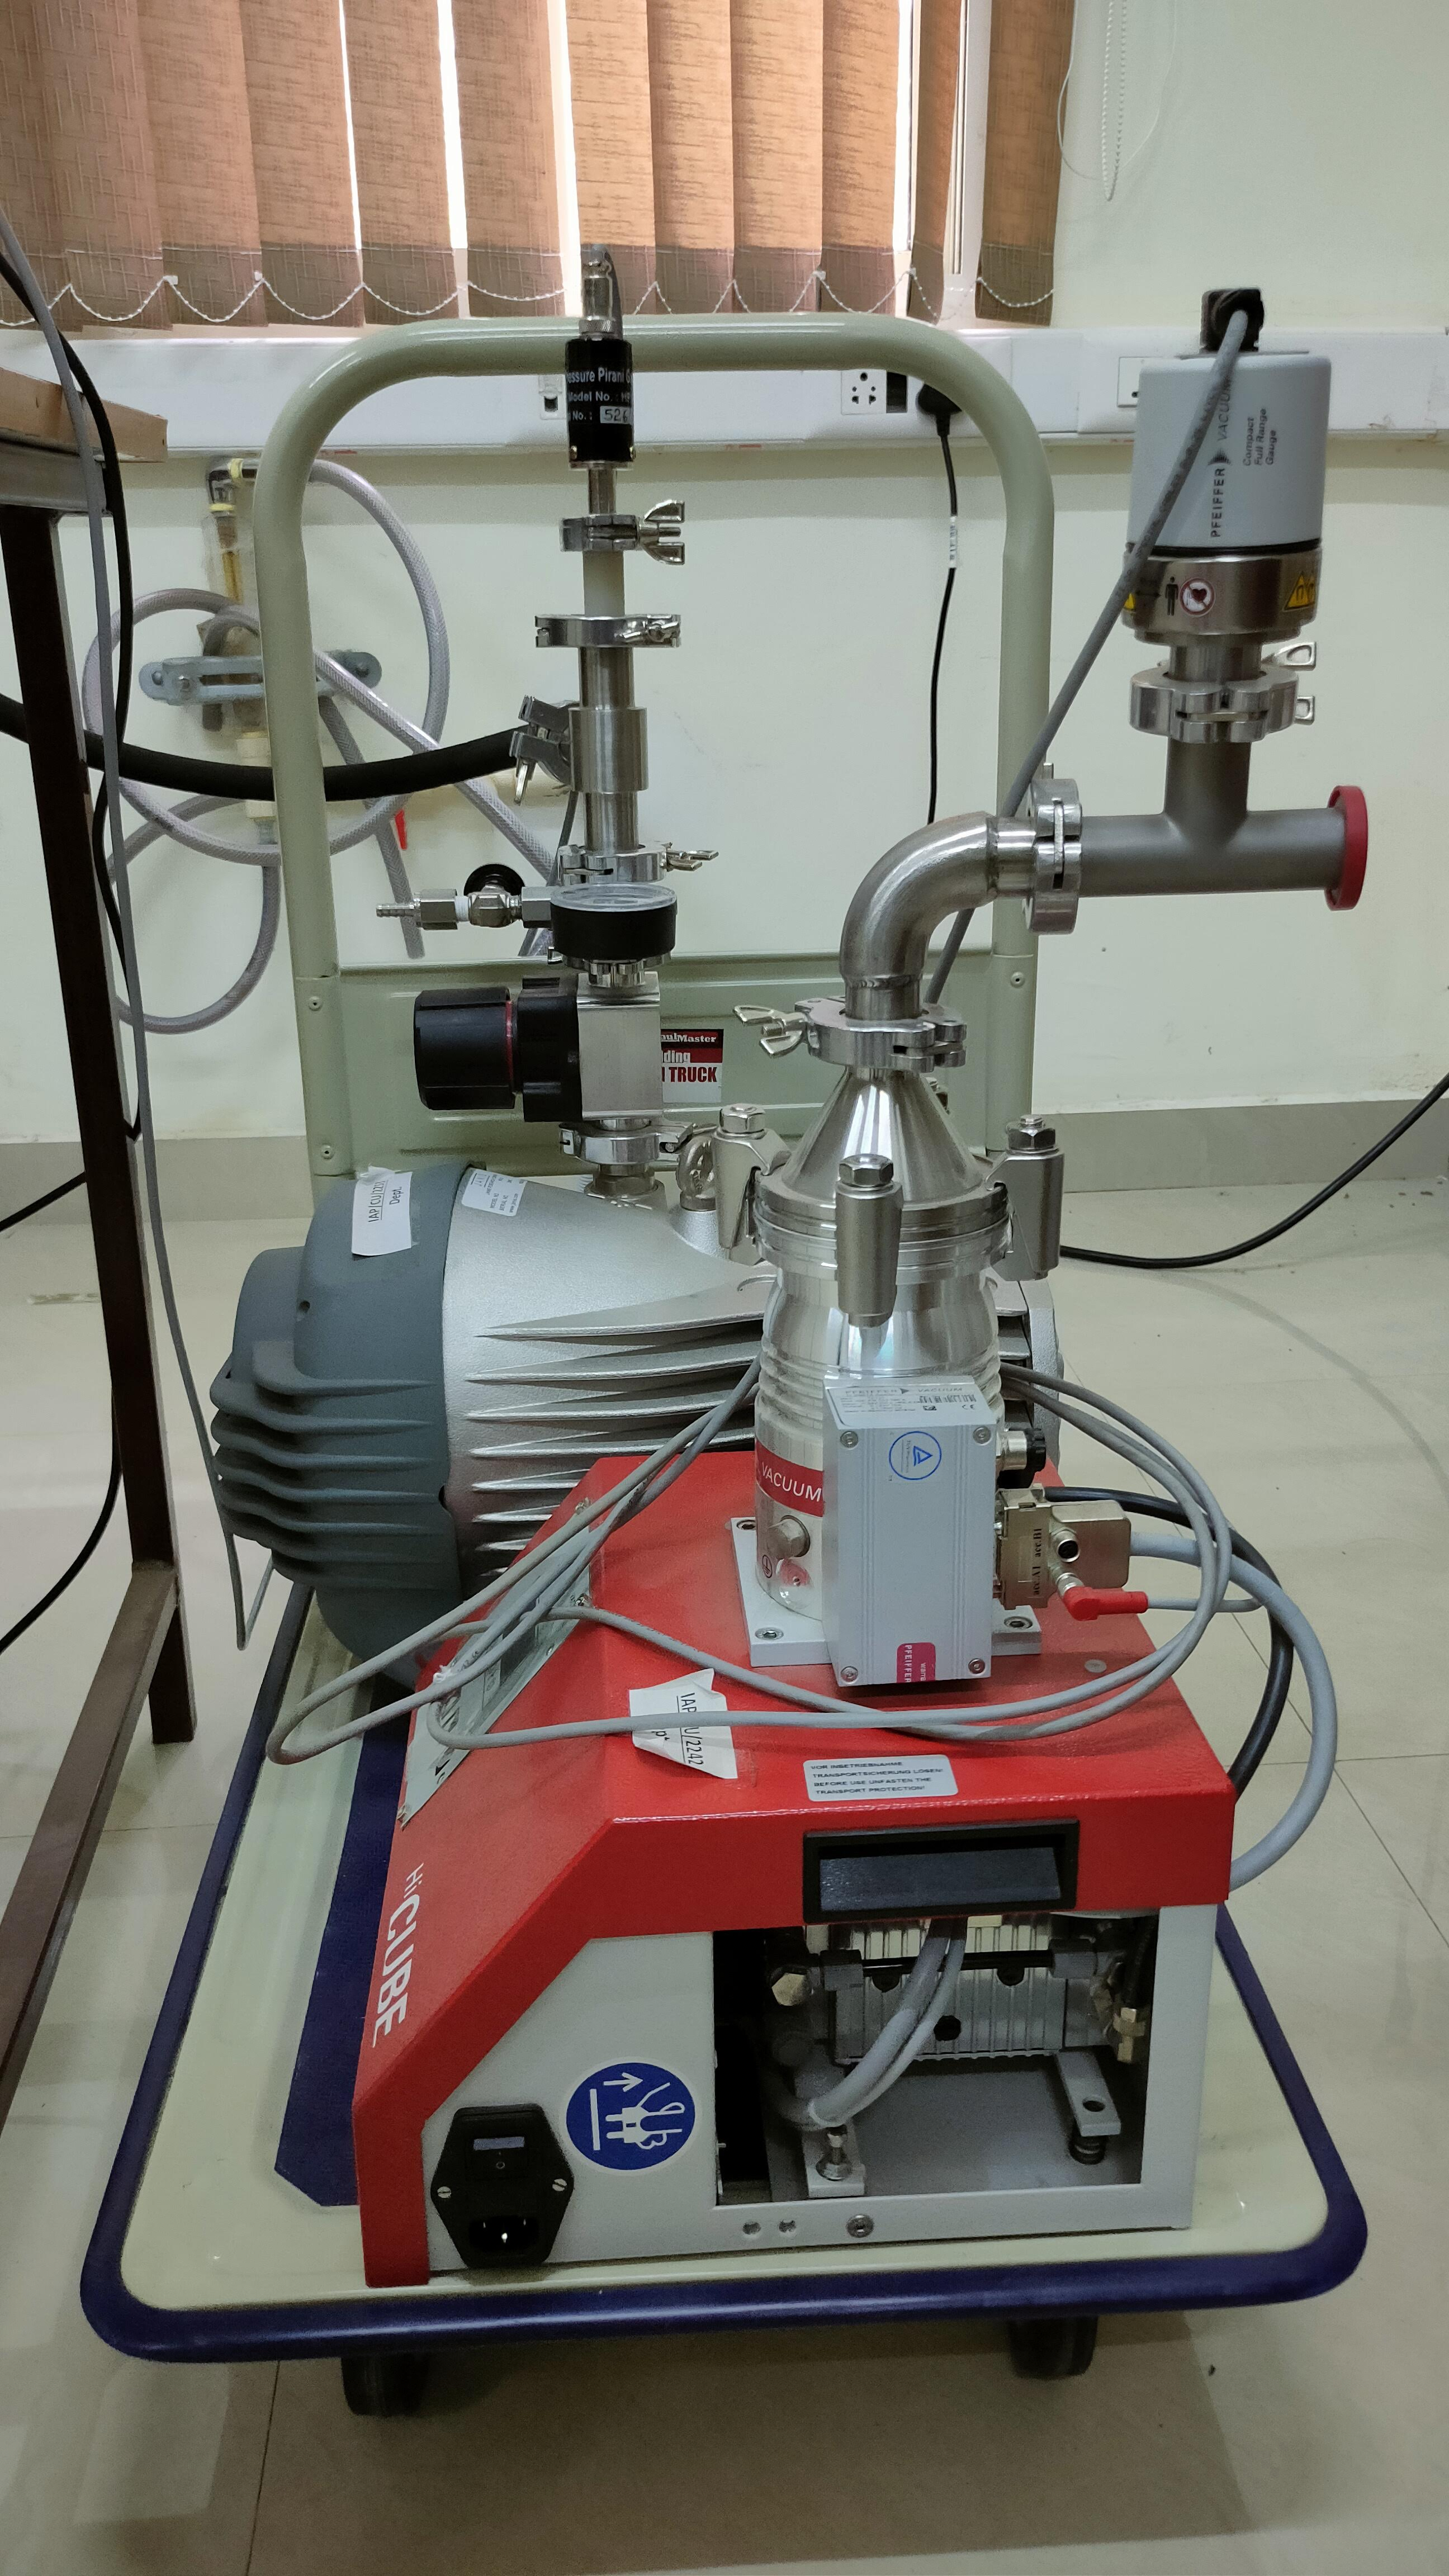
\includegraphics[width=\textwidth]{figures/plcl2.jpg}
			\caption{Dry vacuum pump}
		\end{subfigure}
	\end{minipage}%
	\begin{subfigure}{0.45\textwidth}
		\centering
		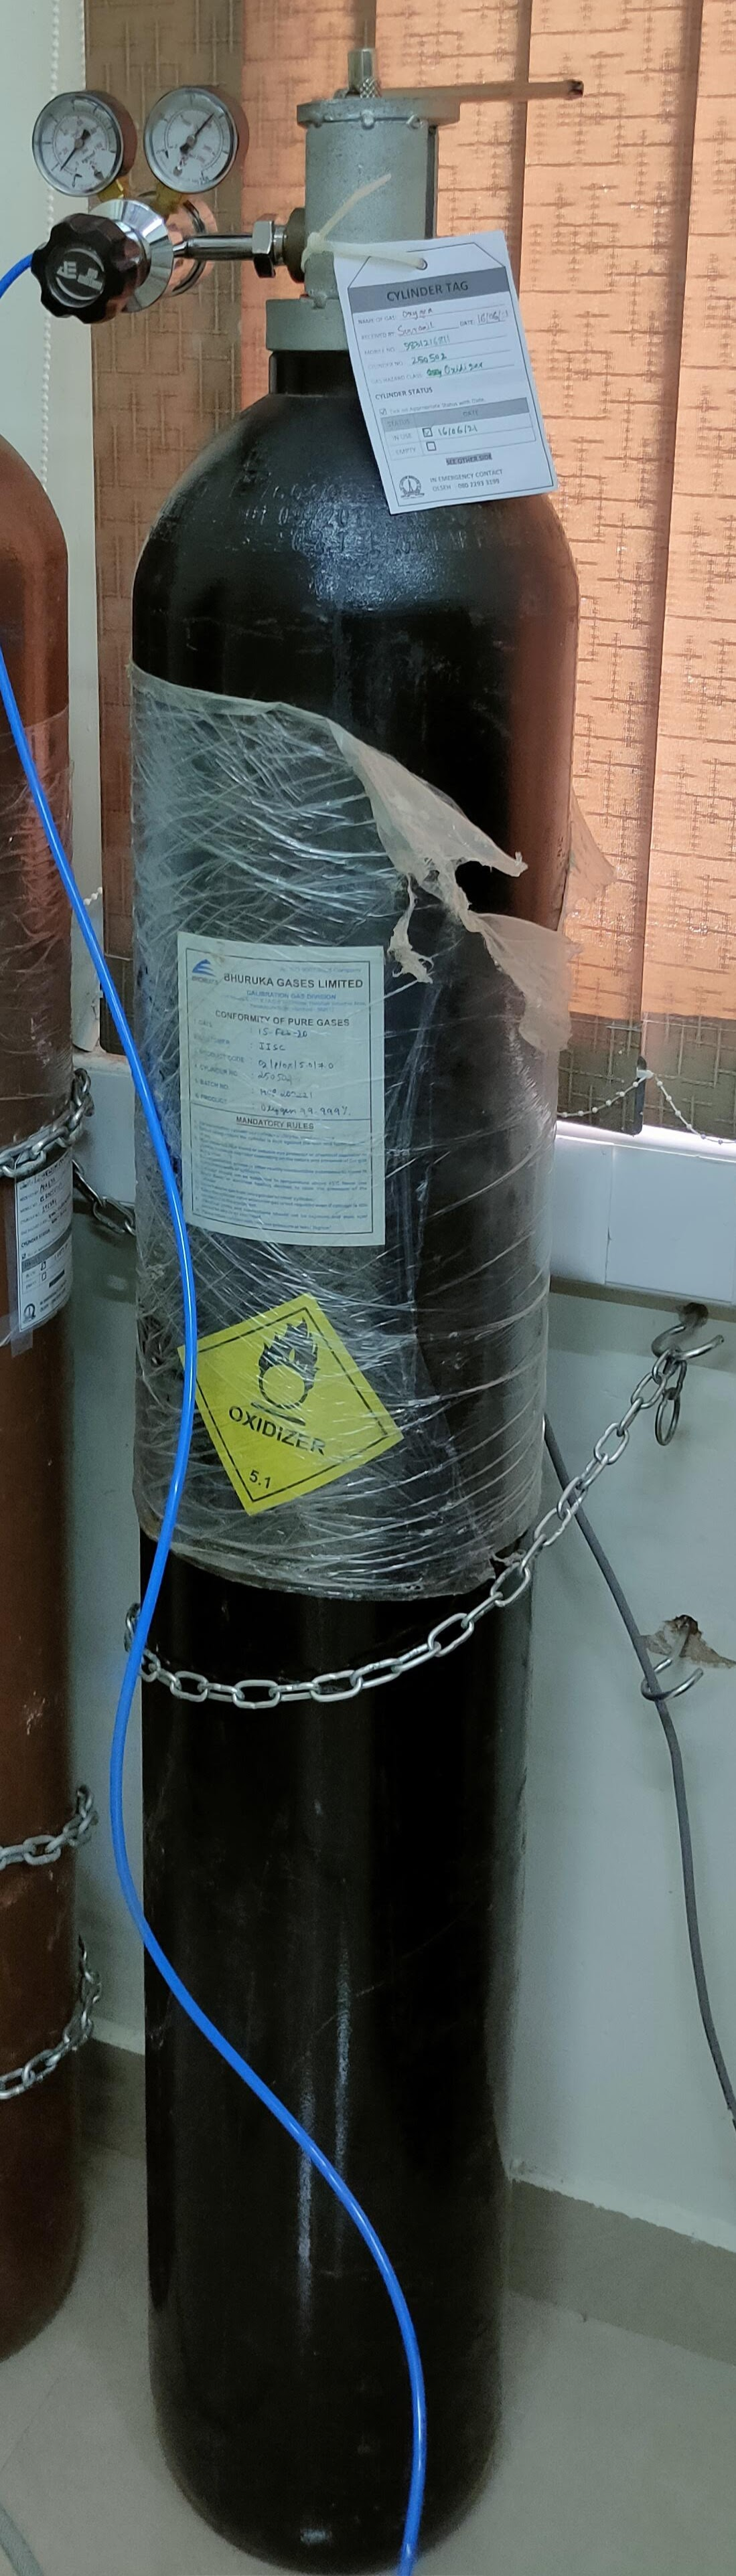
\includegraphics[width=0.35\textwidth]{figures/plcl3.jpg}
		\caption{Oxygen cylinder}
	\end{subfigure}
	\caption{Plasma cleaner setup at lab.}
	\label{fig:plcl}
\end{figure}

We use Hot Exfoliation to get graphene flakes for our devices. The reason we don't use oxygen plasma is that the flakes obtained by this method are hard to pickup using the dry transfer method (section \ref{section:f}). We are looking for large monolayer graphene.

We use conventional Mechanical Exfoliation to get hexagonal Boron Nitride (hBN) flakes. The method is similar to that for graphene, with hBN crystals used instead of graphite while making the master tape. We use hBN crystals from Watanabe, K. and Taniguchi, T., NIMS, Japan, known to give good quality thin flakes. \cite{hbn} We are looking for hBN with two different thicknesses - less than or close to 2 nm (thin hBN) \cite{Chandni} and around 30nm (thick hBN). The thin hBN is used as the tunneling barrier between twBLG and gold pads, while the thick hBN is used as top and bottom hBN next to the gate.

After exfoliation, the substrates with flakes are stored in boxes (fig. \ref{fig:box}) and kept in desicators (fig. \ref{fig:des}), which are later subject to flake selection.

\begin{figure}[H]
	\centering
	\begin{subfigure}{.5\linewidth}
		\centering
		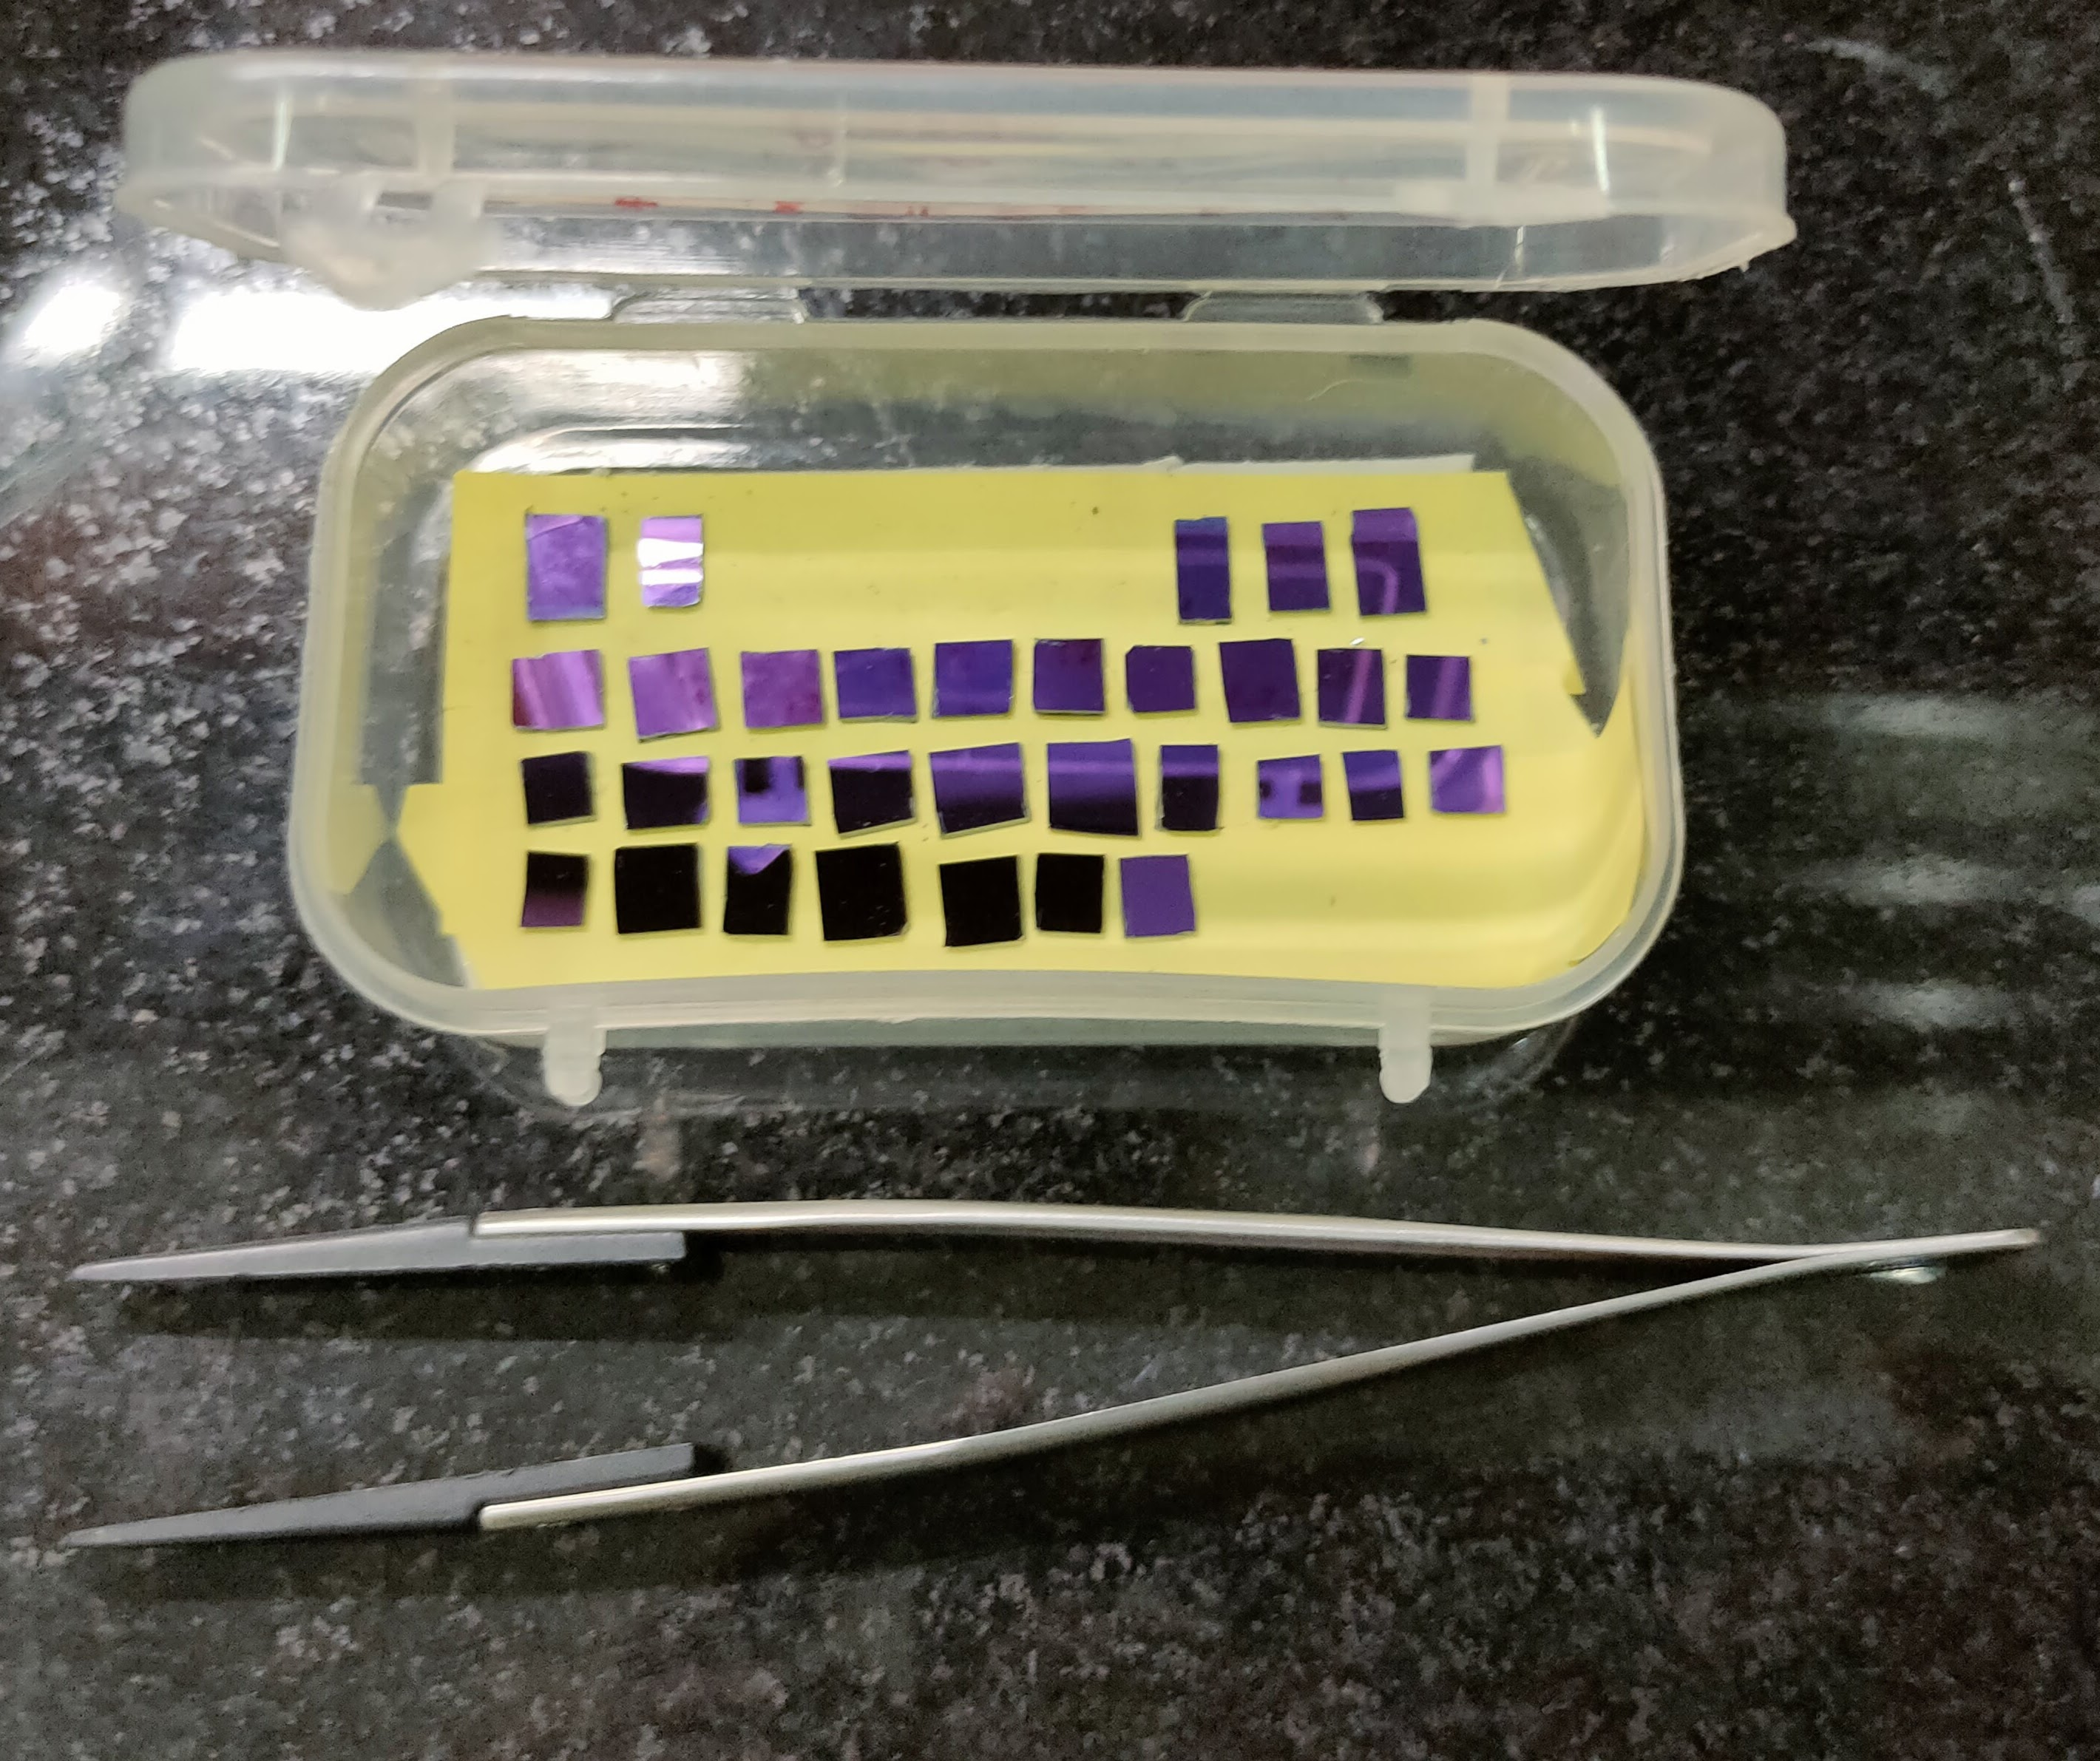
\includegraphics[width=.8\linewidth]{figures/box}
		\caption{A box containing $Si-SiO_2$ substrates \\ with graphene and hBN flakes on them.}
		\label{fig:box}
	\end{subfigure}%
	\begin{subfigure}{.5\linewidth}
		\centering
		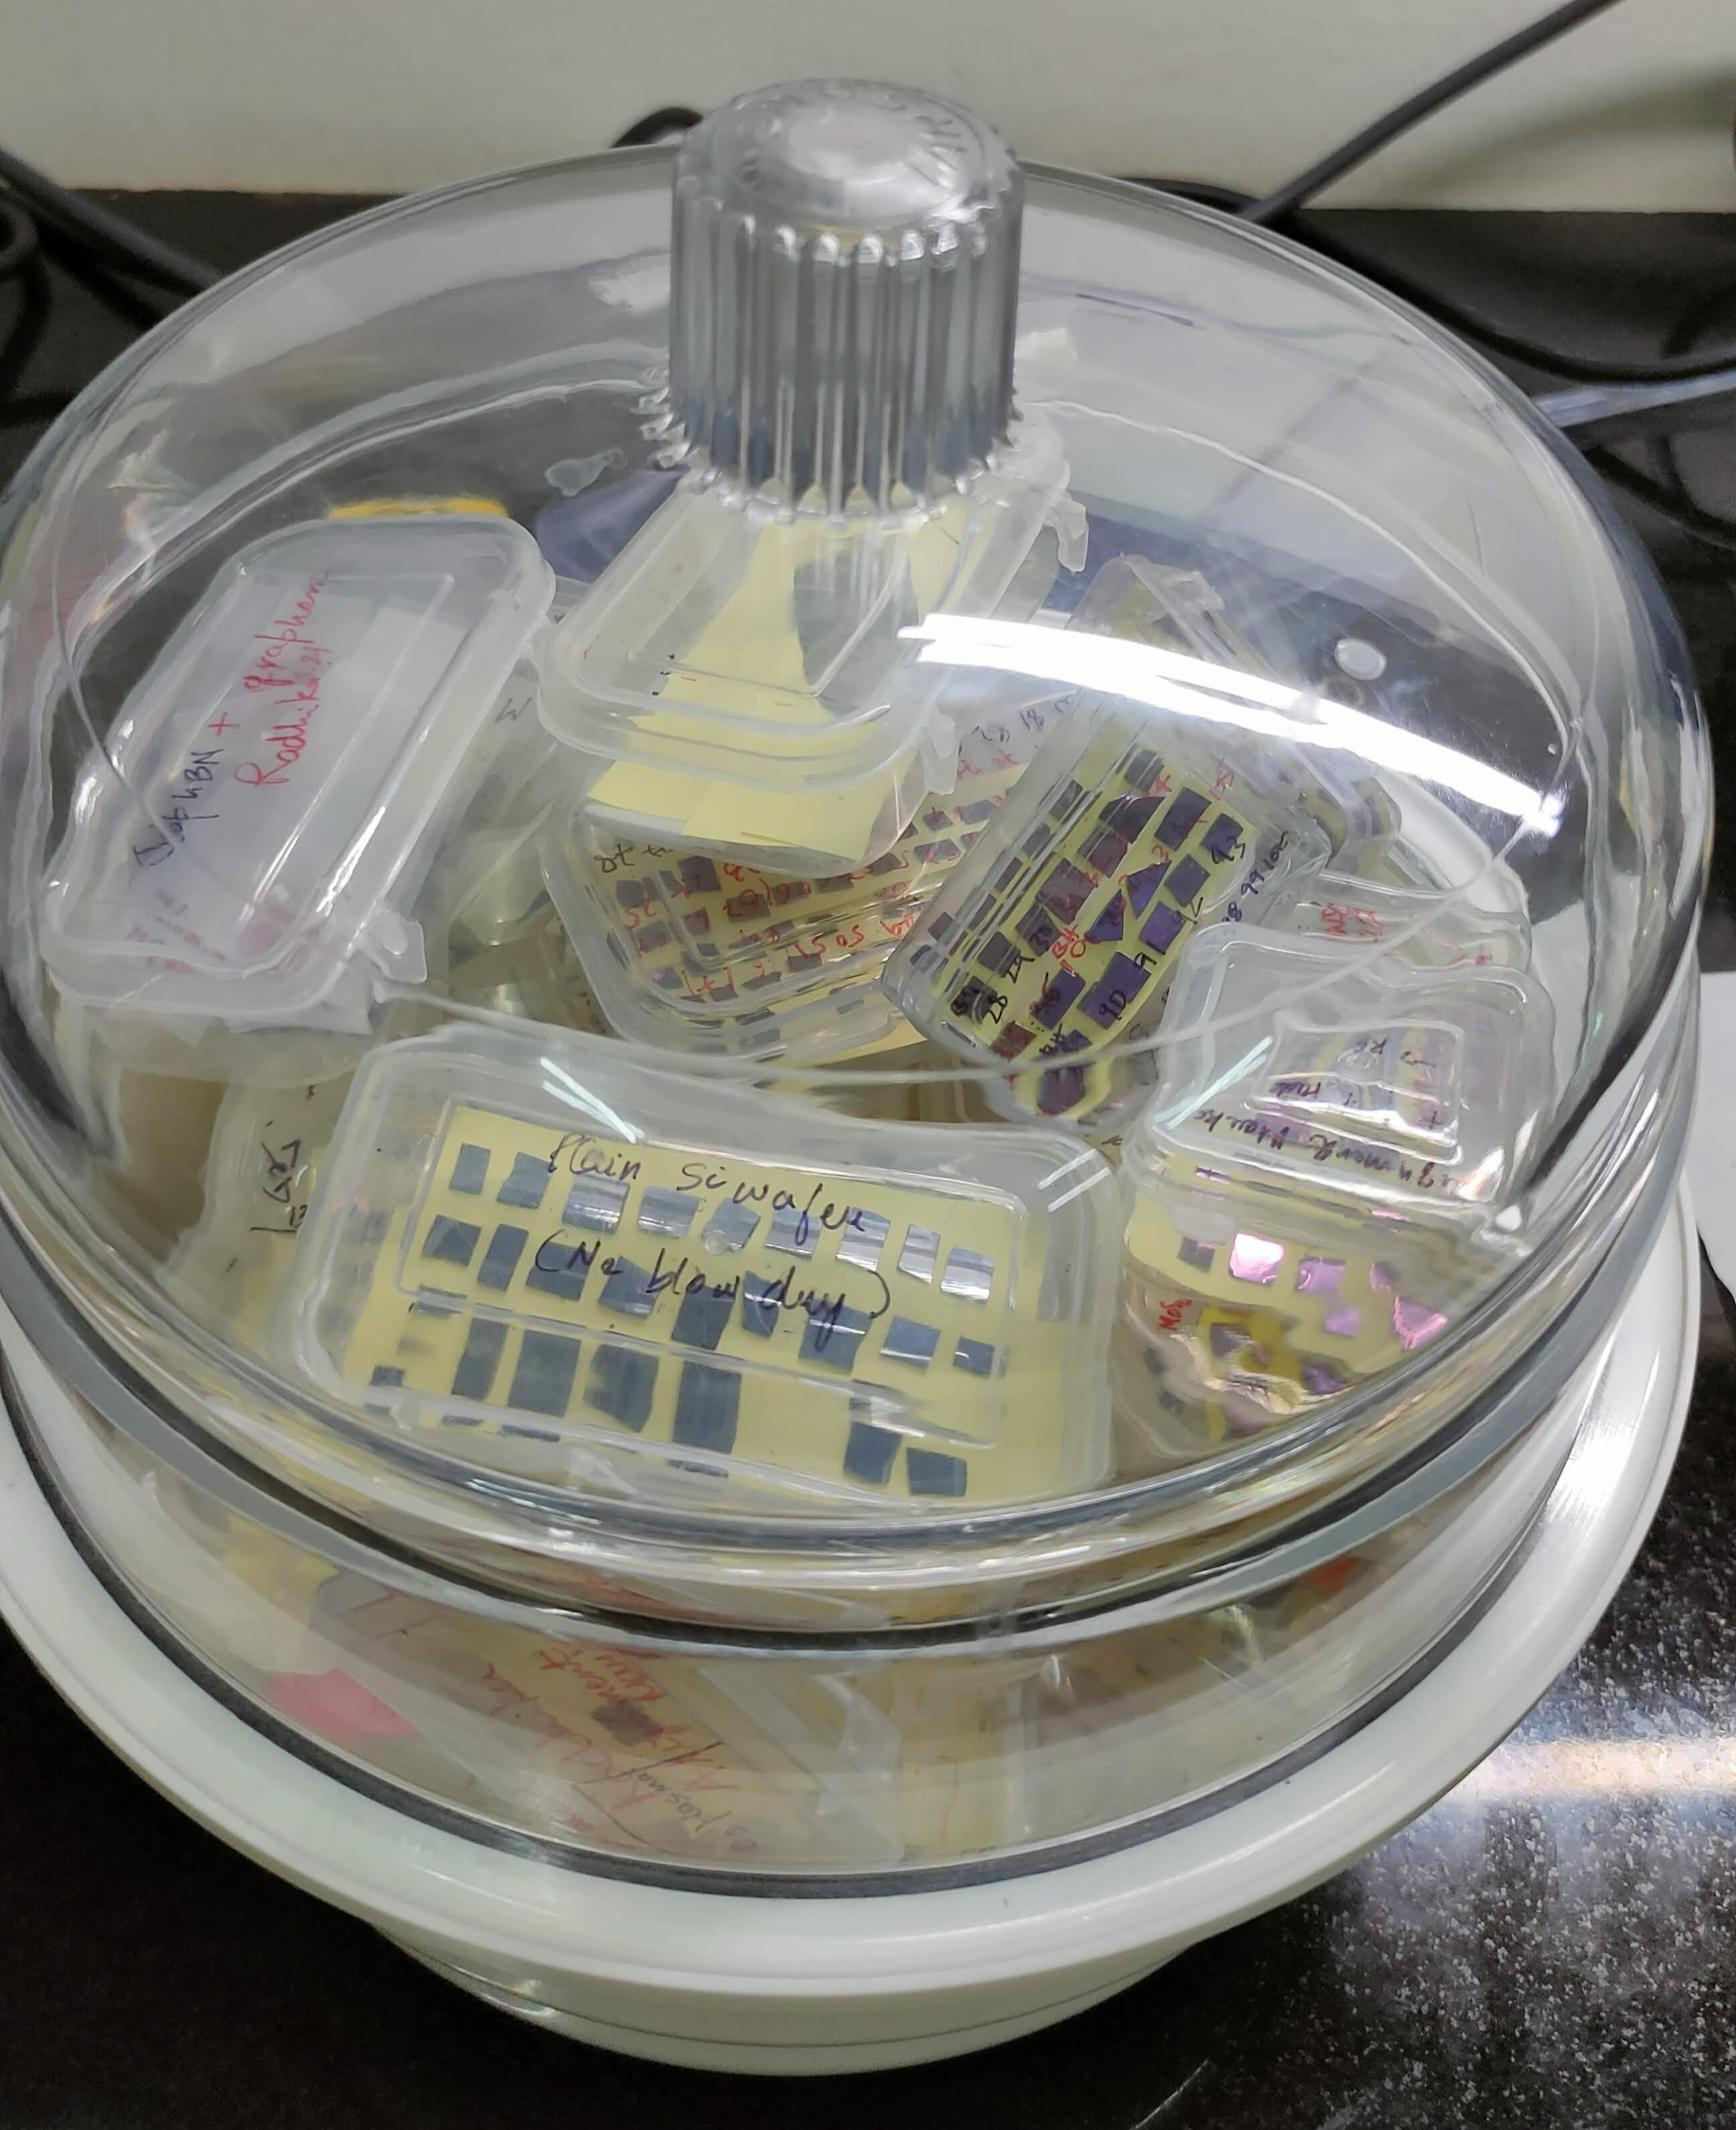
\includegraphics[width=.6\linewidth]{figures/des}
		\caption{A desicator at lab containing boxes that store empty wafers, substrates with flakes and stacks, tapes and devices.}
		\label{fig:des}
	\end{subfigure}
\end{figure}

\section{Flake selection}

\subsection{Optical microscope}

The first thing that is done after the exfoliation of flakes is to check them under optical microscope. The lab has an optical microscope (see fig. \ref{fig:micro}) that has magnifications, 1.25x, 5x, 10x, 50x and 100x.

\begin{figure}[H]
	\centering
	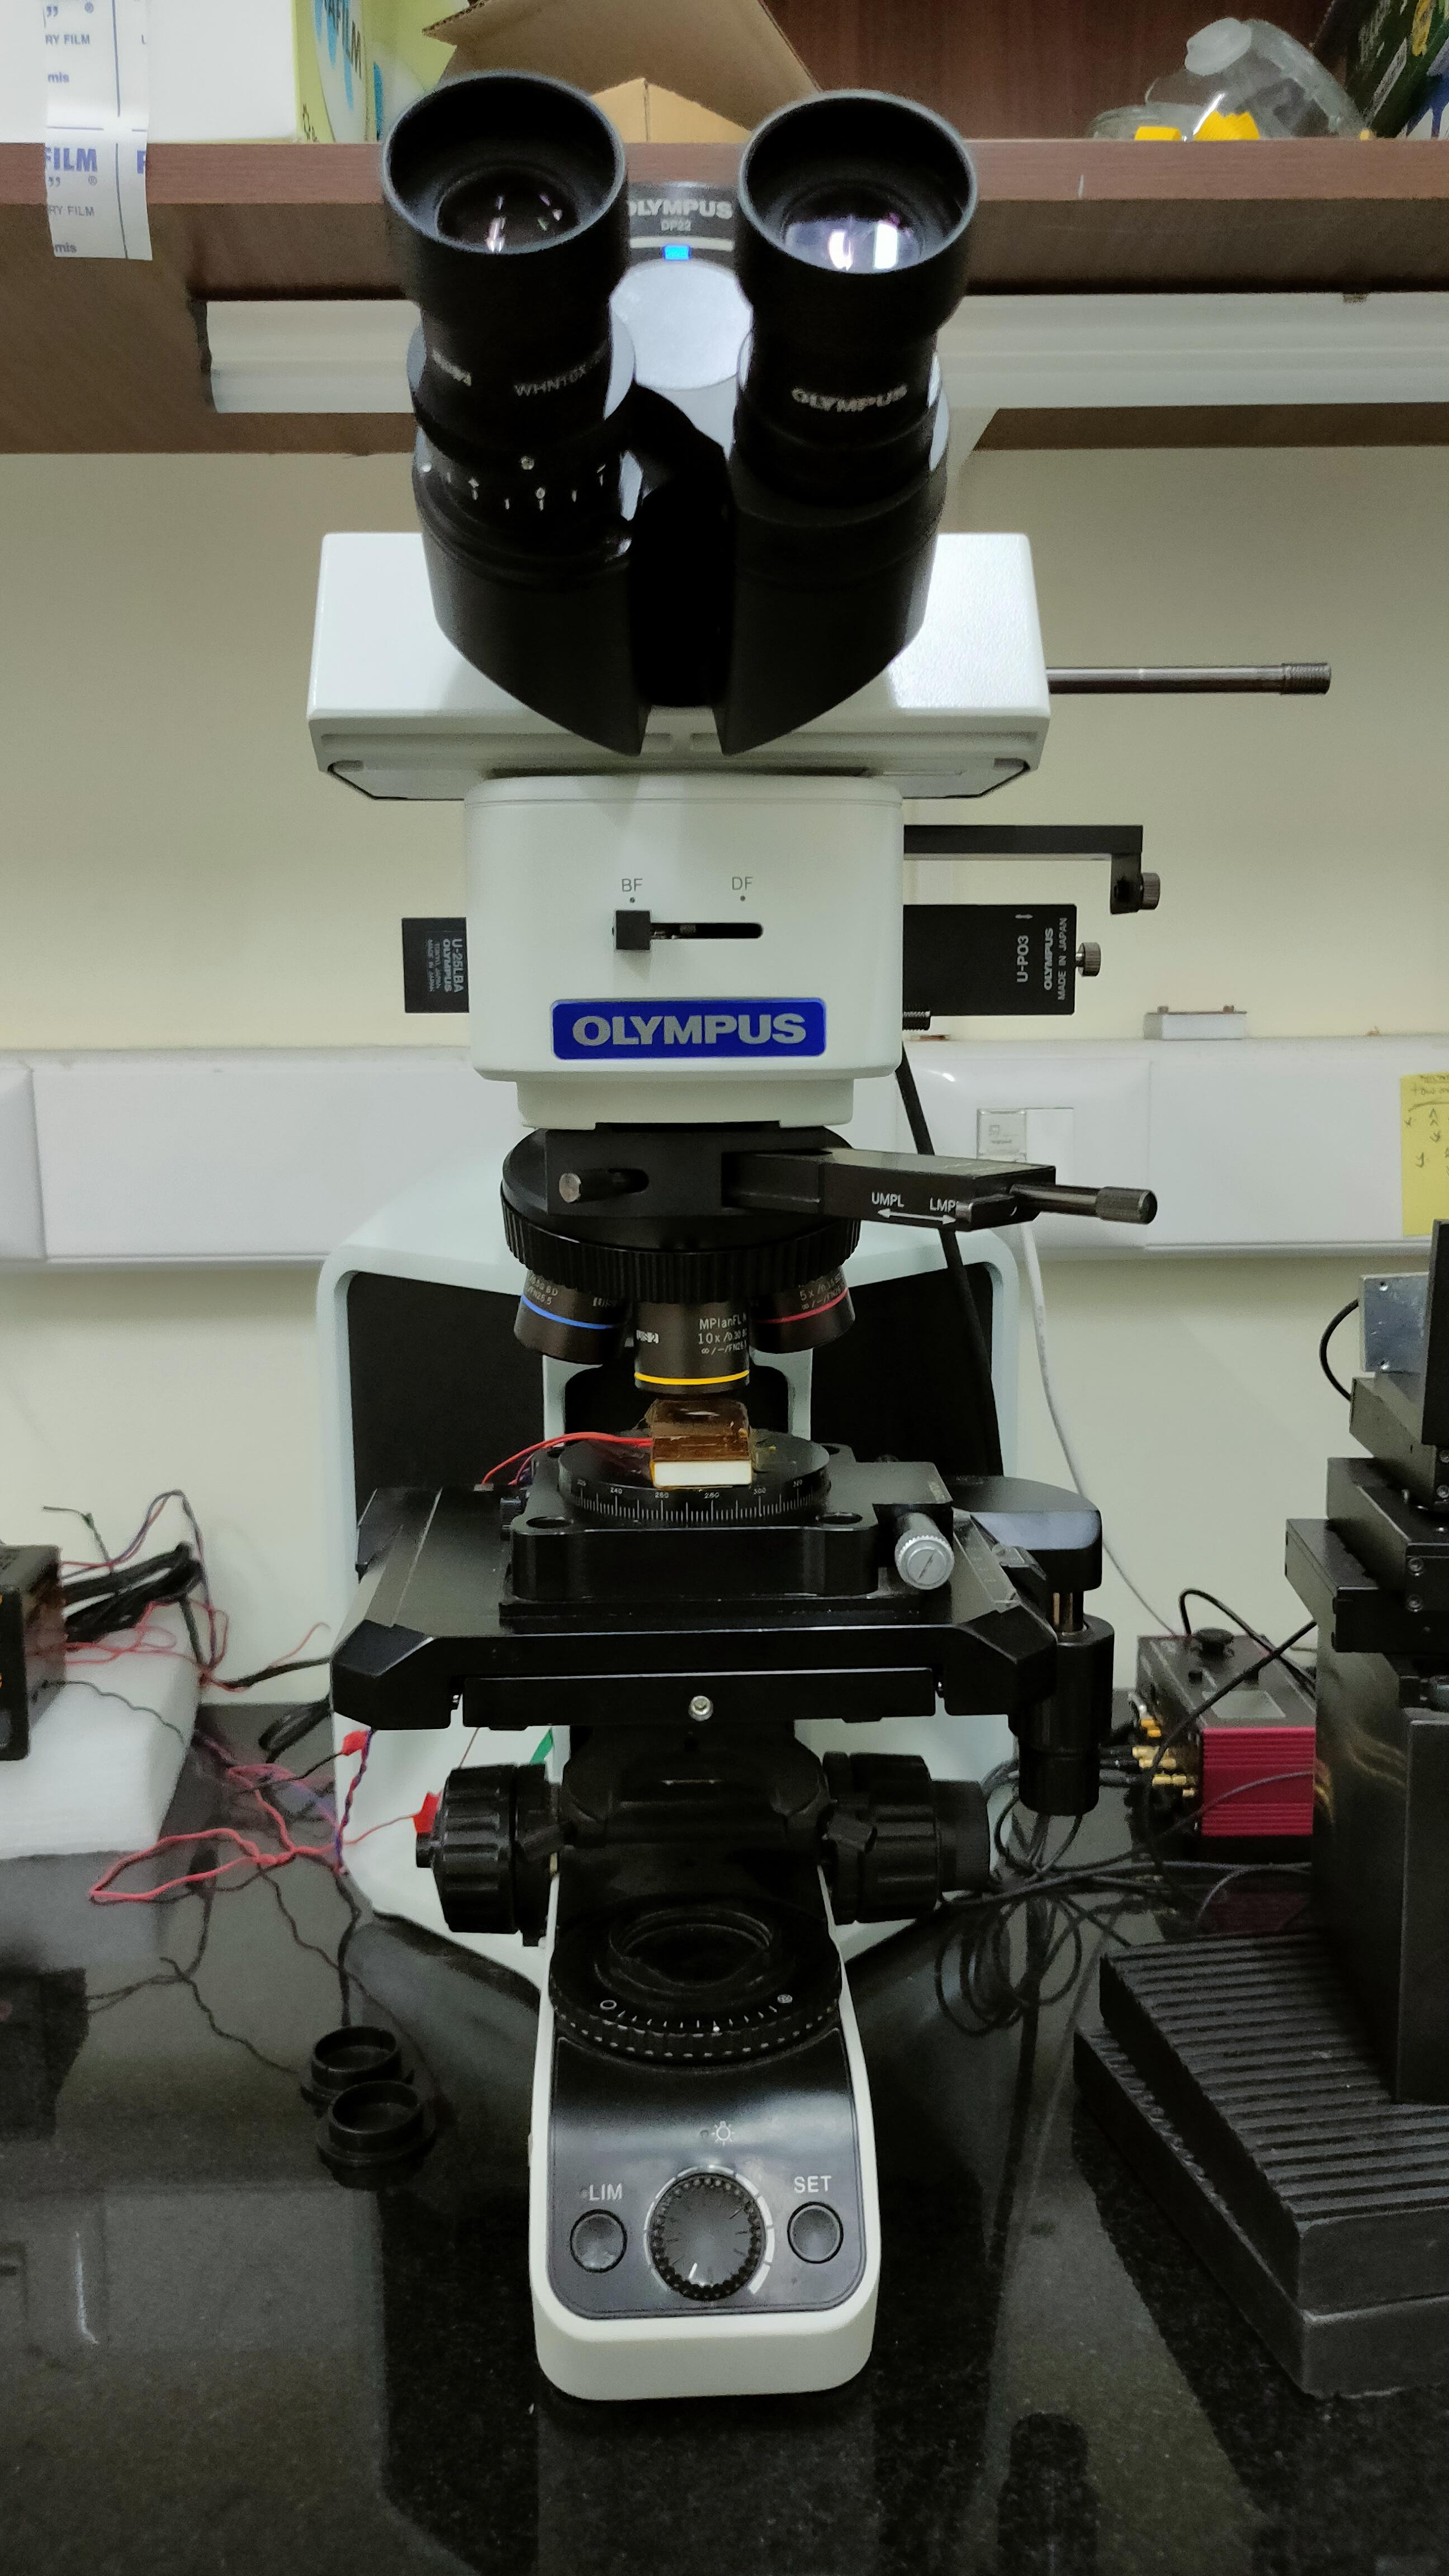
\includegraphics[width=0.5\linewidth]{figures/micro.jpg}
	\caption{Optical microscope at the lab used to find the flakes.}
	\label{fig:micro}
\end{figure}

The colour of the flakes under the microscope depends on the thickness of the flake. As the thickness increases, the colour of the flake changes in the following order for both graphene and hBN: less saturated violet, violet, dark violet, dark blue, light blue, green, pink, yellow (see fig. \ref{fig:thickness}). Monolayers are similar in colour to tape residues, are very faint and hard to find. Hence, when checking a substrate for flakes, the magnification is set to 50x. While searching for thin flakes, like monolayer graphene or few-layered hBN, flakes that are close to some reference thick flakes or attached to them are preferred, as they would be easy to handle during transfer. Also, the size of the flakes should be big enough to make stacks and devices. The optical scans of the flakes are saved at varying magnification, which are used to find the flakes during Raman spectroscopy and AFM.

\begin{figure}[H]
	\centering
	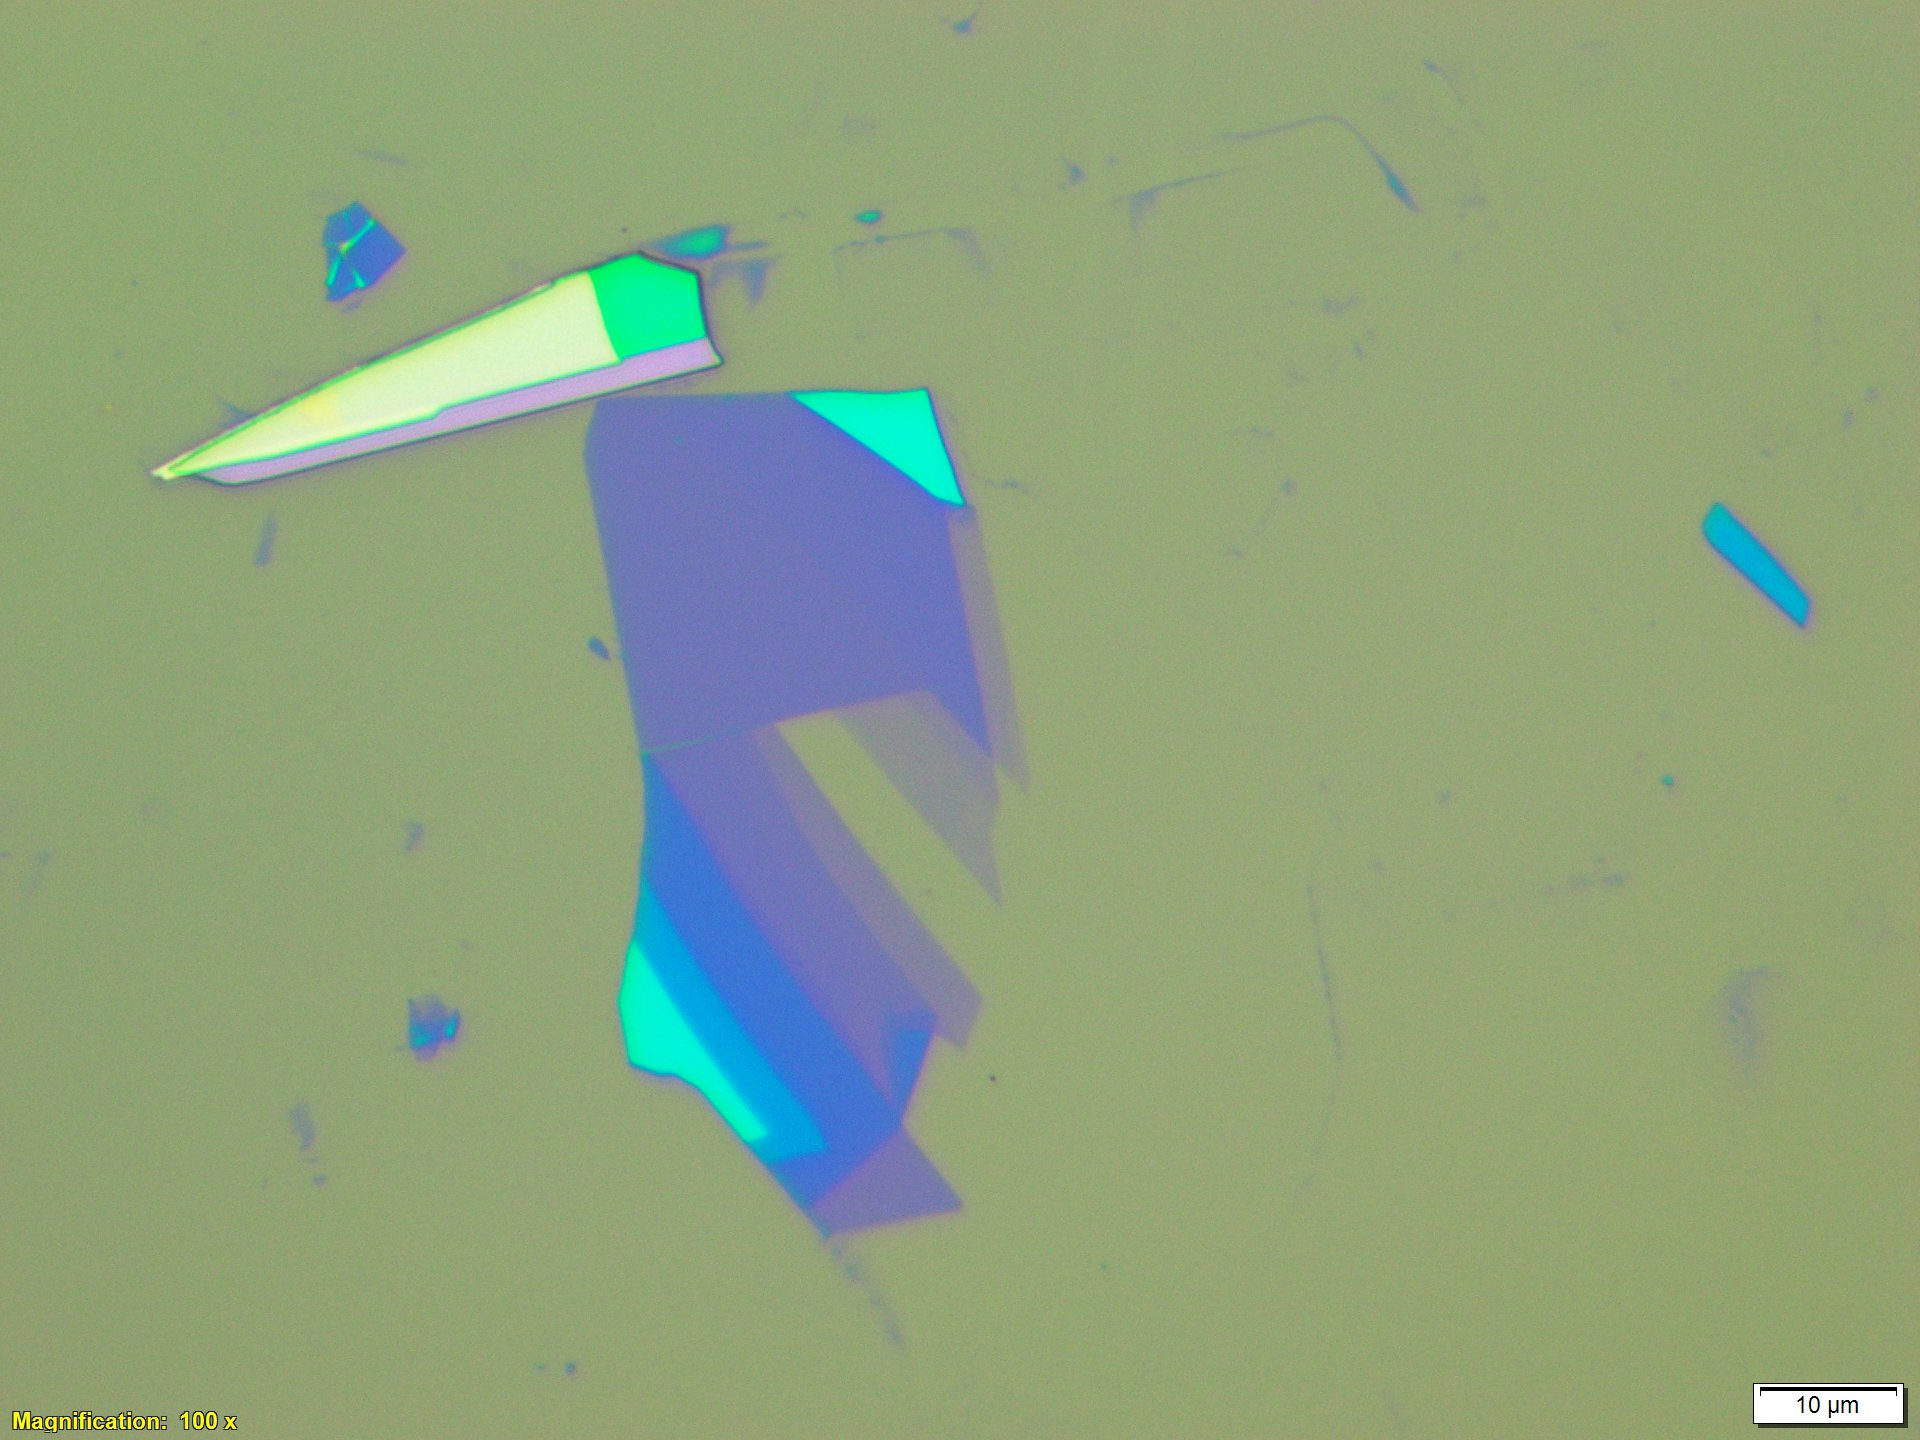
\includegraphics[width=0.6\linewidth]{figures/thickness.jpg}
	\caption{hBN flake showing regions with varying thickness.}
	\label{fig:thickness}
\end{figure}

\subsection{Raman spectroscopy}

Raman spectroscopy is an essential part of graphene research. It is used to determine the number of layers and their orientation. It is also used to probe the effects of perturbations like electric field, magnetic field, strain, disorder, functional groups and doping. 

In graphene, the Stokes phonon energy shift caused by laser excitation creates two main peaks in the Raman spectrum: a primary in-plane vibrational mode, G (1580 cm-1), and a second-order overtone of a different in-plane vibration [D (1350 cm-1)], 2D (2690 cm-1). \cite{Wang_2014} D peak is observed only at the sample edge as there aren't significant number of defects in the center of the graphene layers. \cite{Ferr}

\begin{figure}[H]
	\centering
	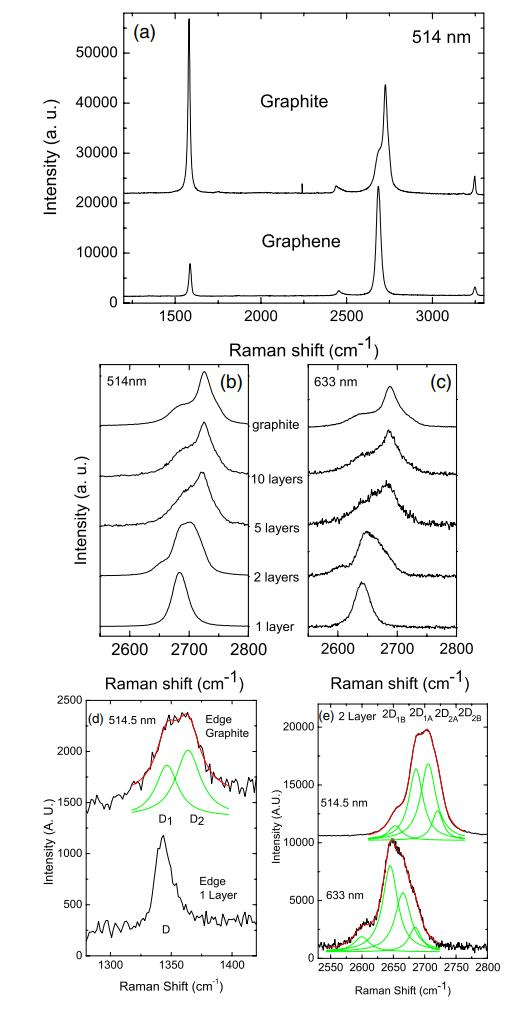
\includegraphics[width=0.7\linewidth]{figures/raman}
	\caption{ (a) Raman spectra of single layer graphene and bulk graphite at 514 nm showing G peak (left) and 2D peak (right). (b,c) Evolution of Raman spectra at 514 nm with number of graphene layers at 514 nm and 633 nm. (d) D band at the edge of single layer graphene and bulk graphite at 514 nm. (e) The four components of the 2D band in 2 layer graphene at 514 and 633 nm.  Figure adapted from \cite{Ferr}}
	\label{fig:raman}
\end{figure}

On increasing the number of graphene layers, the interaction forces between the AB-stacked graphene lead to a change in the spectrum from that of monolayer graphene. The 2D peak splits into an increasing number of modes that combine to give a wider, shorter and higher frequency peak (see fig. \ref{fig:raman}). Hence, the layer number can be identified from the intensity ratio and the number of peaks needed to fit the 2D peak, for example, bilayer graphene needs four Lorentzian fits arising due to four different phonon-assisted intervalley transitions. \cite{Ferr} In general, for monolayer graphene 2D peak is more intense than G peak, whereas for bilayer, both the peaks show similar intensities. Rotationally disordered (decoupled) multilayer graphene, however, can still have a single intense 2D peak regardless of thickness, \cite{LESPADE1984375} though its position and FWHM can depend on the number of layers. \cite{Ferr}

Raman is also used to determine the number of hBN layers in a flake. hBN exhibits a characteristic peak due to the $E_2g$ phonon mode and similar to the G peak in graphene. The Raman peak occurs at $\approx1366 cm^{-1}$, and the peak intensity decreases as the number of layers decreases. \cite{Peter} For monolayer hBN, peak intensity is about 50 times smaller than for graphene’s G peak under the same measurement conditions. The integrated intensity for the hBN peak is proportional to N with high accuracy for the first several layers (see fig. \ref{fig:raman_hbn}).

\begin{figure}[H]
	\centering
	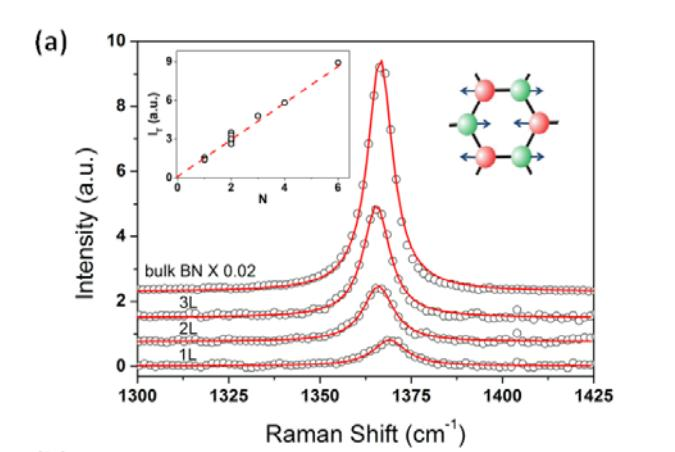
\includegraphics[width=0.7\linewidth]{figures/raman_hbn}
	\caption{Raman spectra of hBN of varying thickness. The left inset show changes in integrated intensity with the number of layers N. The right picture illustrates the phonon mode responsible for the Raman peak. Figure adapted from \cite{Peter}}
	\label{fig:raman_hbn}
\end{figure}

\subsection{Atomic force microscopy}

Atomic force microscopy (AFM) is a type of scanning probe microscopy (SPM). It has resolution in the order of fractions of a nanometer, which is useful in mapping the thickness variations in the flakes we use. It is also helpful in determining how clean the flakes are and if they can be used to make stacks. AFM can image almost any type of surface, including polymers, ceramics, composites, glass, and biological samples. This is because, atomic forces are used to map the tip-sample interaction. AFM has a feedback loop using the laser deflection to control the force and tip position. A laser is reflected from the back of a cantilever that includes the AFM tip. As the tip interacts with the surface, the laser position on the photodetector is used in the feedback loop to track the surface for imaging.

Fig. \ref{fig:afm} shows AFM imaging of hBN flake to determine the thickness, evenness and cleanliness. It can be seen that the thickness of the flake shown is 5nm. From the graph, it is clear that the flake is even in the region selected and
it is clean.

\begin{figure}[H]
	\centering
	\includegraphics[width=\linewidth]{figures/afm.jpg}
	\caption{AFM of 5nm hBN flake. Top right: Optical image of the flake. Top left: AFM mapping of the flake, to find cleanliness. Bottom: Thickness of hBN flake as a function of position taken along the line shown in the top left figure. }
	\label{fig:afm}
\end{figure}

\section{Stamp creation}

Stacks of graphene and hBN are created by putting them on top of each other, using the Pickup and Transfer process. This process involves the use of polymer stamps that can stick to a flake and pick it up. The stamp consists of a coverslip with PPC (Polypropylene carbonate) or PC (Poly(Bisphenol A carbonate)) on hemispherical PDMS (Polydimethylsiloxane). The first step is to make the PDMS coverslips. The protocol is as follows:
\begin{enumerate}
	\item Sonicate coverslips in acetone, wash with IPA and blowdry in $N_2$. Fig. \ref{fig:soni} shows the sonicator used at the lab.
	\item Bake the coverslips for 5 minutes at 150 $^{\circ}$C to remove moisture.
	\item Mix 10 parts PDMS with 1 part curing agent on a clean glass slide using a clean toothpick.
	\item Put PDMS onto the coverslips using a toothpick, picking up some PDMS mixture by holding the toothpick vertically.
	\item Bake the coverslips at 150 $^{\circ}$C for 30 min. A coverslip with PDMS on it looks as shown in fig. \ref{fig:pdms}
\end{enumerate}

\begin{figure}[H]
	\centering
	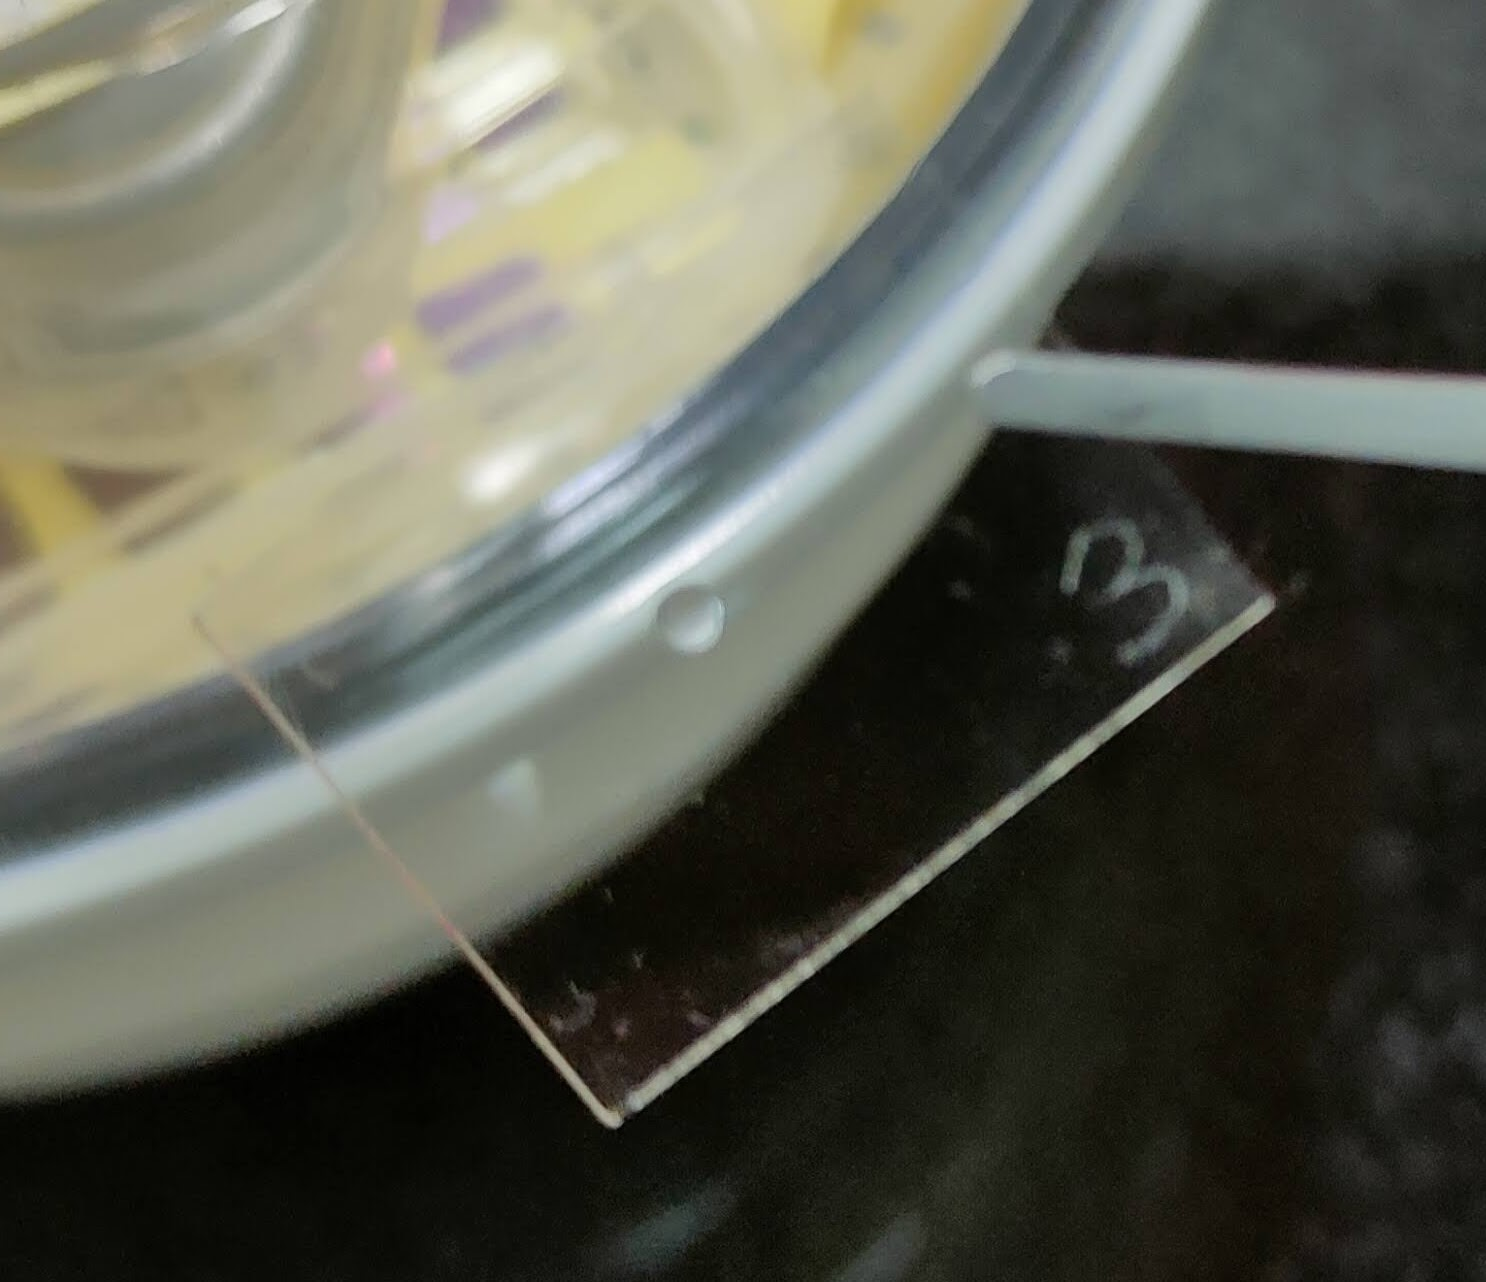
\includegraphics[width=0.4\linewidth]{figures/pdms}
	\caption{A coverslip with PDMS on it.}
	\label{fig:pdms}
\end{figure}

A layer of PPC or PC is now added on PDMS that is used to pickup the flakes. The steps for this are:
\begin{enumerate}
	\item Put a drop or two of PPC (15 percent PPC in anisole) or PC (6 percent PC in Chloroform) on PDMS coverslip using a dropper. Use glass dropper for PC.
	\item Spin coat it at 3000rpm for 30s by attaching the coverslip to the spin coater with a double-sided tape. Fig. \ref{fig:spco} shows the spin coater used at lab.
	\item Keep the coverslip immediately on the hot plate to bake at 70 $^o$C for 10 mins.
\end{enumerate}

\begin{figure}[H]
	\centering
	\begin{subfigure}{.5\linewidth}
		\centering
		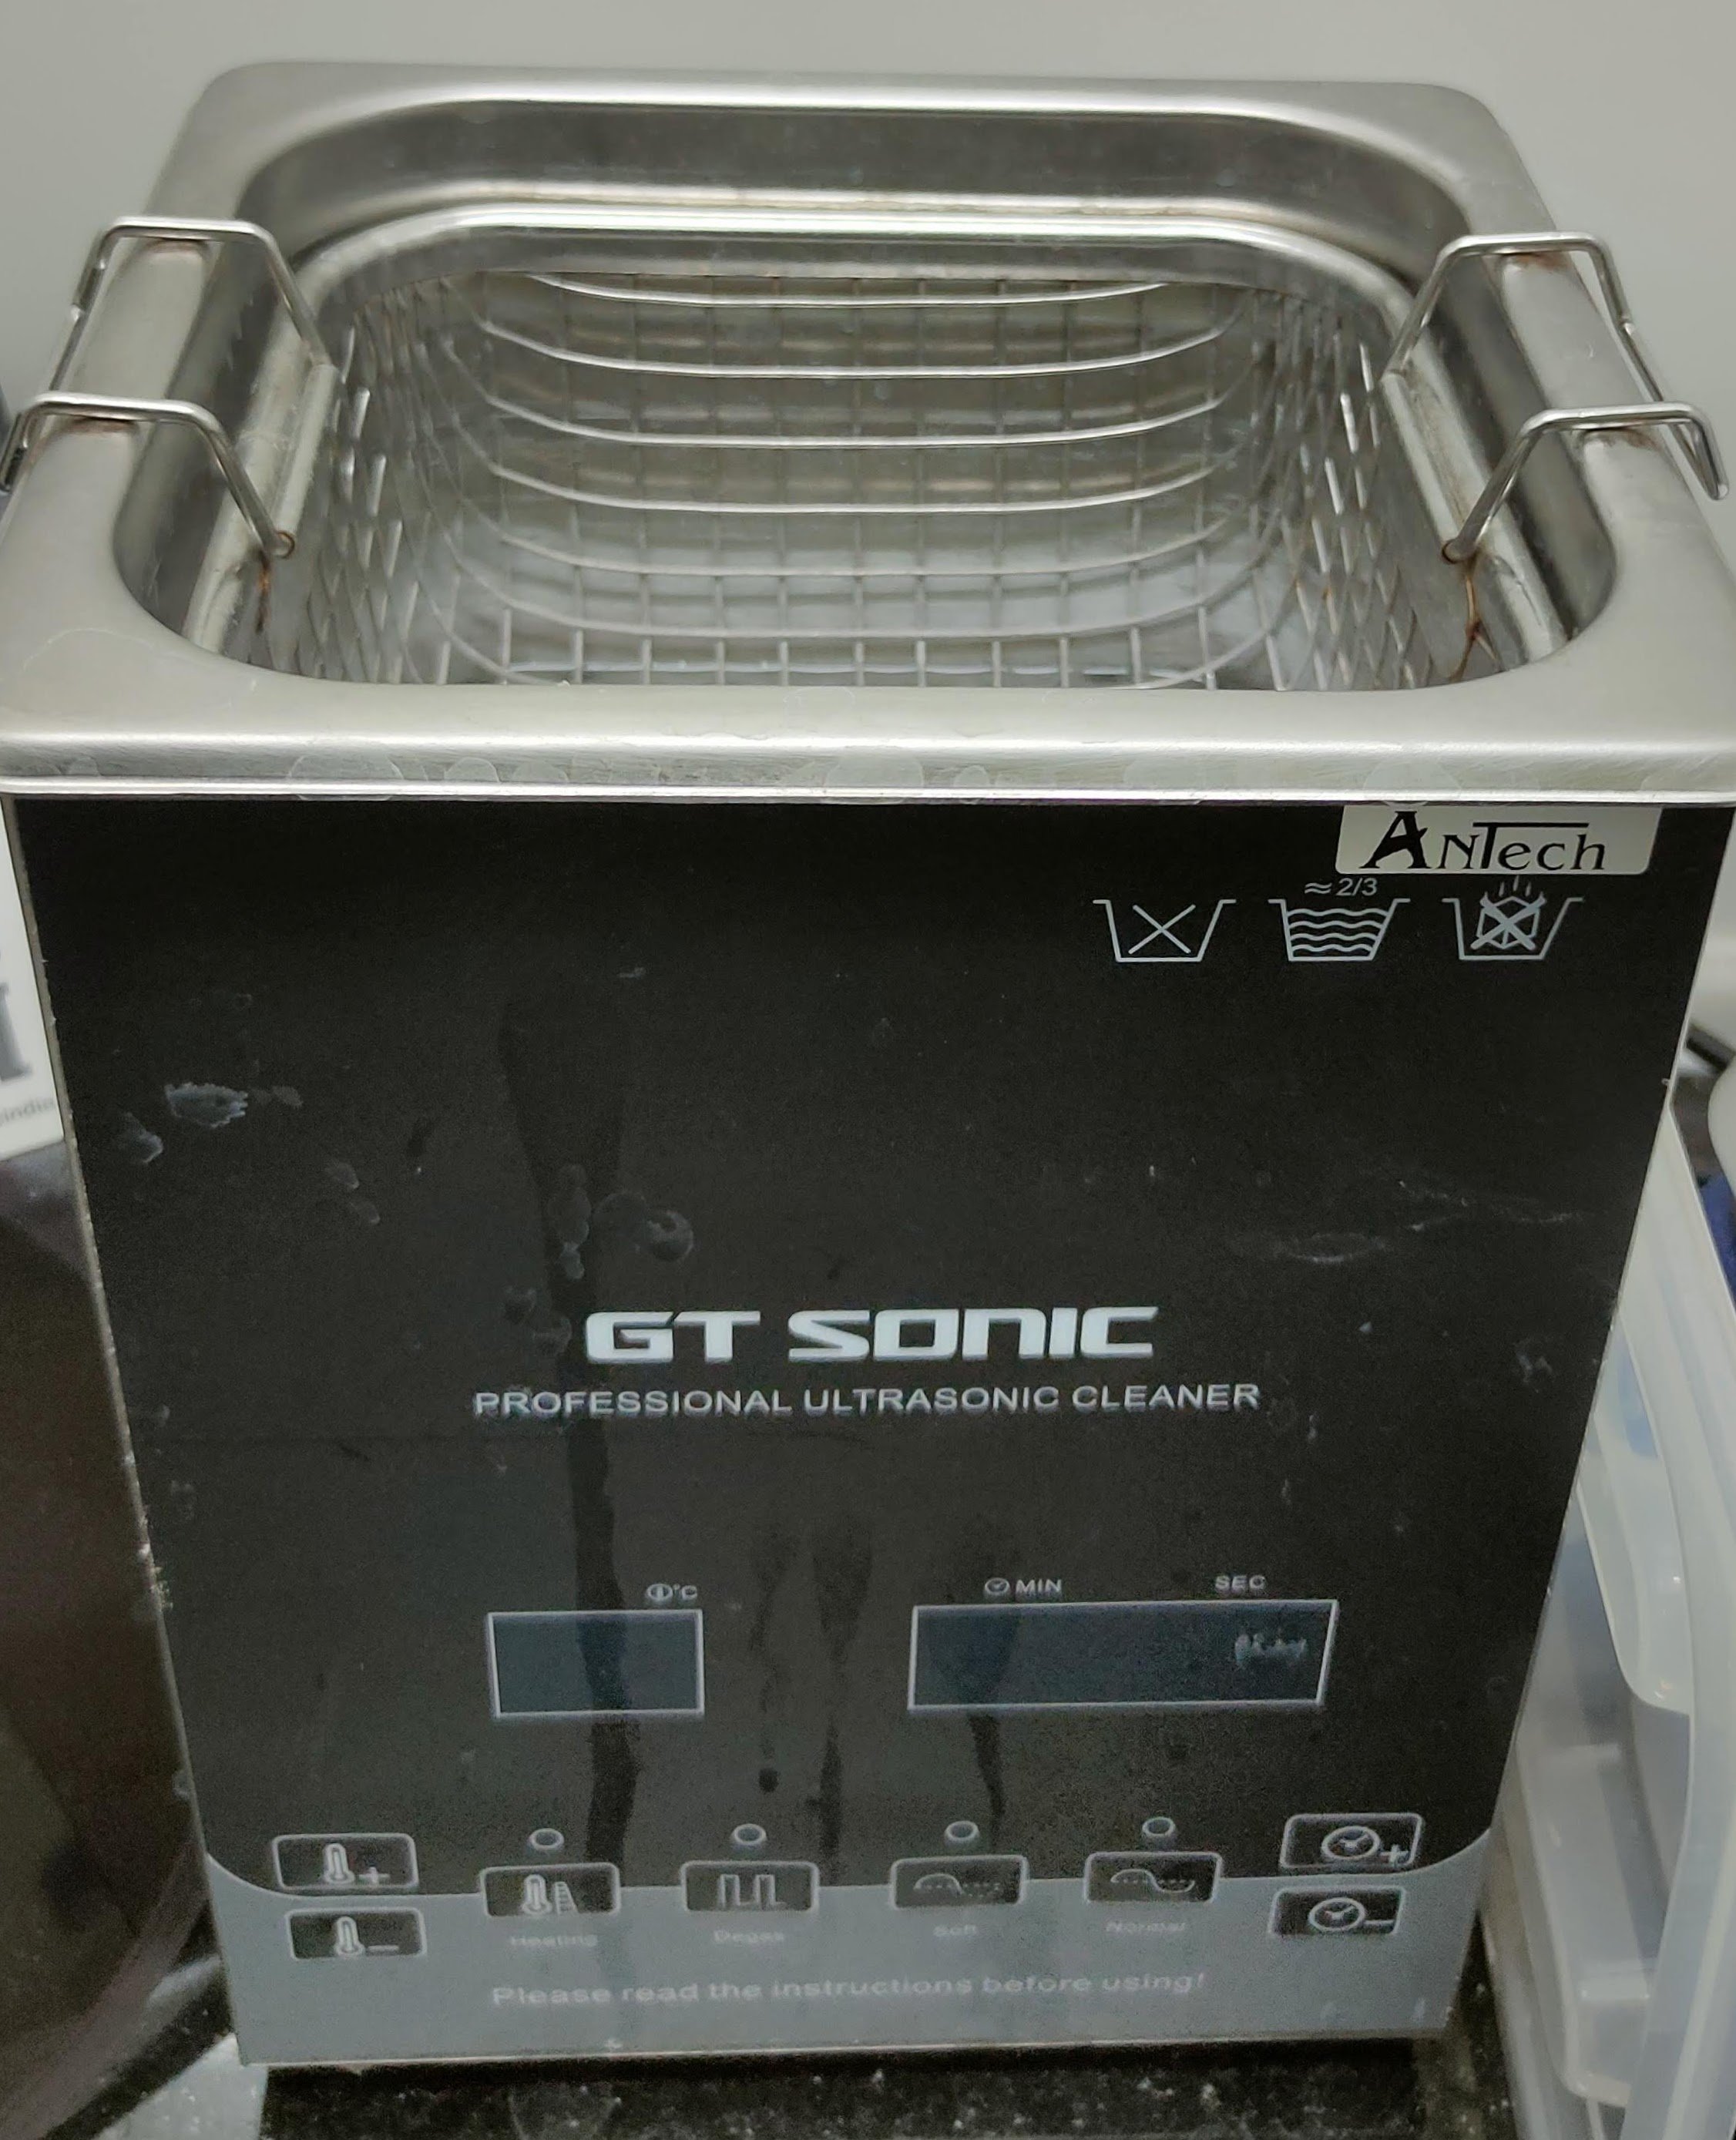
\includegraphics[width=0.6\linewidth]{figures/soni}
		\caption{Sonicator (Ultrasound cleaner) at lab}
		\label{fig:soni}
	\end{subfigure}%
	\begin{subfigure}{.5\linewidth}
		\centering
		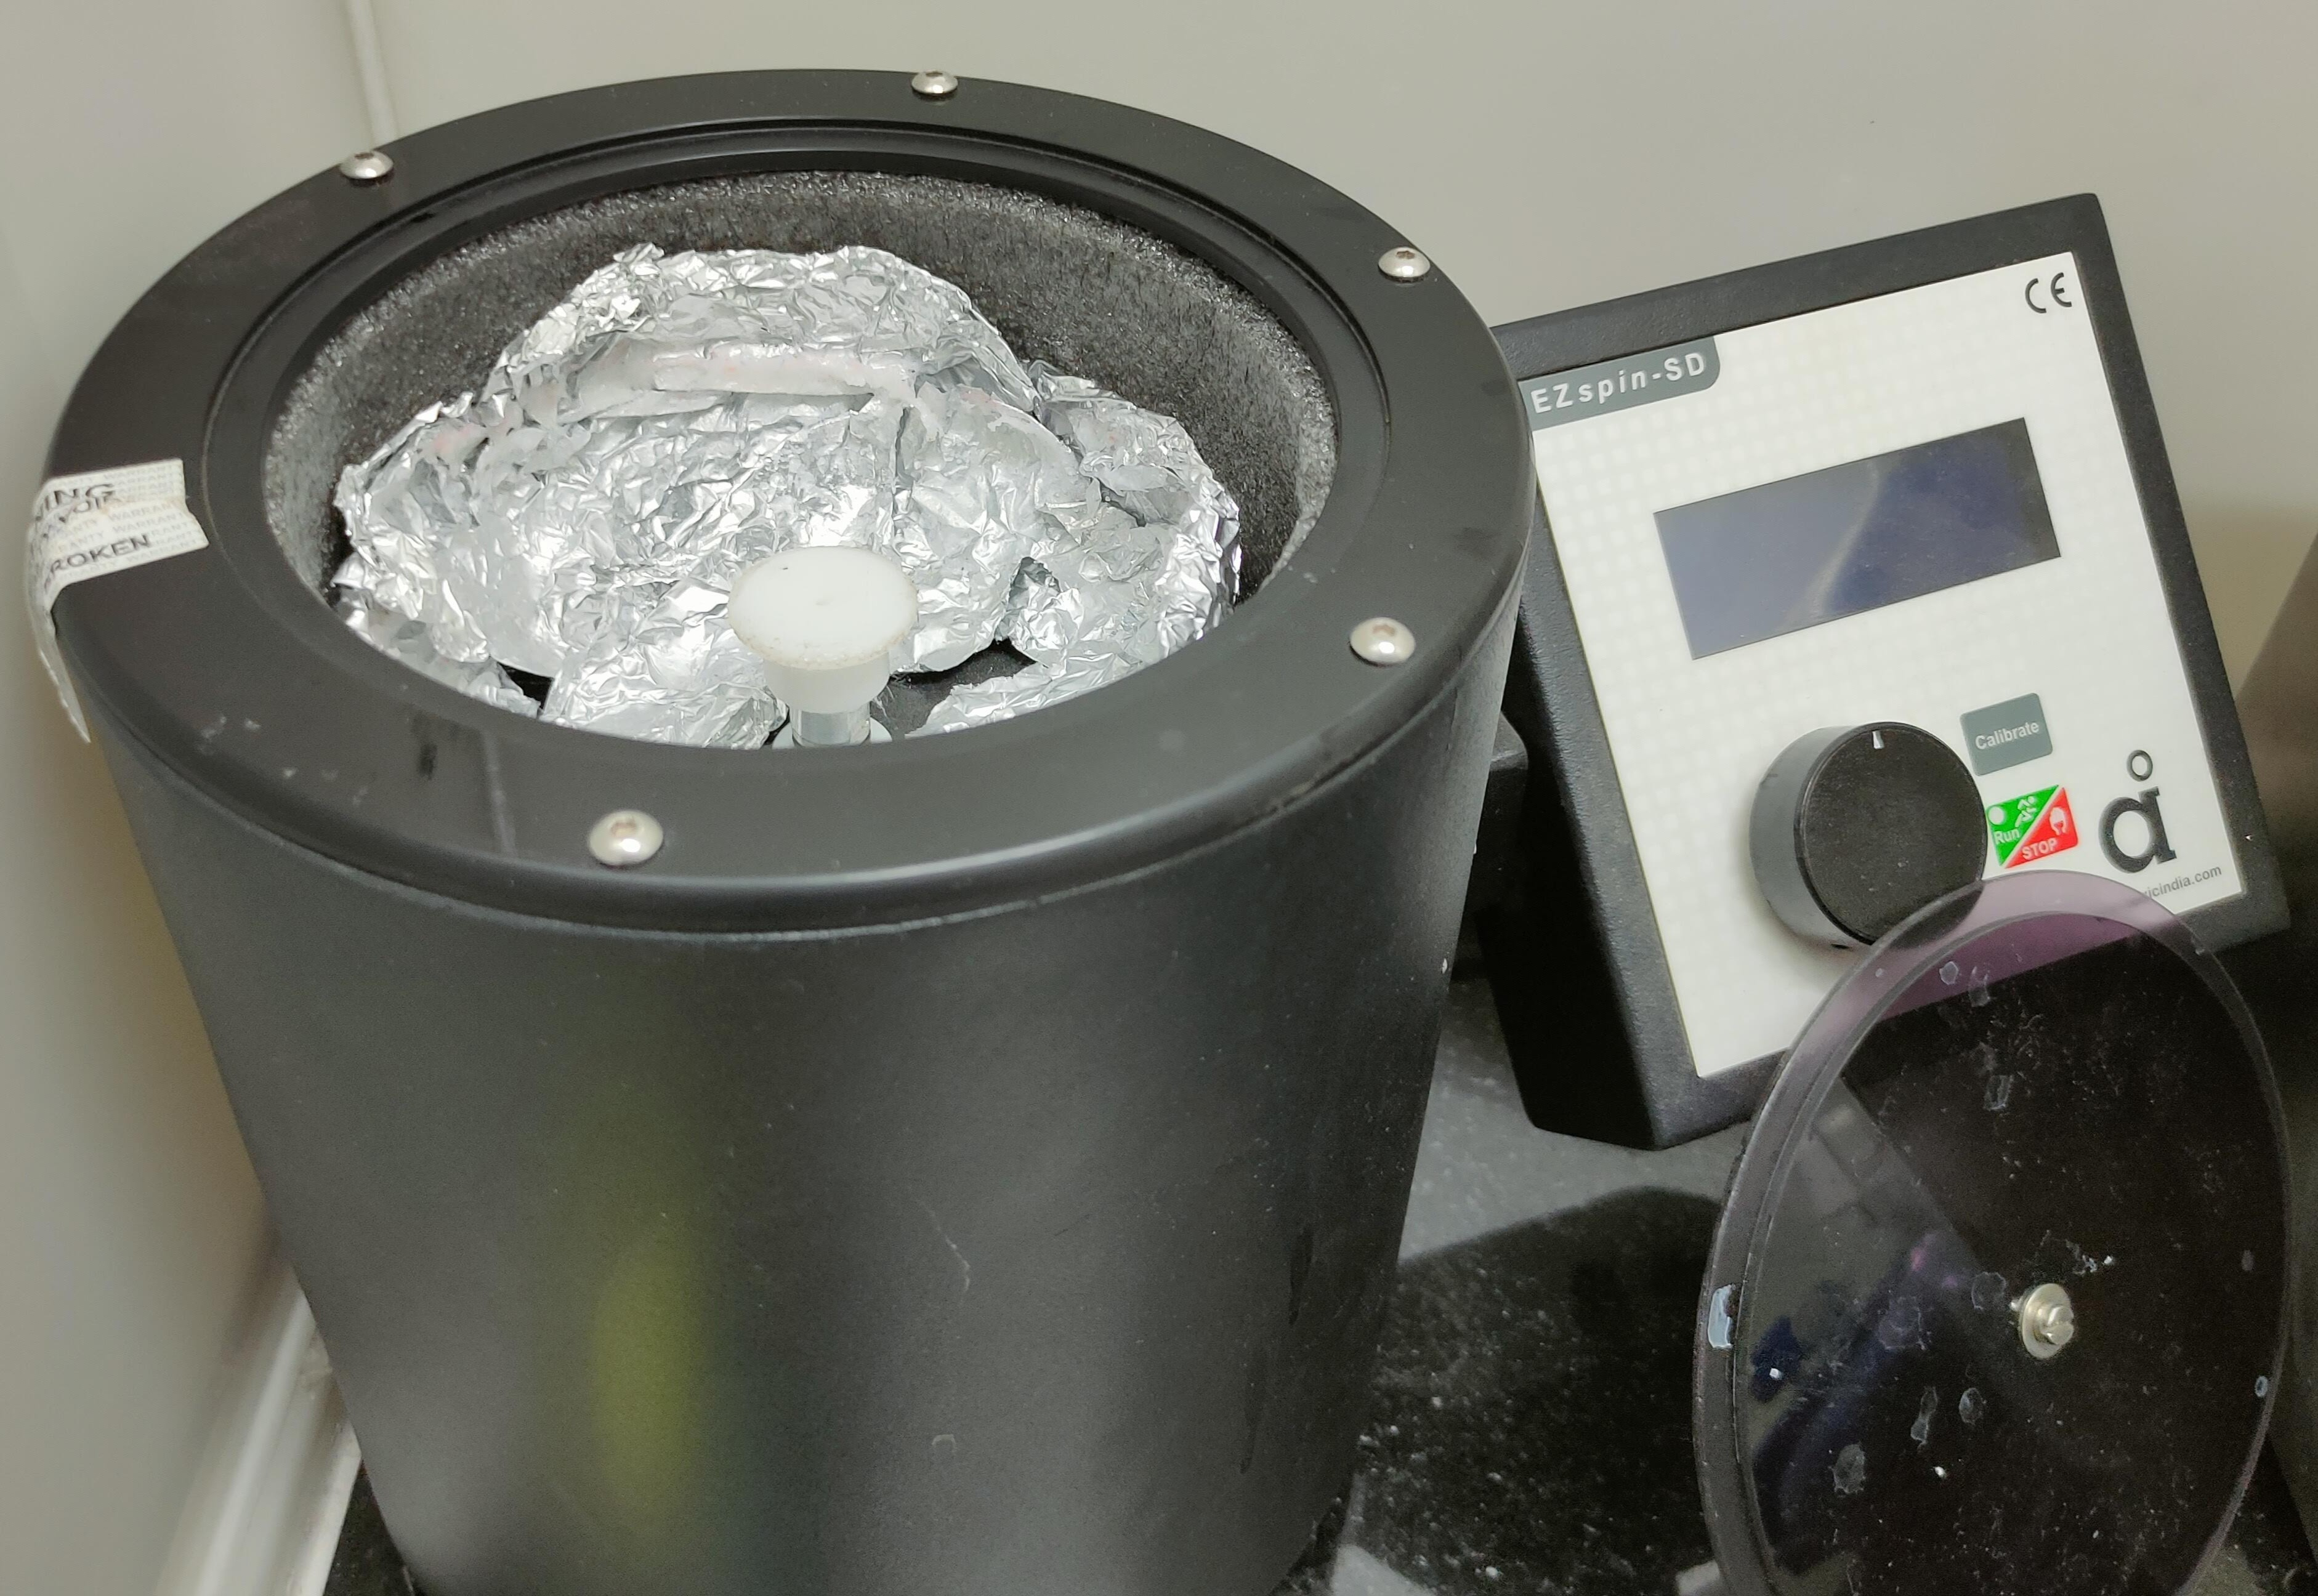
\includegraphics[width=0.8\linewidth]{figures/spco}
		\caption{Spin coater at lab}
		\label{fig:spco}
	\end{subfigure}
	\caption{Sonicator and spin coater at lab.}
\end{figure}

PPC or PC solution has to be kept ready before starting stamp making. For making PPC solution: 
\begin{enumerate}
	\item Take a small glass bottle, wash it and heat it at 80 $^o$C for 1hr 30min. \item Measure and transfer 10ml of anisole in the bottle and add 1.5g of PPC crystals in it, making a solution.
	\item Shake the bottle vigorously and leave overnight.
\end{enumerate}
For making PC solution:
\begin{enumerate}
	\item Wash a small glass bottle. 
	\item Measure and transfer 3ml of Chloroform in the bottle and add 0.18g of PC crystals in it.
	\item Leave the bottle overnight.
\end{enumerate}
This coverslip is stuck on the transfer stage using an aluminium plate. This is done with the following steps:
\begin{enumerate}
	\item Keep the coverslip on the metal stick and add EL-9 along the edges of the coverslip using a micropipette.
	\item Bake this at 90 $^{\circ}$C on the hot plate for 2-3 mins.
	\item Attach the aluminium plate to the stage using double-sided tape.
\end{enumerate}

\section{Pickup and transfer process}
\label{section:f}

We now discuss the pickup and transfer process, called the dry transfer technique. \cite{Kim16,Wang614} After the PPC-PDMS and/or PC-PDMS stamp is ready, this process is started in the transfer setup (shown in fig. \ref{fig:tr_set}). PC-PDMS stamp is used for thin hBN transfer and PC-PDMS stamp for everything else. The choice is based on optimisation. Fig. \ref{fig:schematic} and \ref{fig:schematic} show the schematic of pickup and transfer process used to make a tunnel device, discussed in detail below.

\begin{figure}[H]
	\centering
	\begin{subfigure}{\linewidth}
		\centering
		\includegraphics[width=0.9\linewidth]{figures/schematic1}
	\end{subfigure}
	\caption{Schematic of pickup and transfer process used in making twisted bilayer graphene stack for tunneling measurement: Part 1.}
	\label{fig:schematic1}
\end{figure}

\begin{figure}[H]
	\centering
	\begin{subfigure}{\linewidth}
		\centering
		\includegraphics[width=0.8\linewidth]{figures/schematic2}
	\end{subfigure}
	\begin{subfigure}{\linewidth}
		\centering
		\includegraphics[width=0.8\linewidth]{figures/schematic3}
	\end{subfigure}
	\caption{Schematic of pickup and transfer process used in making twisted bilayer graphene stack for tunneling measurement: Part 2.}
	\label{fig:schematic}
\end{figure}

The transfer setup consists of the following parts:
\begin{enumerate}
	\item OSL2 fiber illuminator: provides illumination for the microscope stage
	\item Micro position controller: power source of the rotation stage
	\item PID temperature controller: heats the stage
	\item Regulated DC power supply: provides voltage to the temperature controller
	\item Optical cable: connects illuminator to the microscope
	\item Moticam camera: used to see and capture samples under the microscope
	\item Optical microscope: has 20x magnification with up to 4x zoom
	\item Microscope stage: holds the substrate and has an integrated heater
	\item Motorized twist stage: used in twisted bilayer stack making
	\item Transfer component: contains an aluminium plate and Piezo actuators 
	\item Piezo motor controller: powers Piezo actuators
	
\end{enumerate}

\begin{figure}[H]
	\centering
	\begin{minipage}{.45\linewidth}
		\begin{subfigure}[t]{0.9\textwidth}
			\centering
			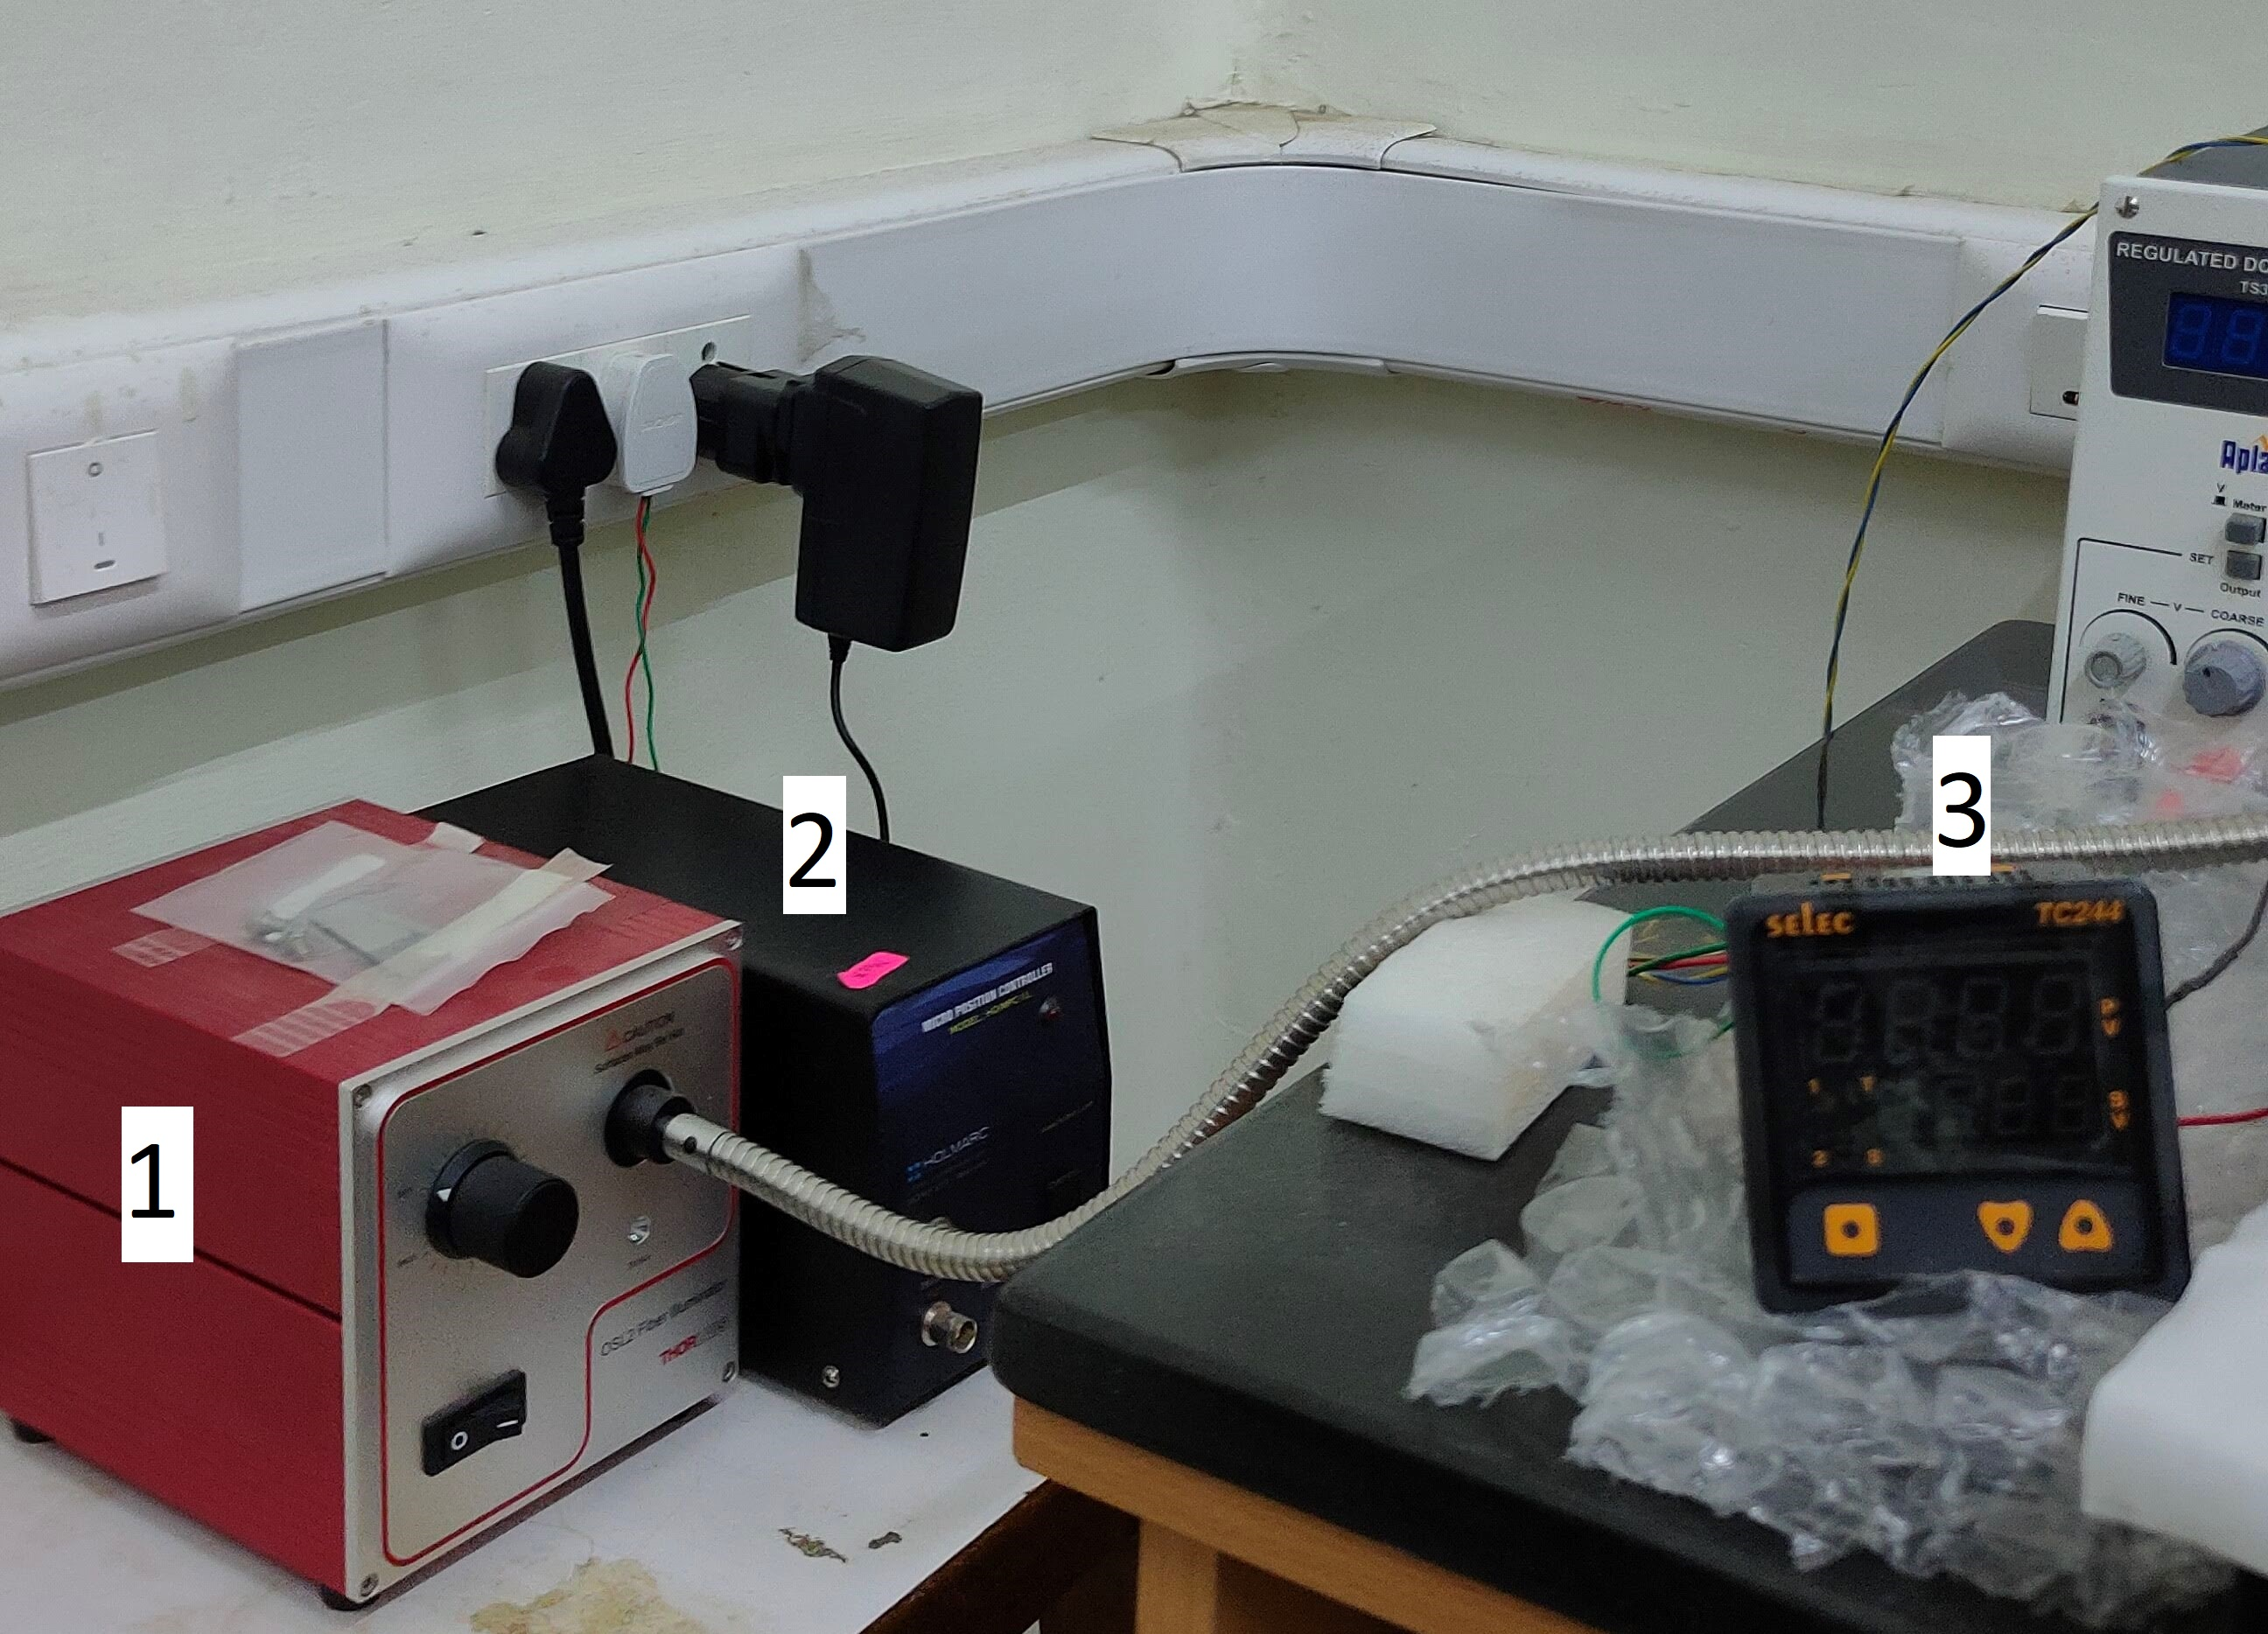
\includegraphics[width=\textwidth]{figures/trset1.jpg}
		\end{subfigure}
		\\
		\\
		\begin{subfigure}[b]{0.9\textwidth}
			\centering
			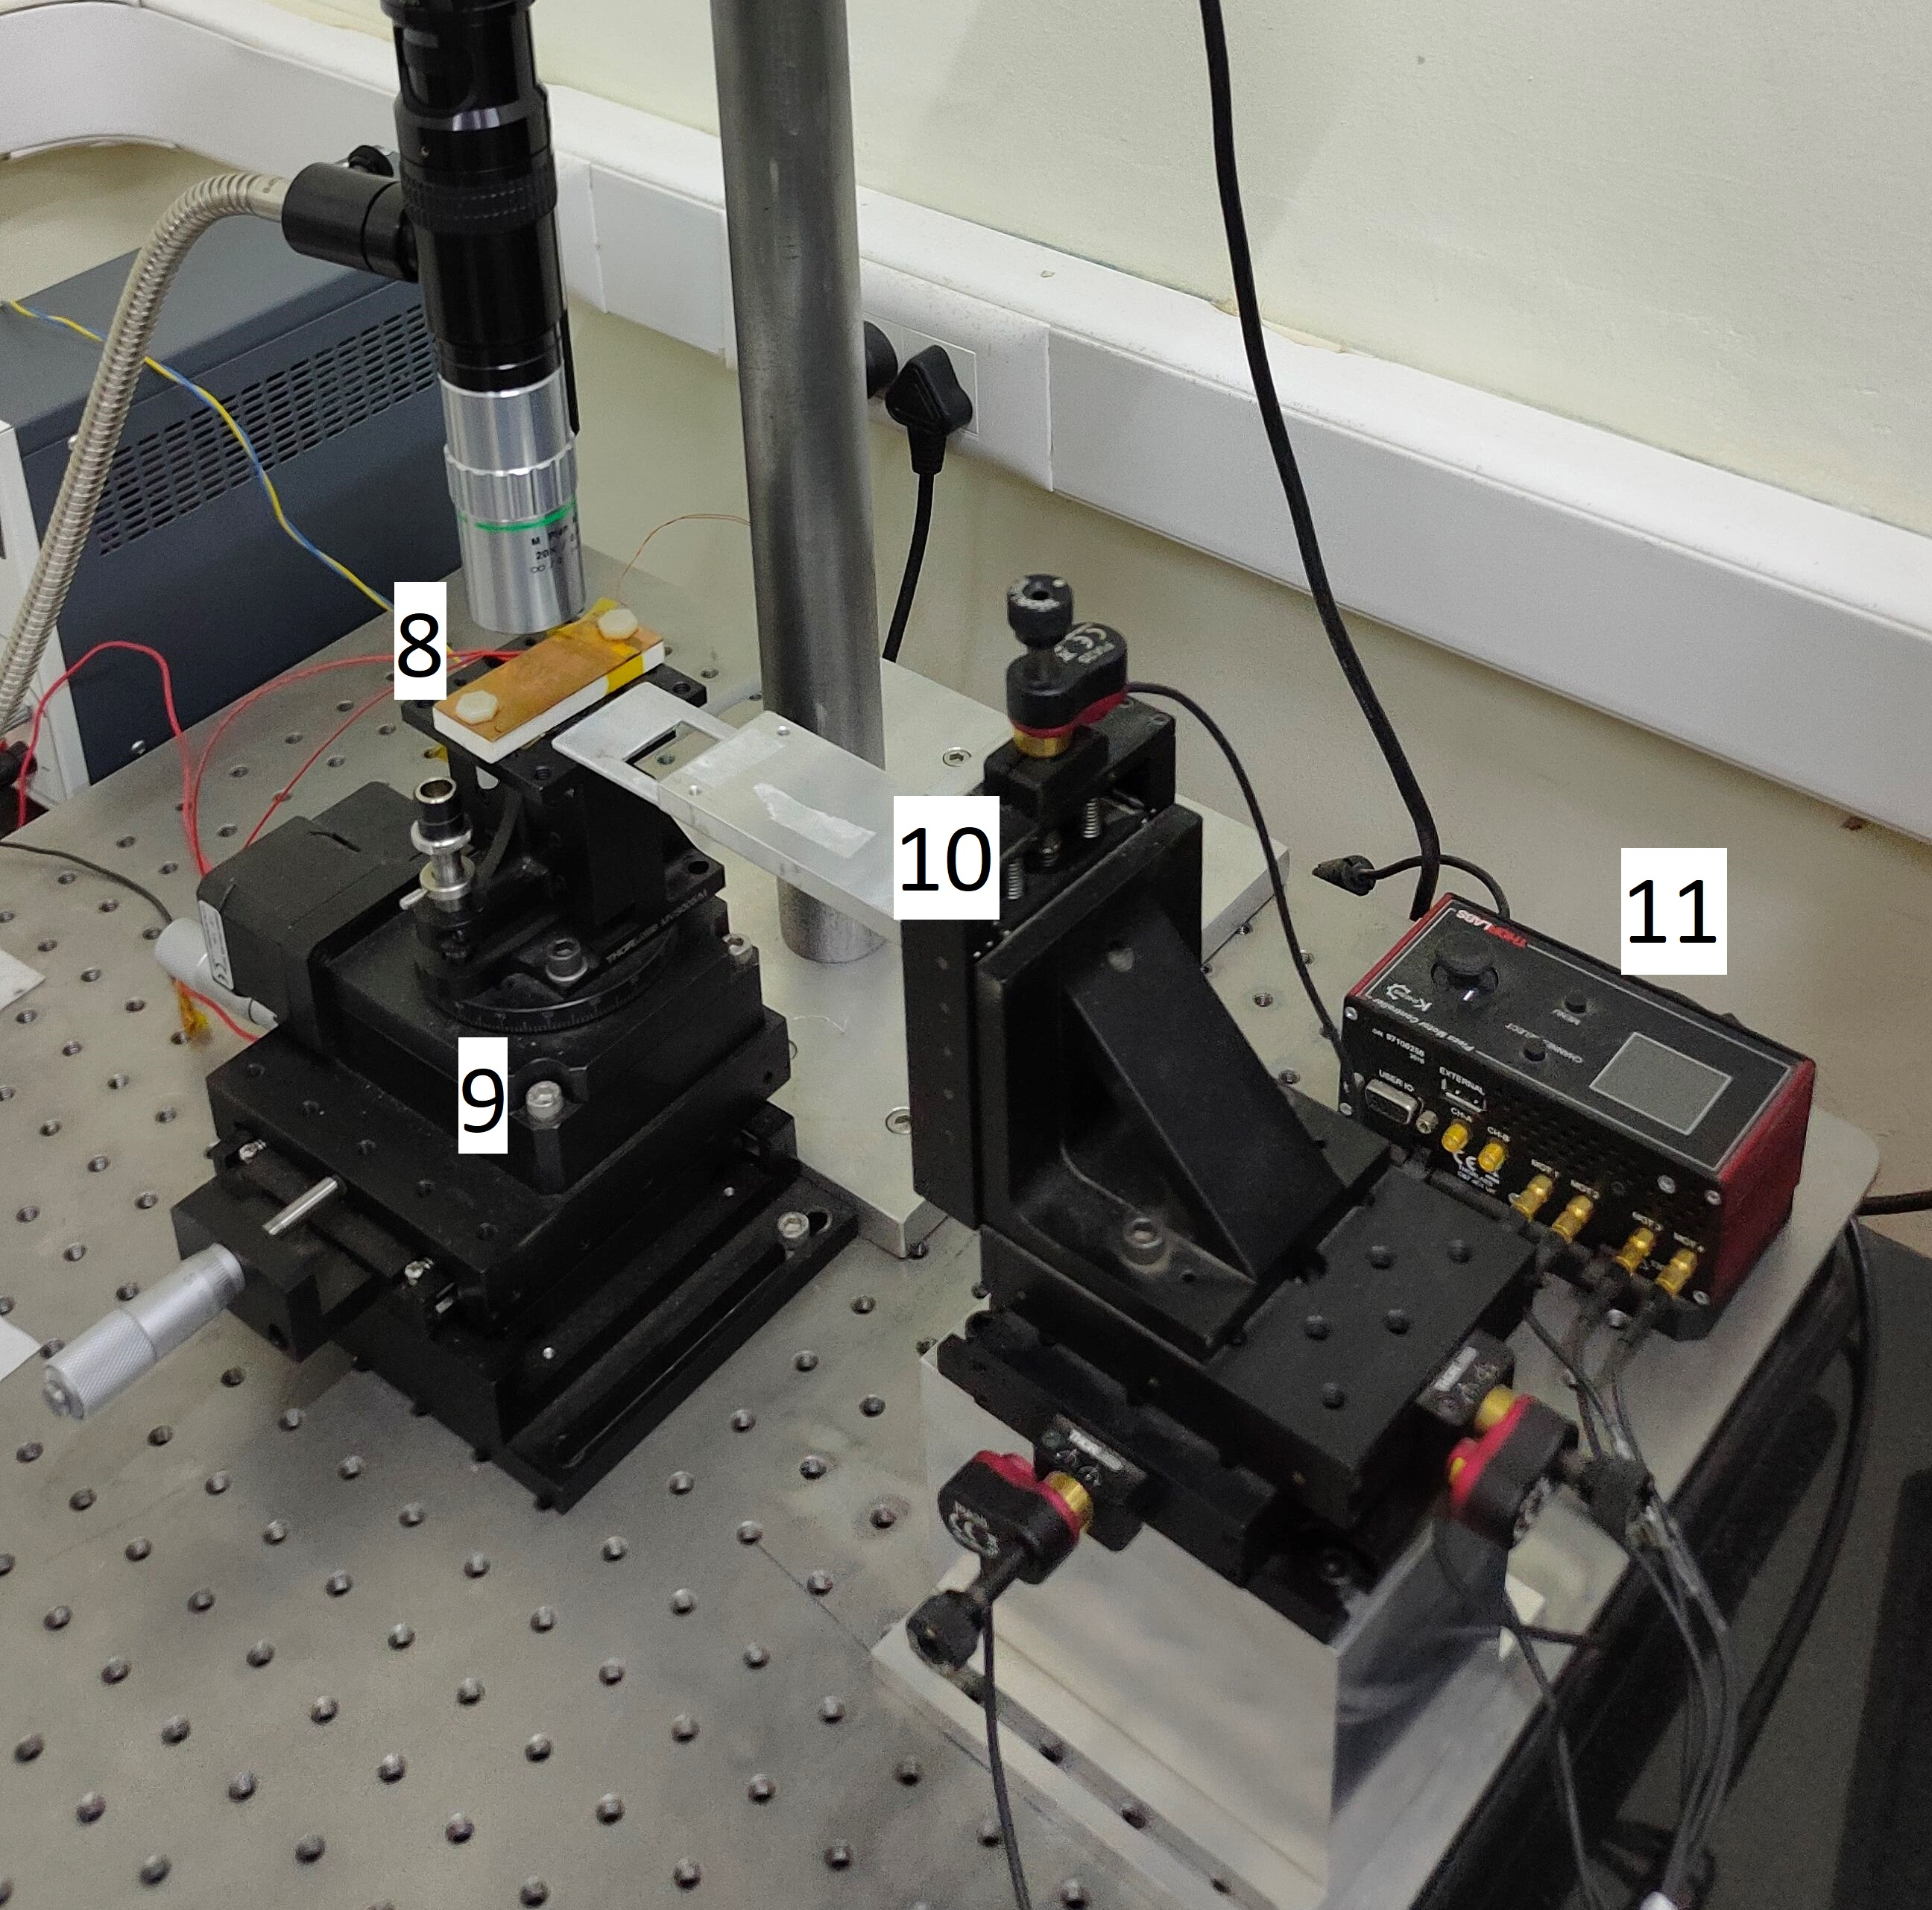
\includegraphics[width=\textwidth]{figures/trset3.jpg}
		\end{subfigure}
	\end{minipage}%
	\begin{subfigure}{0.45\textwidth}
		\centering
		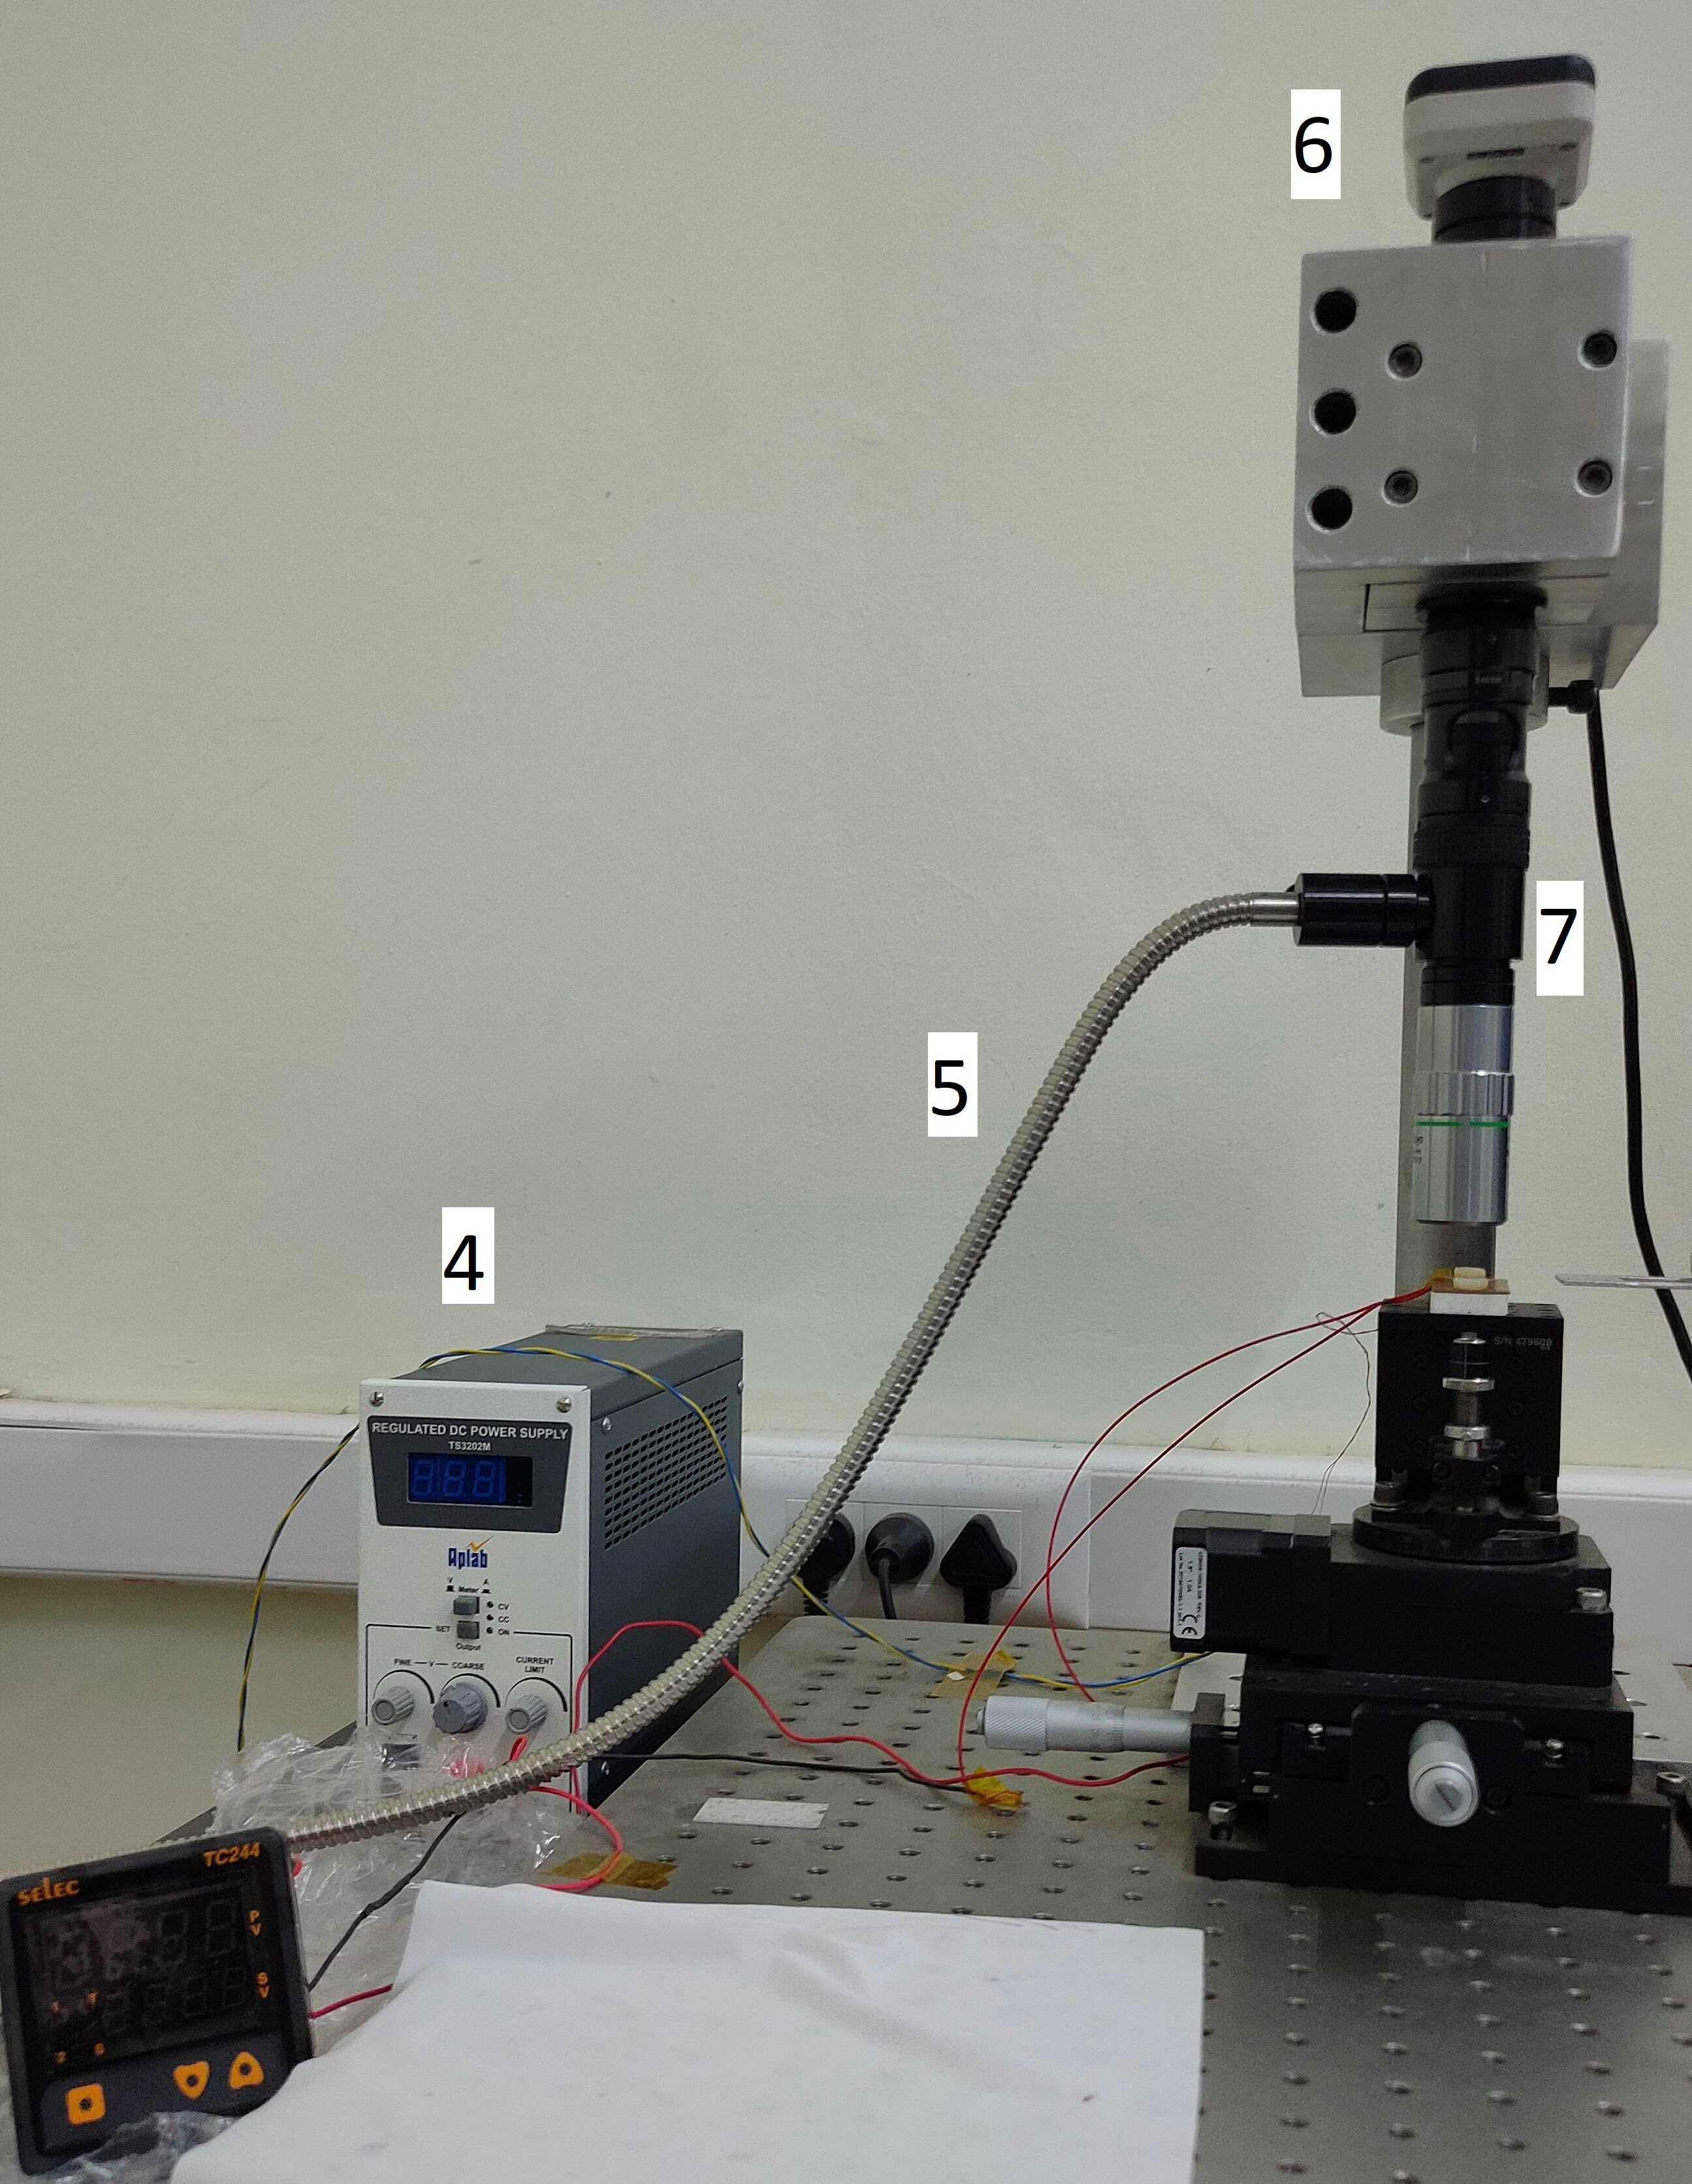
\includegraphics[width=\textwidth]{figures/trset2.jpg}
	\end{subfigure}
	\caption{Transfer Setup at lab.}
	\label{fig:tr_set}
\end{figure}

The pickup and transfer protocol is as follows:

\textbf{Part 1: Making a transfer boundary}
\begin{enumerate}
	\item Cover the microscope stage with Kapton tape and put a little square of double-sided tape on top of it.
	\item Now, a transfer boundary is made on PDMS. A piece of clean silicon wafer is stuck on the double-sided tape, and the transfer stage aluminium plate is moved between the microscope stage and the objective.
	\item Using the Piezo, the coverslip is moved vertically till the PPC-PDMS or PC-PDMS is in focus and center the region with PDMS. 
	\item The PDMS is moved up and the empty wafer is brought into focus, and the stage heater temperature is set to $63 ^o C$ for PPC ($130 ^o C$ for PC).
	\item The transfer stage is moved down slowly using the Piezo motors while keeping the wafer in focus. When the PDMS touches the wafer, a circle forms on the coverslip. The coverslip is held there for 5 seconds and then moved up.  A circular boundary will be seen on the PDMS after this step. This is the transfer boundary where the PDMS will pick up flakes.
	\item Finally, remove the wafer and the Kapton tape.
\end{enumerate}
Part 1 can be skipped once we are comfortable with the whole process.

\textbf{Part 2: Pickup Step}

\begin{enumerate}
	\item Mount the wafer with the hBN/graphene flake to be picked in the same way as before, on the double-sided tape.
	\item Follow similar steps as before, except now centre the flake to be picked, directly under the transfer circle of PDMS.
	\item Once PDMS touches the wafer, go down till the circle spreads over the flake that needs to be picked.
	\item Wait for 10 mins and turn off the heating.
	\item Wait till the temperature comes down to around $35 ^o C$. Next, move the PDMS up and confirm if the flake got picked.
	\item Finally, remove the wafer and the Kapton tape.
\end{enumerate}

\textbf{Part 3: Transfer Step}

Now there are two things that can be done. Either we keep on picking up flakes or transfer the flake/stack onto a clean wafer/gold pad. For the first case, we continue with the steps as above. We will have to take care of alignment during these steps. For the transfer, we perform the following steps:
\begin{enumerate}
	\item Cover the microscope stage with Kapton tape and put a little square of double-sided tape on top of it.
	\item Mount the wafer onto which the flake has to be transferred on the double-sided tape and heat the stage to $75 ^o C$ for PPC ($180 ^oC$ for PC)
	\item Touch the PDMS with the flake over the area to be transferred on and wait for 10 min.
	\item Move the PDMS up and check if the flake got transferred.
	\item Remove the wafer and the Kapton tape.
	\item Remove the coverslip from the aluminium plate by dissolving EL-9 using acetone.
	\item Finally, clean the coverslip and the wafer. They are kept in anisole overnight (Chloroform for 2 hours) to dissolve the PPC (PC). Wash them with IPA (IPA and acetone), and blowdry with $N_2$.
\end{enumerate}

Fig. \ref{fig:hbnongoldpad} shows the pickup of thin hBN and transfer onto the gold pad, which is a part of twisted bilayer graphene stack making. (See section \ref{section:g})

\begin{figure}[H]
	\centering
	\begin{subfigure}[b]{0.4\textwidth}
		\centering
		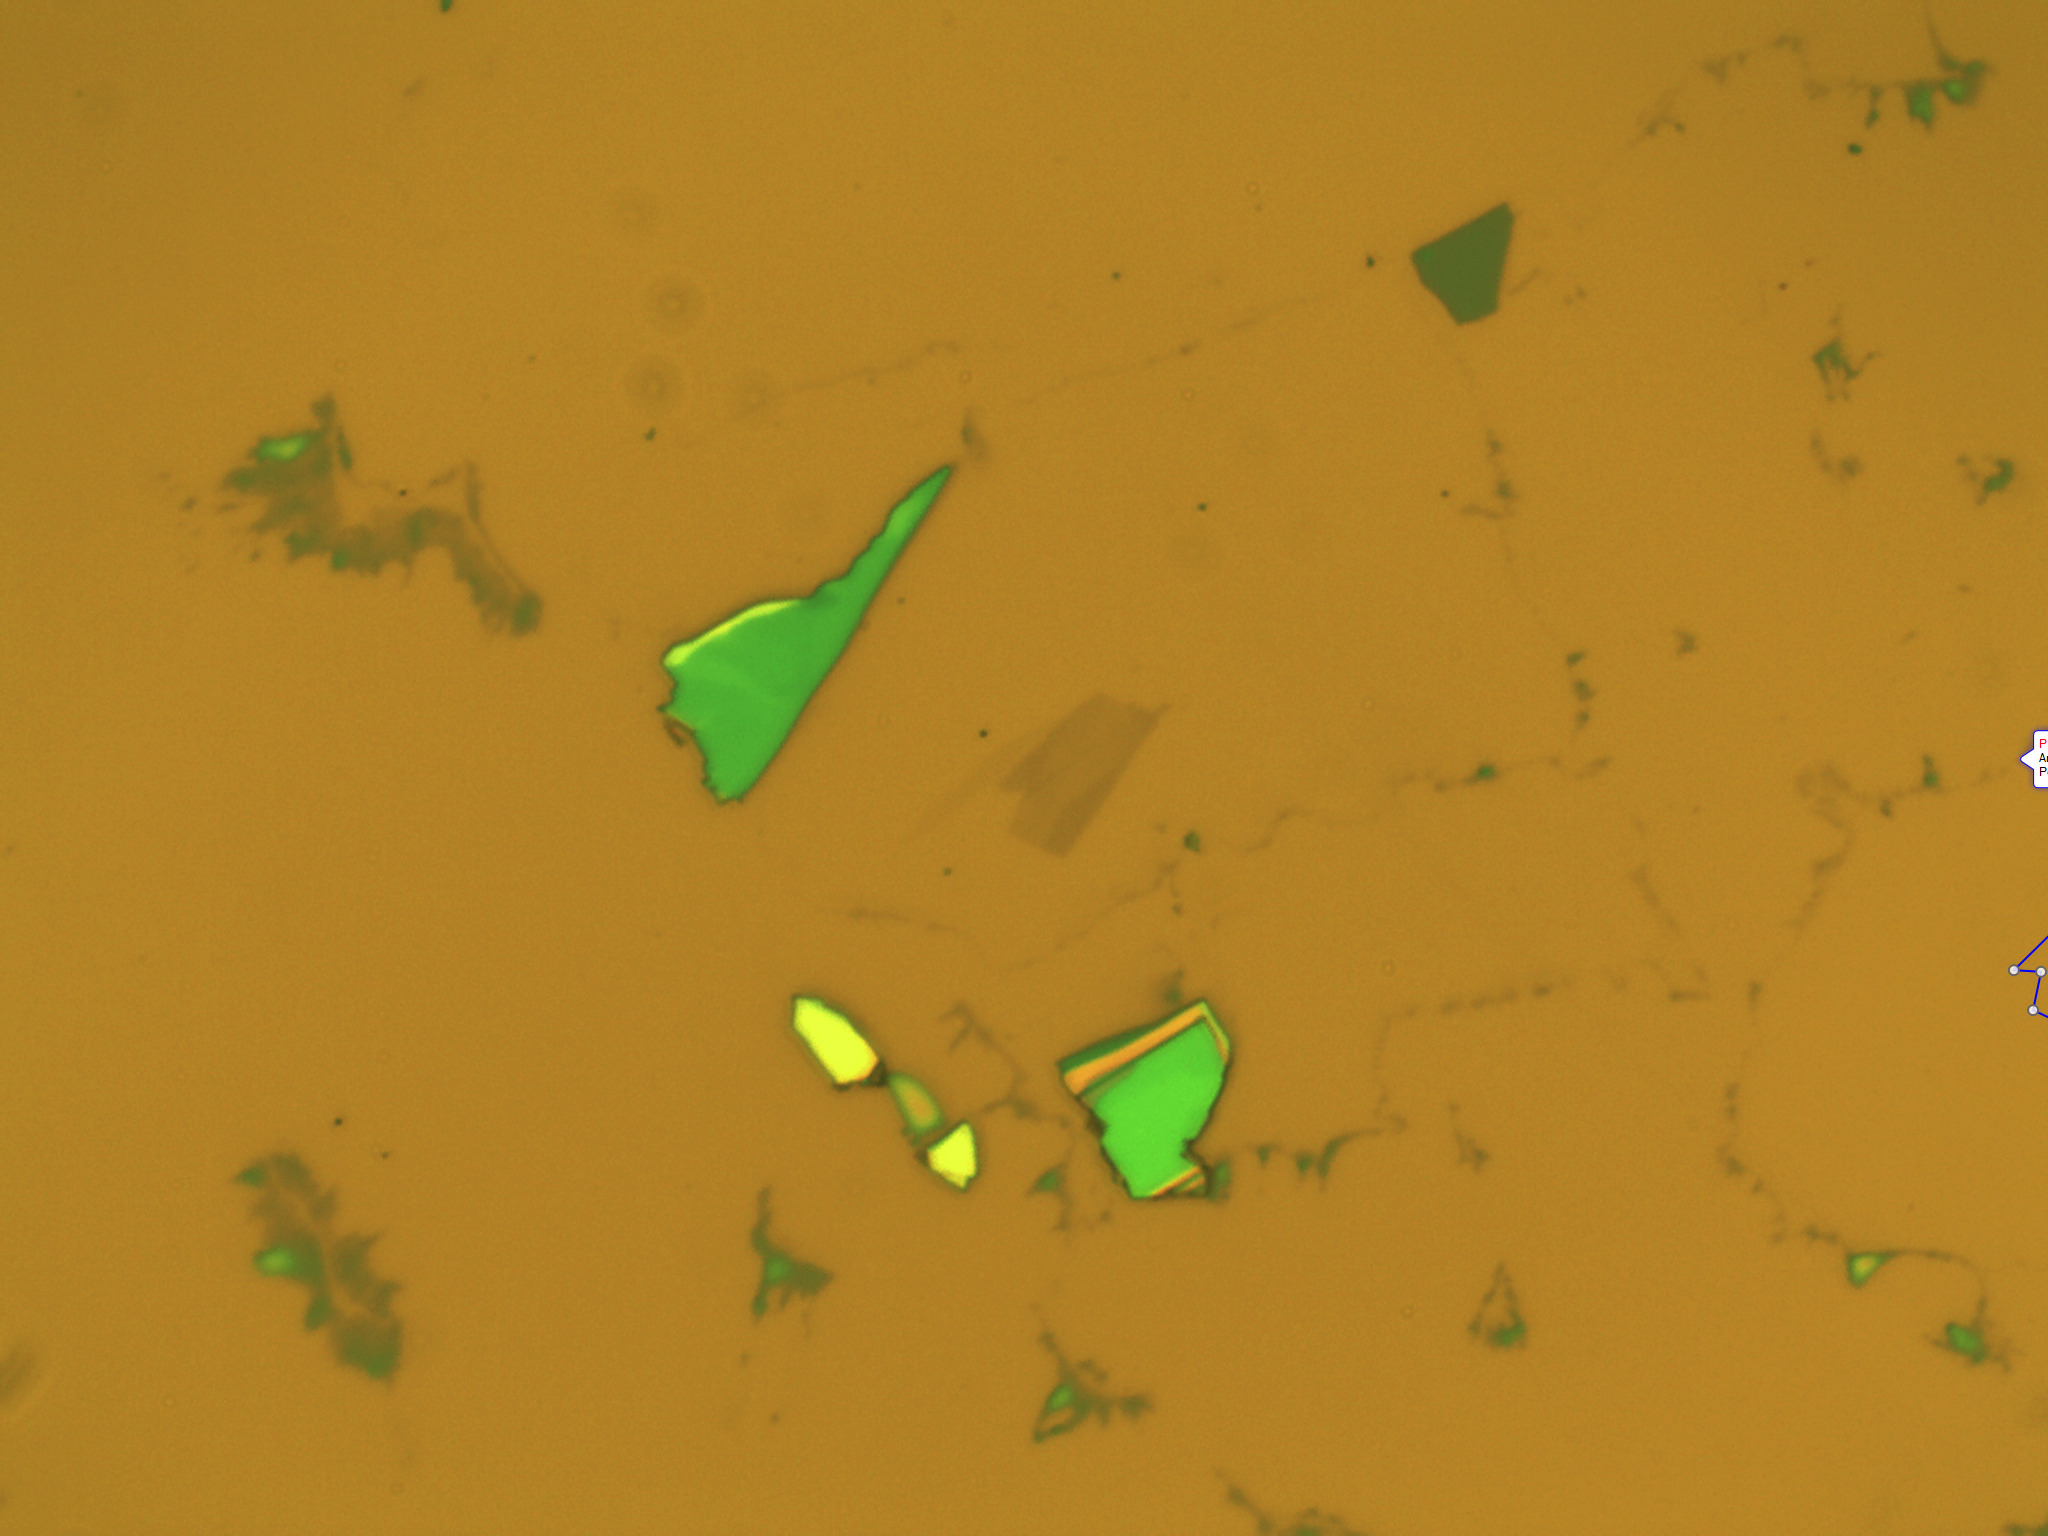
\includegraphics[width=\textwidth]{figures/hbn_before_pickup.jpg}
		\caption{tunnel hBN before pickup}
	\end{subfigure}
	\qquad
	\begin{subfigure}[b]{0.4\textwidth}
		\centering
		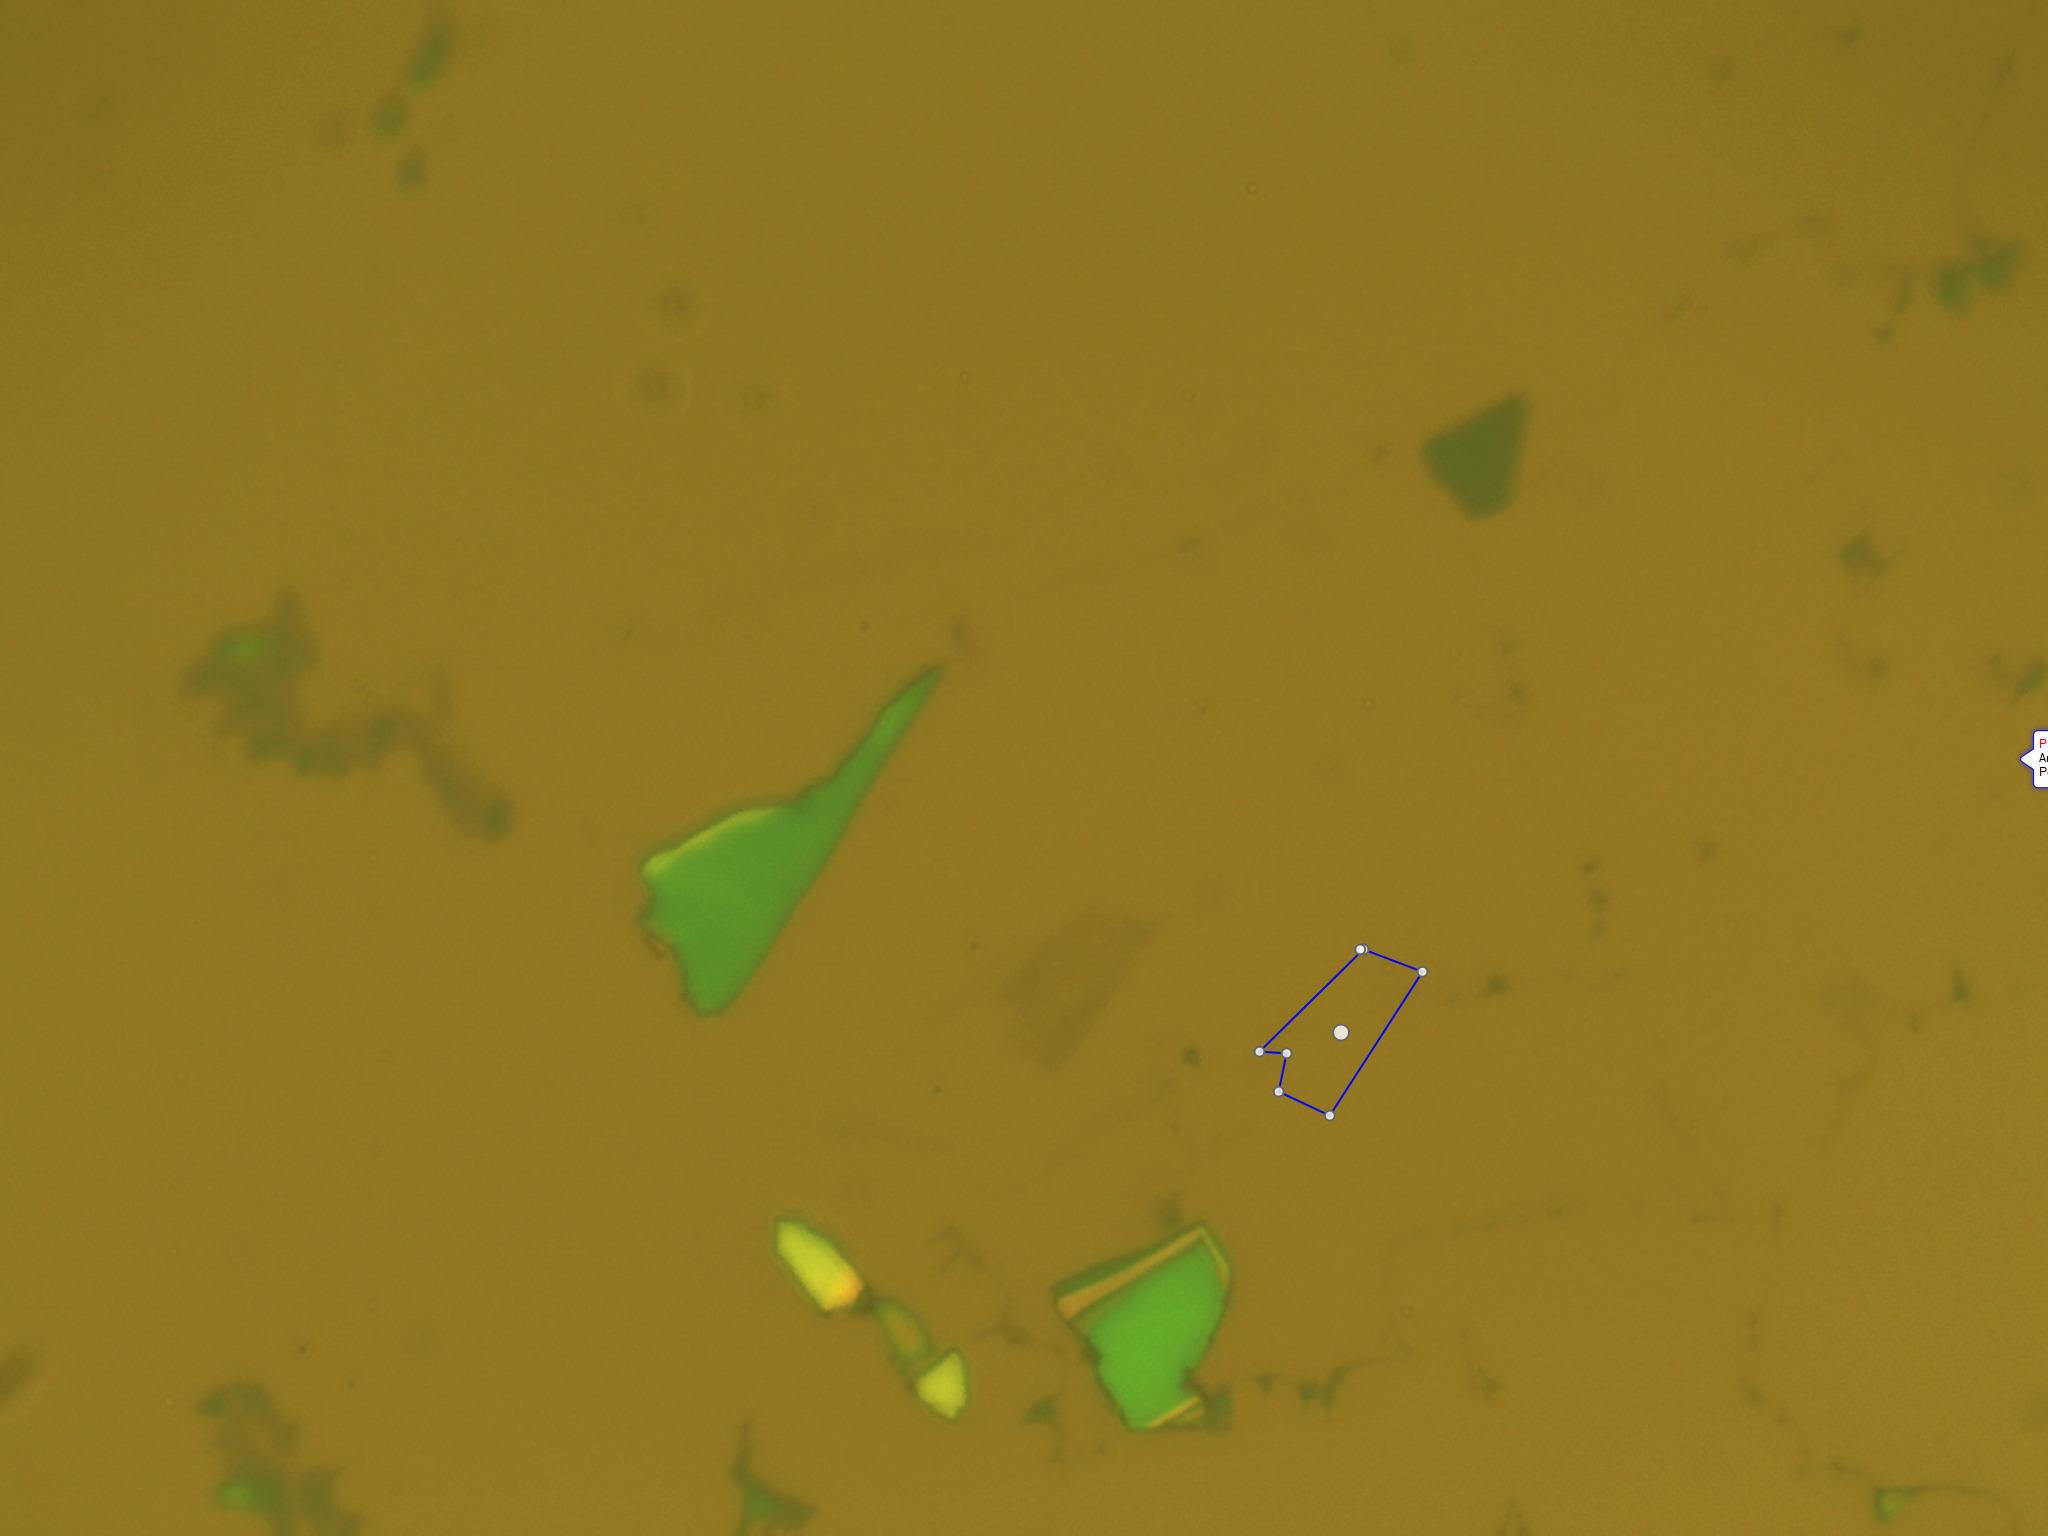
\includegraphics[width=\textwidth]{figures/hbn_through_pc.jpg}
		\caption{hBN through PC}
	\end{subfigure}
	\begin{subfigure}[b]{0.4\textwidth}
		\centering
		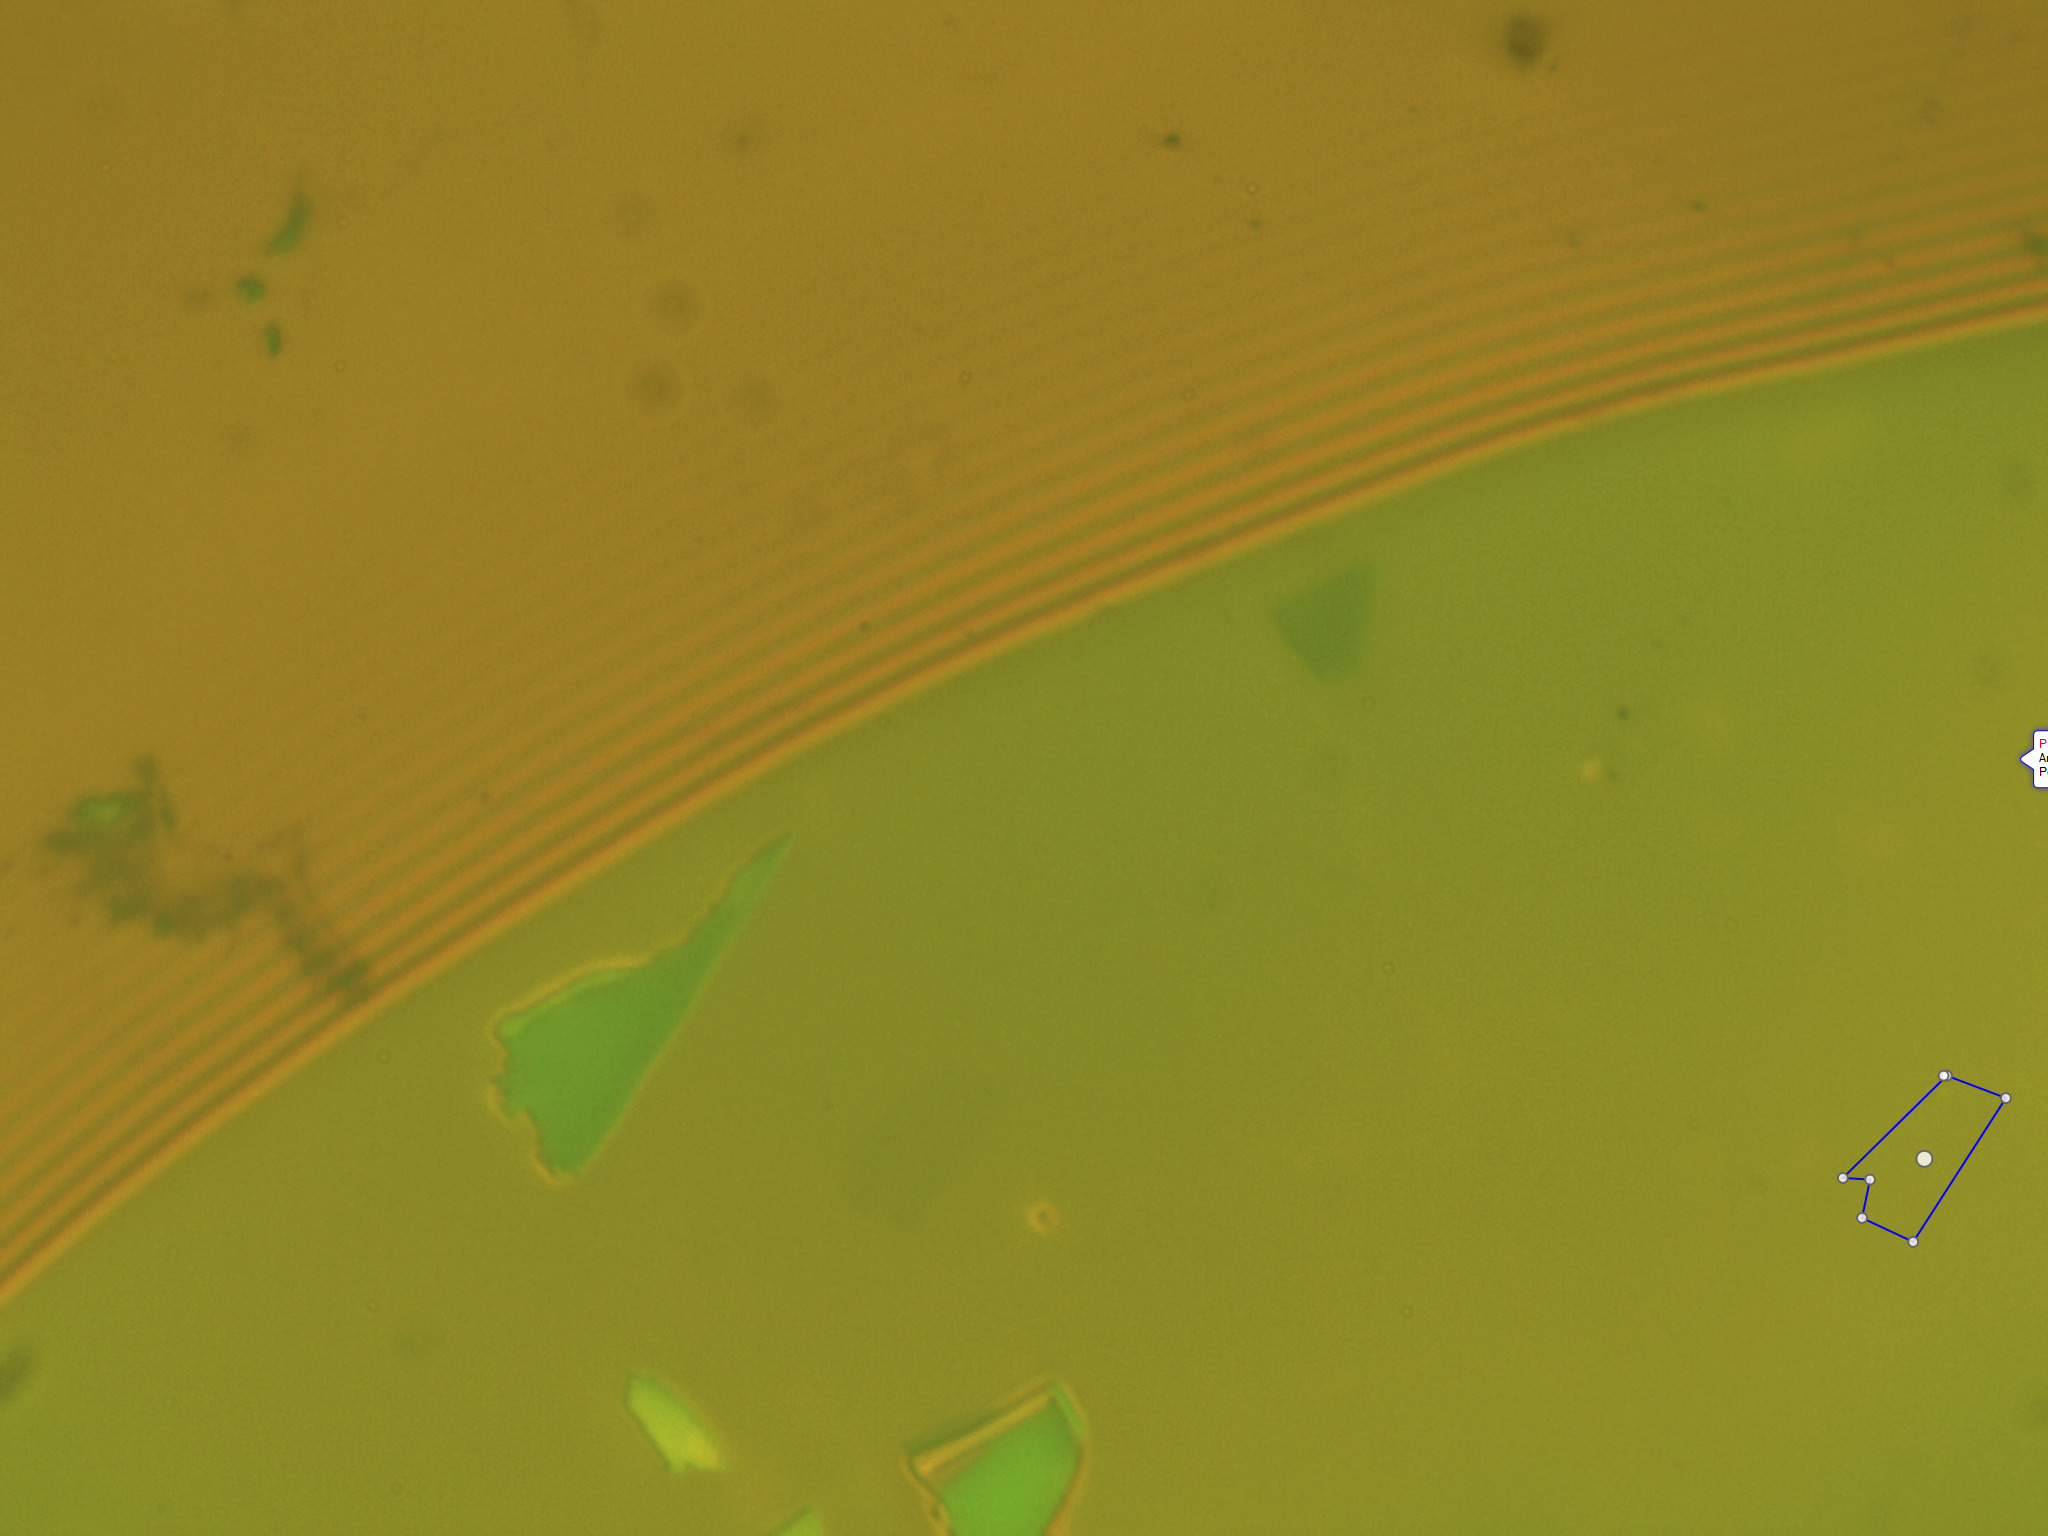
\includegraphics[width=\textwidth]{figures/during_pickup.jpg}
		\caption{During Pickup}
	\end{subfigure}
	\qquad
	\begin{subfigure}[b]{0.4\textwidth}
		\centering
		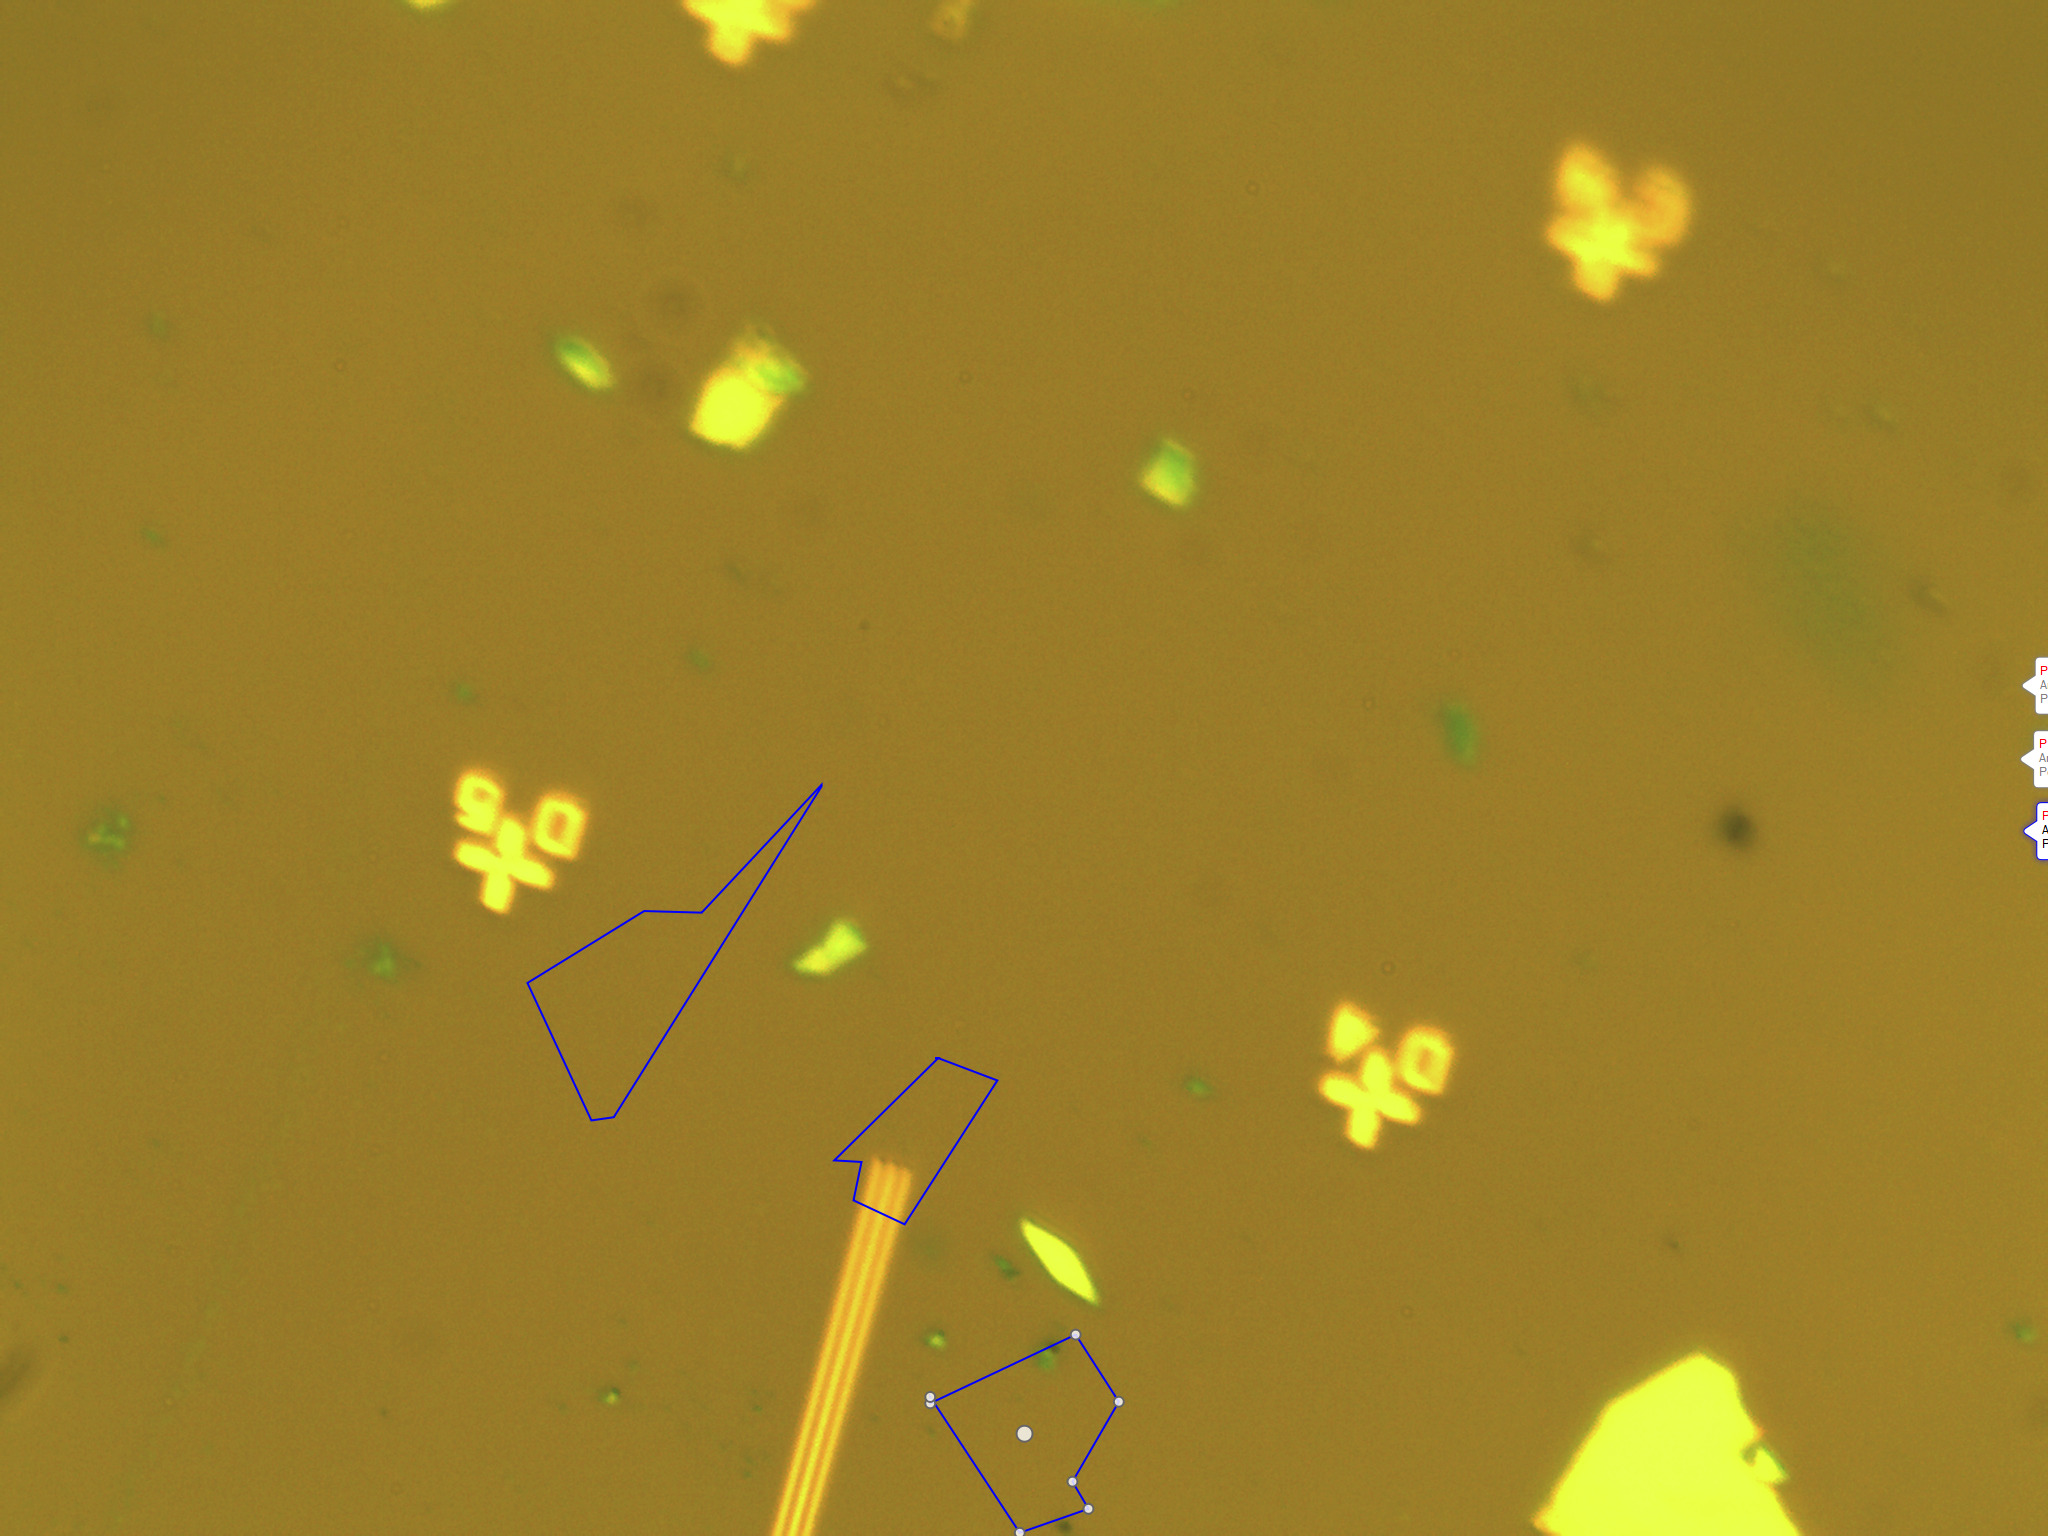
\includegraphics[width=\textwidth]{figures/gold_pad.jpg}
		\caption{Gold pad}
	\end{subfigure}
	\begin{subfigure}[b]{0.4\textwidth}
		\centering
		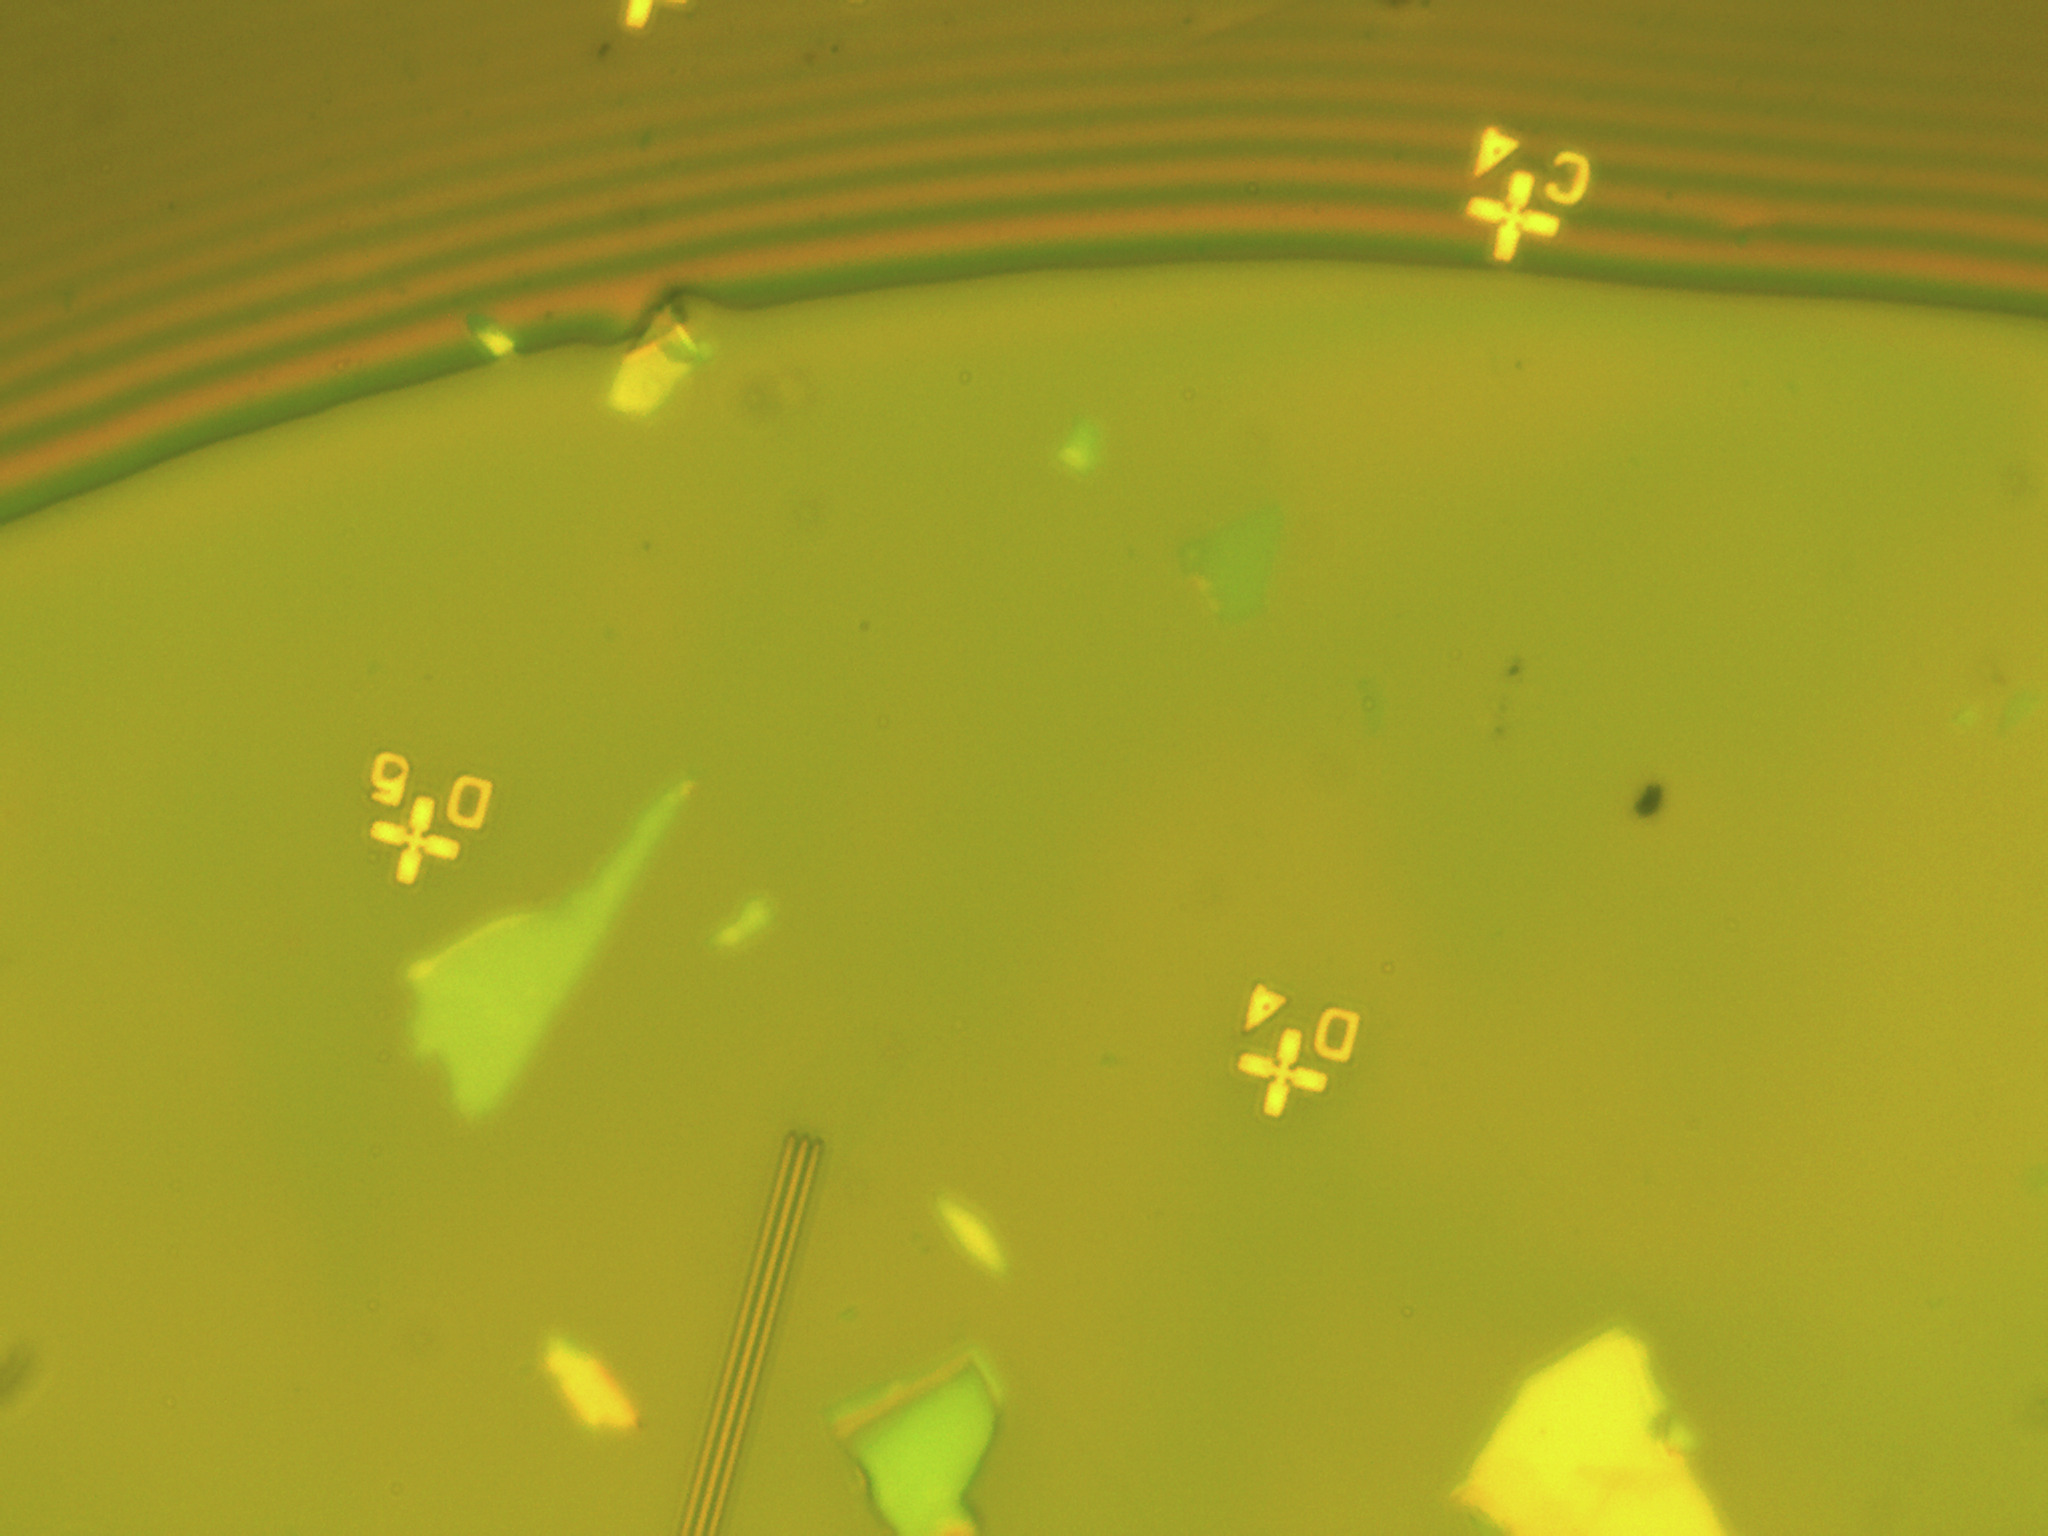
\includegraphics[width=\textwidth]{figures/during_transfer.jpg}
		\caption{During Transfer}
	\end{subfigure}
	\qquad
	\begin{subfigure}[b]{0.4\textwidth}
		\centering
		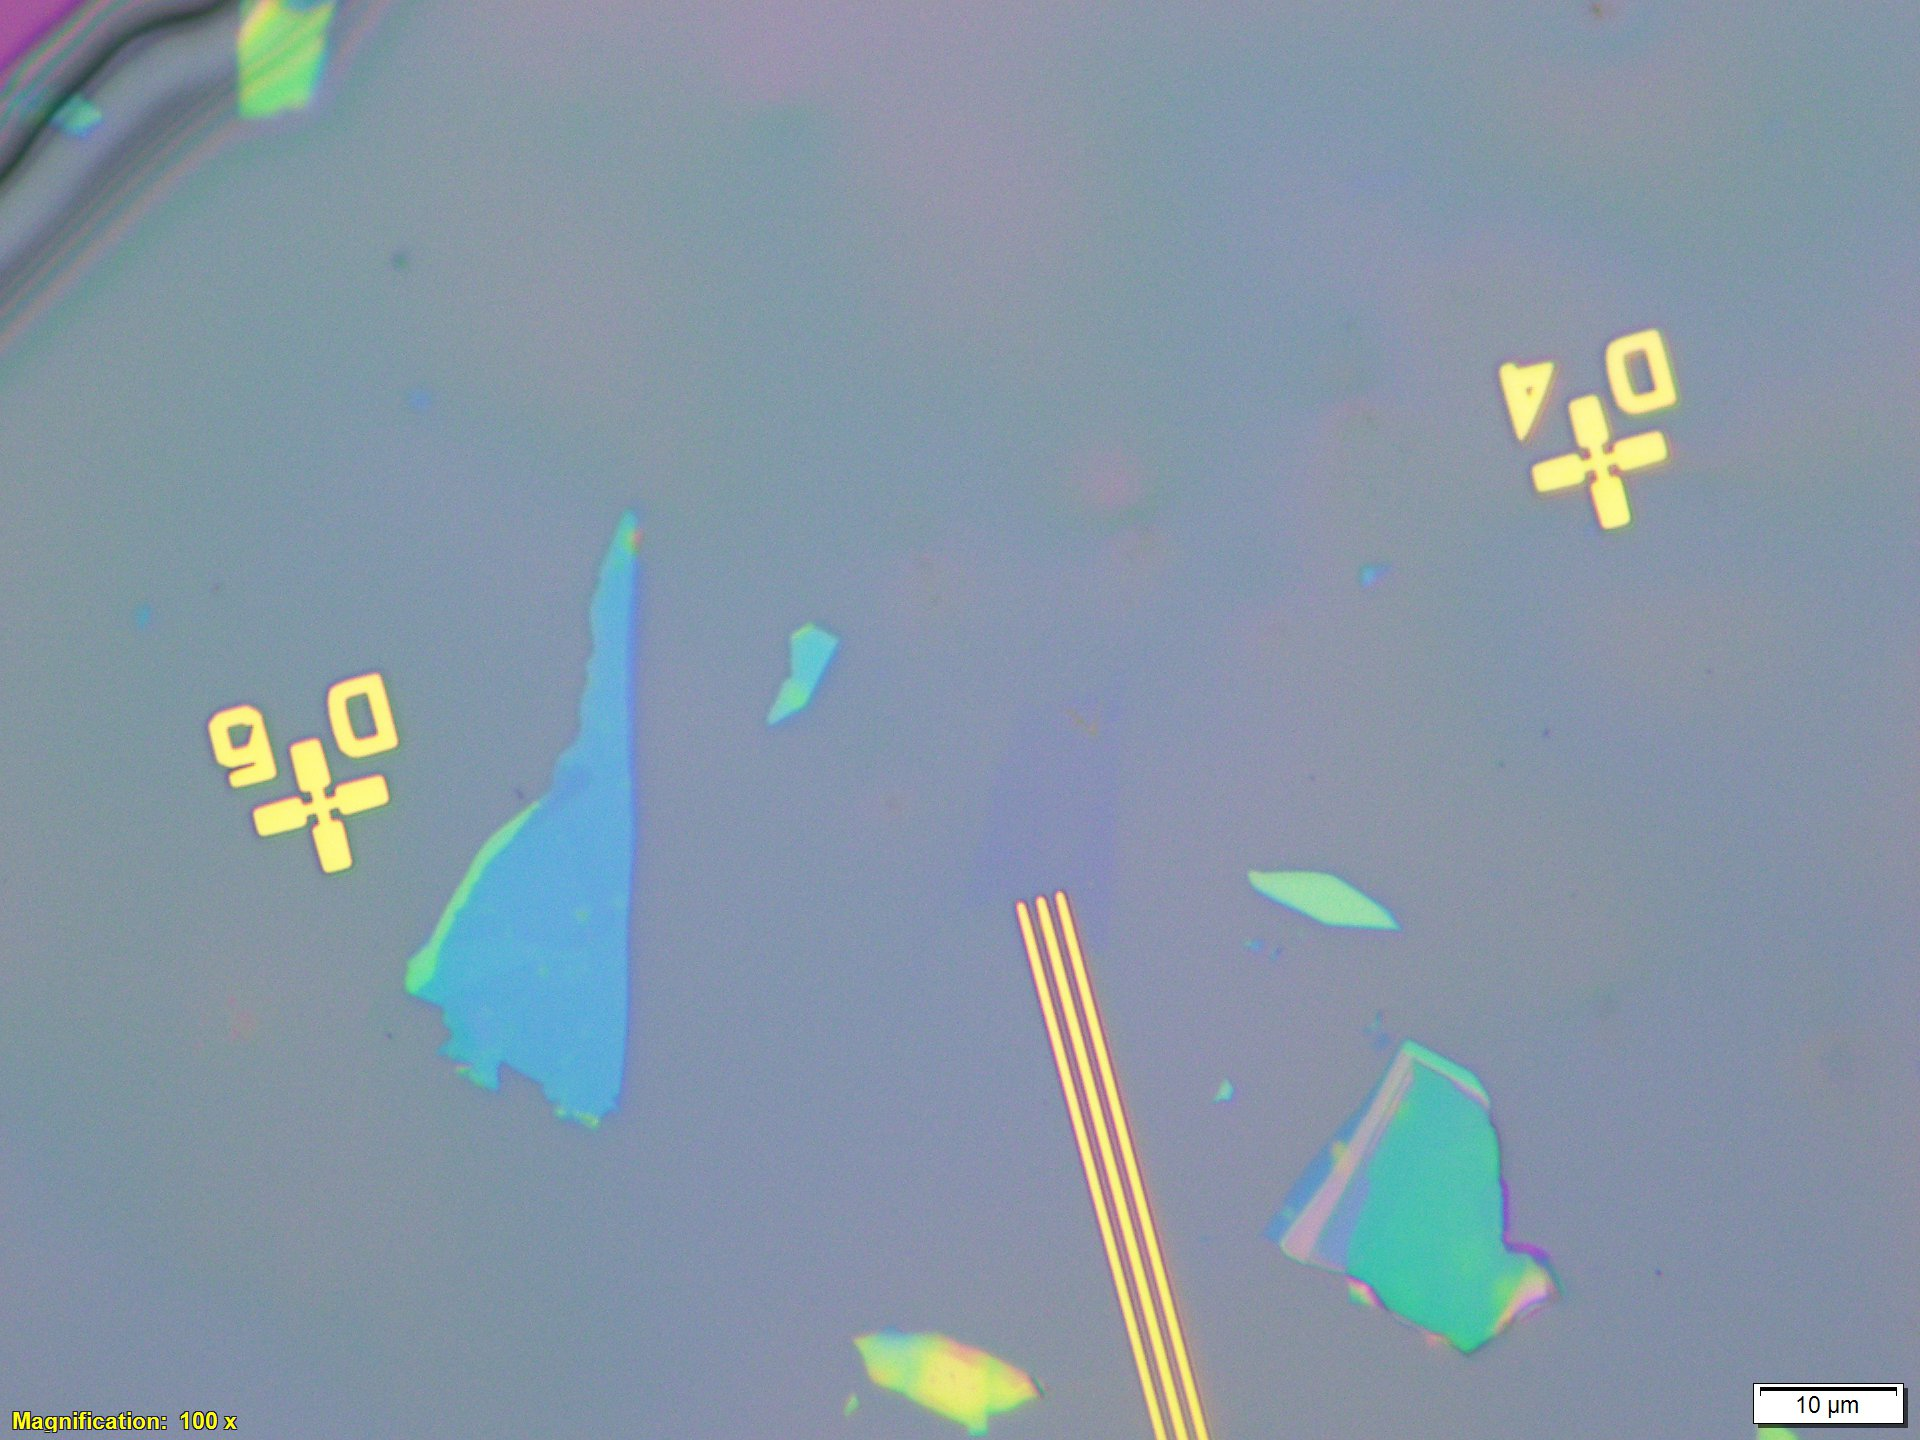
\includegraphics[width=\textwidth]{figures/after_transfer.jpg}
		\caption{After Transfer}
	\end{subfigure}
	\caption{Pickup and Transfer of thin hBN on gold pad (bottom tunneling electrode).}
	\label{fig:hbnongoldpad}
\end{figure}

\section{Twisted bilayer graphene stack}
\label{section:g}
hBN-graphene-graphene-hBN-gold pad stacks are required to be made for our devices. Here the top hBN encapsulates the twisted bilayer graphene. The two graphene flakes are aligned at magic angle of $1.1 ^o$. The hBN on the gold pad acts as a tunneling barrier. The whole process consists of two parts. One is to transfer thin hBN onto the gold pad, and the other is to make a hBN-graphene-graphene stack on PPC. We follow the protocols as mentioned in section \ref{section:f}, with one extra step during the stack preparation. The graphene is cut in half using a Pt-Ir tip (see fig. \ref{fig:tip}), and one half of the flake is picked up with hBN, the stage is twisted by $\approx1.2-1.4^o$ (the twist angle changes to $\approx 1.1^o$ due to relaxation) and the other half of the flake is picked up with graphene.

\begin{figure}[H]
	\centering
	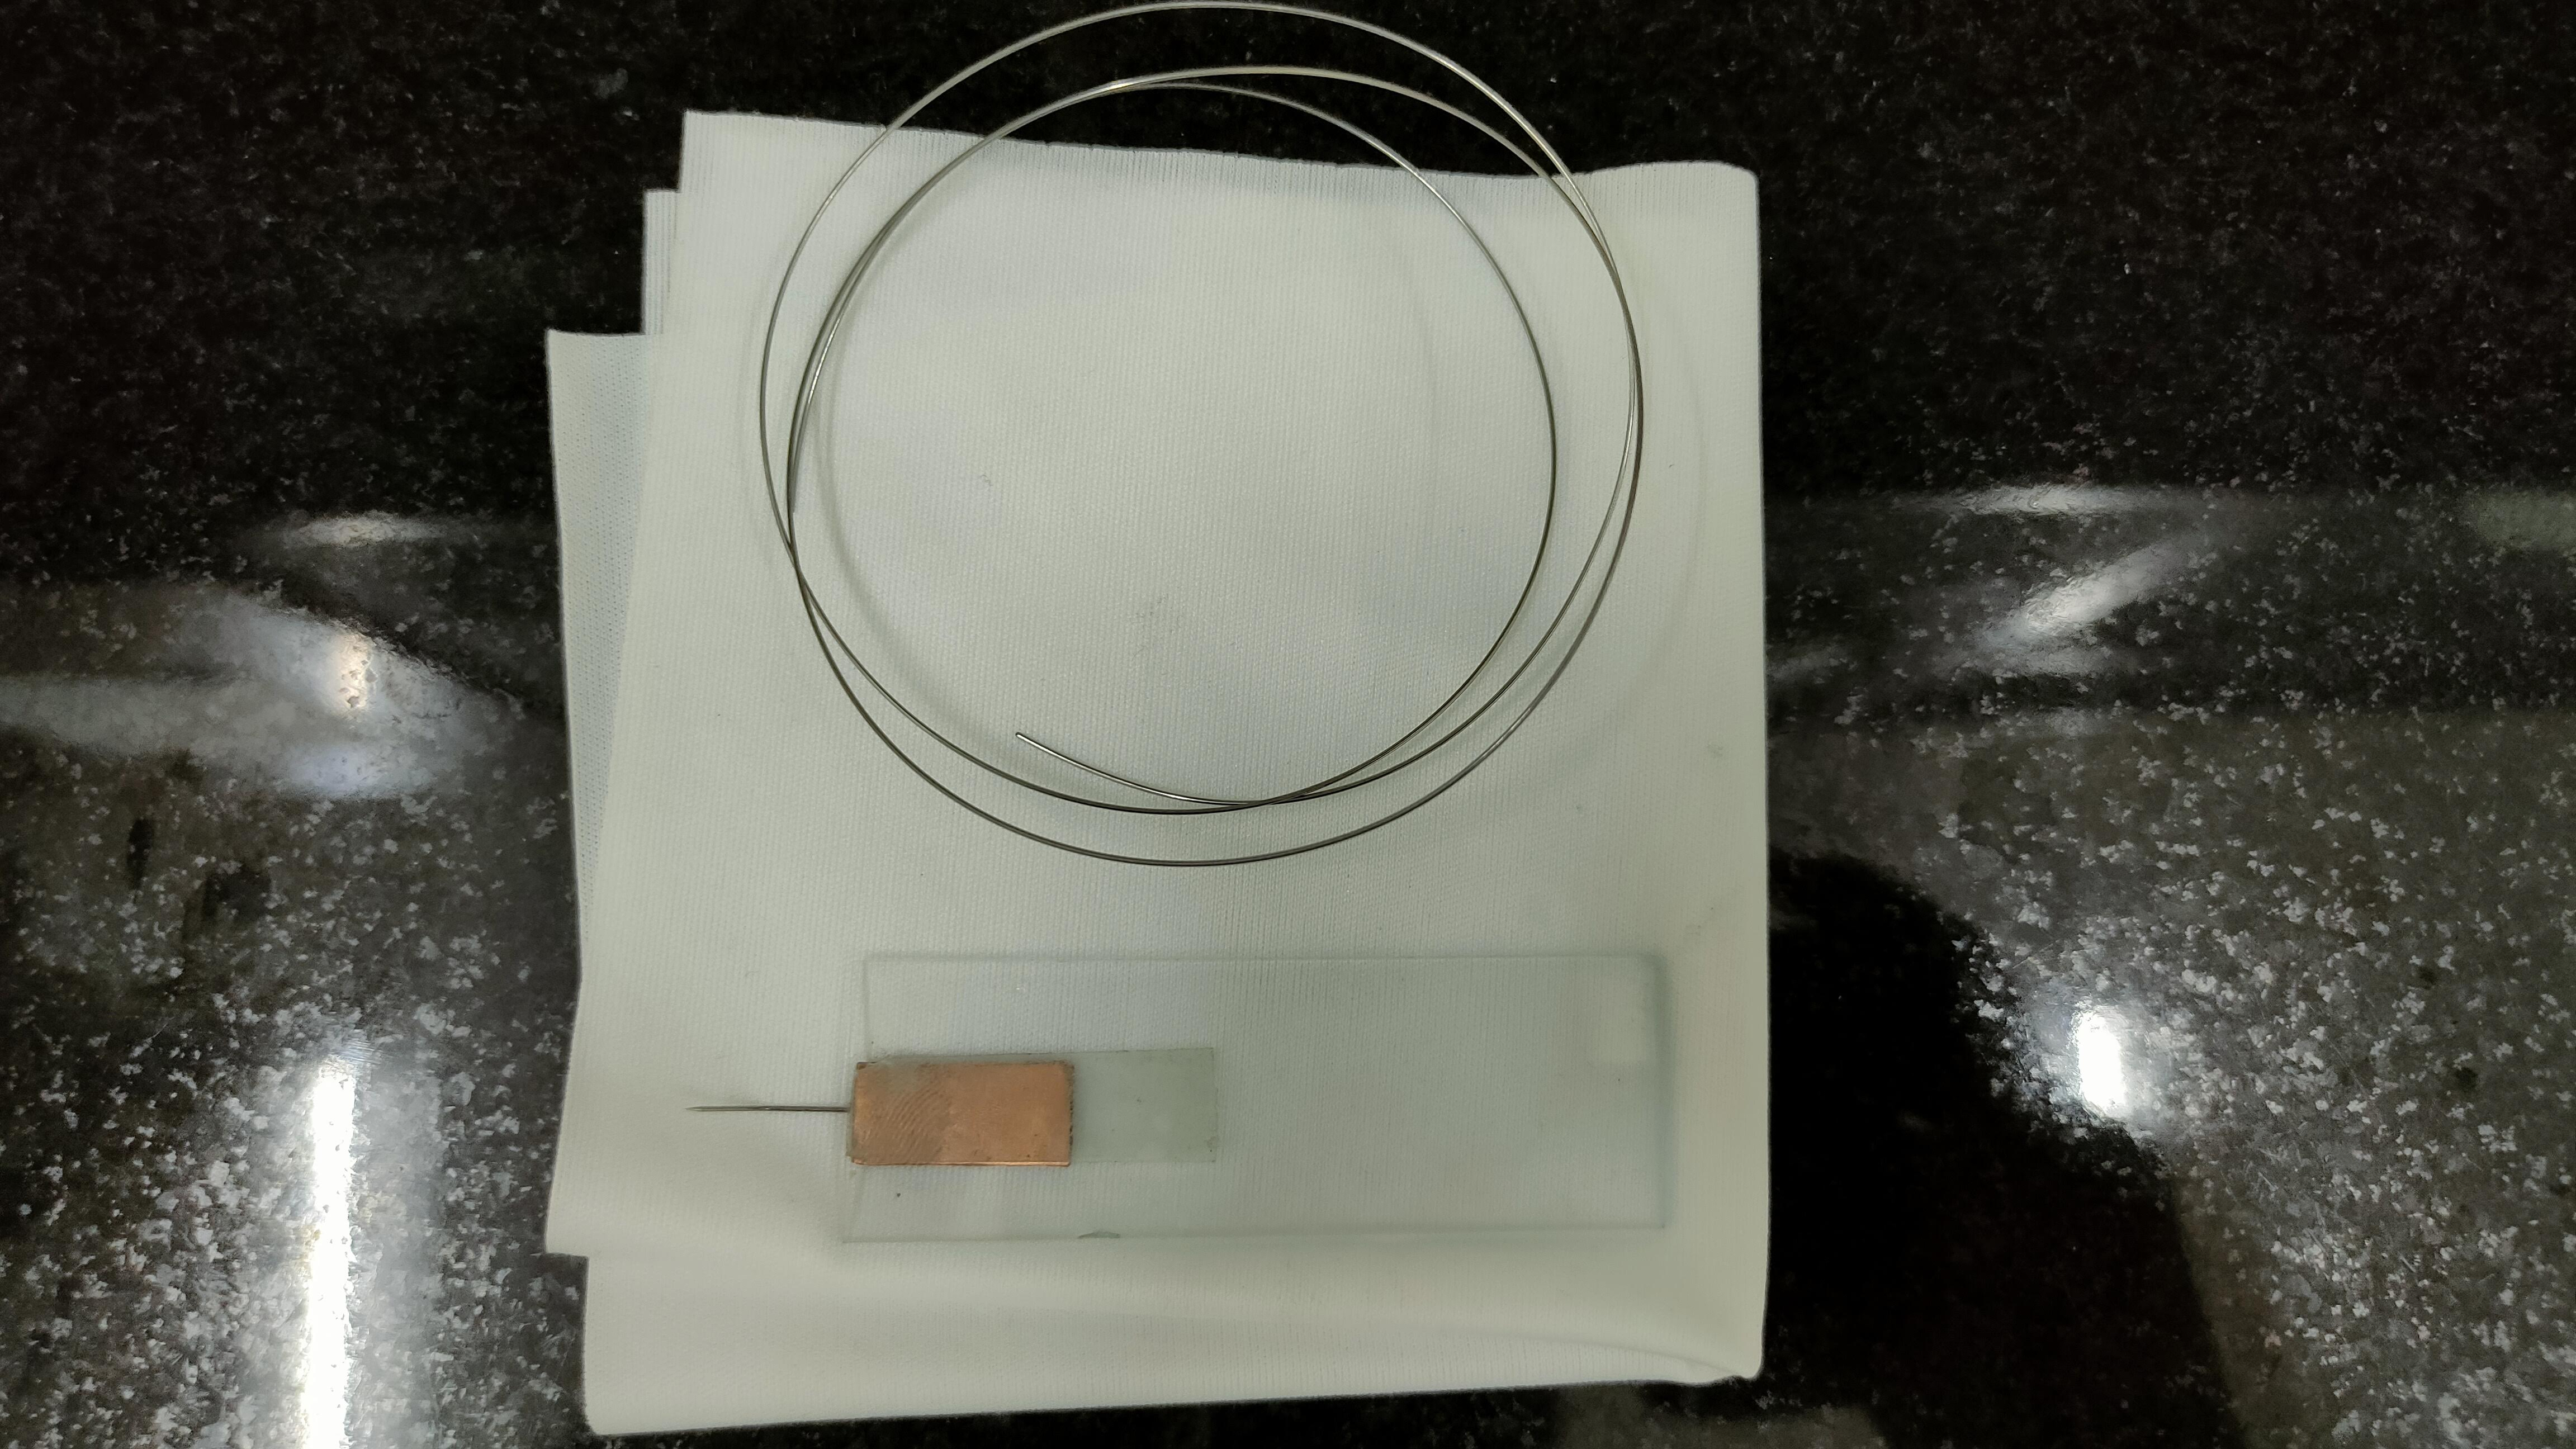
\includegraphics[width=0.7\linewidth]{figures/tip}
	\caption{Pt-Ir tip that is used in cutting graphene flake and Pt-Ir wire.}
	\label{fig:tip}
\end{figure}

The hBN-gold pad substrate is first annealed, which helps in removing residues present on the flake, making it better for using it in our device. Then the hBN-graphene-graphene stack is transferred onto the hBN-gold pad substrate, giving us the final stack. This process is called the cut and stack method. \cite{Saito2020} If the graphene is torn in half by hBN and picked up followed by picking the other half by graphene, instead of cutting the graphene with a tip, the process is called the tear and stack method. \cite{Kim16, Cao2016} Cut and stack method is preferred over tear and stack in our experiment. This is because in tear and stack, since the graphene flake is torn by hBN, it creates wrinkles and strain in the other half of the flake that is left. This will lead to an uneven angle when twisted bilayer is made, giving a bad sample.

Fig. \ref{fig:hbngrgr} shows the making of the hBN-graphene-graphene stack, which is a part of twisted bilayer graphene stack making. After stack making, there are several steps before we have sample ready for measurement: e-beam lithography, dry etching and gold deposition, which were done by Radhika.

\begin{figure}[H]
	\centering
	\begin{subfigure}[b]{0.6\textwidth}
		\centering
		\includegraphics[width=\textwidth]{figures/tophbn1.jpg}
		\caption{hBN flake before pickup that acts as top hBN}
	\end{subfigure}
	\begin{subfigure}[b]{0.6\textwidth}
		\centering
		\includegraphics[width=\textwidth]{figures/hbngr1.jpg}
		\caption{hBN flake picking up one half of the graphene flake that has already been cut}
	\end{subfigure}
	\begin{subfigure}[b]{0.6\textwidth}
		\centering
		\includegraphics[width=\textwidth]{figures/hbngrgr1.jpg}
		\caption{hBN-graphene picking up the other half of the graphene flake}
	\end{subfigure}
	\caption{Making hBN-graphene-graphene stack on PPC.}
	\label{fig:hbngrgr}
\end{figure}
